%Hierarchy is Chapter > Section > Subsection
%http://www.khirevich.com/latex/ - Tips on Writing a Thesis in LaTeX
%This is what to put in the box for bibtex: "/usr/local/texlive/2014/bin/x86_64-darwin/bibtex" %.aux
%Sometimes I might need to run bibtex on its own before doing the full quick build sequence  



\documentclass[a4paper, 11pt, oneside]{report}



%%% microtype package, for improved typesetting
\usepackage[activate={true,nocompatibility},final,tracking=true,kerning=true,spacing=true,factor=1100,stretch=10,shrink=10]{microtype}
\microtypecontext{spacing=nonfrench}
% activate={true,nocompatibility} - activate protrusion and expansion
% final - enable microtype; use "draft" to disable
% tracking=true, kerning=true, spacing=true - activate these techniques
% factor=1100 - add 10% to the protrusion amount (default is 1000)
% stretch=10, shrink=10 - reduce stretchability/shrinkability (default is 20/20)

%%% other formatting improvement or adjustment packages
\usepackage[margin=1.00in]{geometry} % set the size of all margins in inches. nominal 1.00in
\setlength{\parindent}{0em} % don't indent paragraphs
\setlength{\parskip}{1em} % space between paragraphs

%%% packages that MAY be useful for formatting but are unused unless deemed neccessary
%\usepackage{flushend} % for equalising final page column lengths. messes stuff up sometimes
%\usepackage{setspace}
%\usepackage{pdfpages}
%\hoffset = 9pt
%\voffset = 34pt

%%% font and character packages
\usepackage[T1]{fontenc} % allows for the encoding of unusual or accented characters
\usepackage[bitstream-charter]{mathdesign} % font package similar to the Elsevier font, with included maths style
\usepackage{physics} % provides a family of vector notation

%%% citation packages
\usepackage[nottoc]{tocbibind} % puts the references section into the table of contents

\usepackage{cite} % an alternative to biblatex, it still calls bibtex but unlike bibtex the citation style is defined in the line at the end of the document
\usepackage{url}

%%% packages that provide or position specific elements
\usepackage{datetime} % allows a customised was of writing the date
\usepackage{multirow} % for splitting rows inside tables
\usepackage{float} % for positioning the nomenclature floating tables
\usepackage{subcaption} % allows for captions for sub-figures

%%% packages for handling various graphics files - it seems like three of these may be doing the same thing, and should be consolidated at the end if possible
\usepackage{color} % lets text be different colours
\usepackage{graphics} % for pdf, bitmapped graphics files
\usepackage{epsfig} % for  encapsulated postscript graphics files, a type of vector image
\usepackage{epstopdf} % allows LaTeX to include EPS files by converting each one to a PDF of the same dimensions

%%% for when David wants a double-spaced version
%\linespread{2.5}

%%% for commenting out sections
\usepackage{comment}



\newdateformat{mydate}{\monthname[\THEMONTH] \THEYEAR}
\title{Sensitivity of\\Nozzle Guide Vane Flow Capacity\\to Geometric Changes}
\author{Tom Franklyn Gammage\\St John's College}
\date{\mydate\today}



\begin{document}



\maketitle



\chapter*{Abstract}


Optimal design of gas turbines depends on the accurate prediction of mass flow rate passing through all engine stages. This quantity is limited by the high-pressure turbine nozzle guide vanes (NGVs). NGV mass flow rate prediction remains a major challenge to engine designers. The lack of accurate mass flow rate prediction is driven by many uncertainties: the effect of small and unavoidable manufacturing variations; computational and conceptual difficulties in modelling 3D flows; and uncertainty of the effects of small changes in design. 

This thesis presents a simplified approach to modelling the NGV capacity (a pseudo-dimensionless mass flow rate). 2D CFD is used to simulate several mechanisms which drive capacity change for a commercial aero engine NGV. Cases without film or convection cooling are used to investigate the effects of casting variations. These baselines also allow comparison of this study's 2D capacity predictions with the manufacturer's 3D predictions. 2D and 3D are shown to be in good agreement at low pressure ratios, but at higher ratios the 2D cases under-predict the limiting (choked) mass flow rate due to unchoked secondary flows in 3D geometry.

Simulations then investigate several necessary NGV design features: the extent of the trailing edge, which contributes to the turning of flow in the NGV; the extent of the trailing edge cutback, which ensures that film cooling holes are not blocked; and the addition of pressure side film cooling, which may be required by future designs. Each of these features affects the NGV capacity. The capacity change is recorded over a range of pressure ratios typical of the geometry and design operating conditions of the part. Changes in aerodynamic performance are also discussed, these being loss and whirl angle error.

The key finding of the study is that all capacity prediction errors ultimately result from a lack of information about the effective cross-sectional area of the flow passage at various pressure ratios and chordwise locations. The thesis presents heuristics that circumvent this problem to some extent with the available data, concluding with the prediction that future heuristics can use exponentially larger (and 3D) data sets to make highly accurate and rapid capacity predictions.



\chapter*{Thanks}


I was never much of a writer. I was never much of a scientist either, which probably isn't the wisest thing to admit in an MSc thesis. Nonetheless, over the unusual course of my degree, I've been lucky enough to know several people who've helped me to write, helped me to do science, and perhaps most crucially, helped me to stick at it.

Dr David Gillespie is an exceptional thesis supervisor because he didn't just supervise the thesis -- he supervised the student too. I brought along a few unusual needs beyond the scope of the present study, which no doubt made me frustrating to work with at times. Undeterred, David helped me keep the whole thing on track. He always understood if I needed some adjustment to the schedule, or even to pause altogether. I believe this is a serious amount of patience and a real commitment to helping someone, and I cannot thank him enough. I reckon he's also helped me become a decent scientist, but I guess we'll see about that.

Chris Parton is a musicologist at Princeton University. Besides his inspiring work on Clara Schumann, he's known for inventing the Parton Method for Literature Review. You might say it's just a spreadsheet of sources, comments, and cross-references -- I say it's invaluable for keeping track of my citations, which is very welcome when all of them are some combination of the words ``cooling'', ``turbine'', and ``vane''. Chris has been a very dear friend and partner in silly ideas for a long time, which makes him both a help-to-write person and a help-to-stick-at-it person. Double points for Chris and good luck to him in finishing his PhD. He'd better not forget to thank me.

Prof Jayne Franklyn and Prof Michael Gammage have recently returned to academia as my official proof-readers. The pay's not great but at least they get to laugh at my spelling. Mum, you were right about my referencing style. And about all your other comments too. Love you both.

Alison Woodward is an absurdly talented economist who's about to move home to Canberra with me, where we'll have a front garden in which we grow kaffir lime trees and old Fords. As a member of the workforce, she's how I've been able to finish my degree. As Alison, she's \textit{why} I've been able to finish my degree. What more is there to say? Let's go on an adventure.

TMFG \newline
\date{\mydate\today}



\tableofcontents
\listoffigures
\listoftables



\chapter*{Nomenclature}


\subsection*{Romans}
\begin{table}[H]
\begin{center}
\begin{tabular}{ll}
$p$ & Pressure \\
$Q_{23}$ & Rate of heat addition, ideal Brayton cycle \\
$\dot{m_i}$ & Mass flow rate, ideal Brayton cycle \\
$T$ & Temperature \\
$H_{LV}$ & Jet fuel lower heating value \\
$\dot{m_f}$ & Fuel mass flow rate, ideal Brayton cycle \\
$r_p$ & Engine pressure ratio, ideal Brayton cycle \\
$\dot{m}$ & Nozzle mass flow rate \\
$u$ & Velocity \\
$A$ & Nozzle throat area \\
$r$ & Nozzle pressure ratio \\
$r_c$ & Nozzle critical pressure ratio, $0.5379$ \\
$A_{eff}$ & Nozzle effective throat area \\
$\vu*{u}$ & Local velocity unit vector on sonic line \\
$\vu*{r}$ & Sonic line local unit direction vector \\
$dL$ & Infinitesimal length on sonic line \\
$L$ & Nozzle guide vane characteristic length for Reynolds number \\
$Re$ & Reynolds number \\
$M$ & Mach number \\
$y$ & Distance from wall within boundary layer \\
$y_+$ & Dimensionless distance from wall within boundary layer \\
$u_f$ & Friction velocity within boundary layer \\
$\tau_w$ & Wall shear stress \\
$C_f$ & Wall skin friction coefficient \\
$C_{pt}$ & Total pressure loss coefficient \\
$C_{Gao}$ & Total pressure loss coefficient (Gao) \\
$Y$ & Coolant/mainstream mass flow rate ratio \\
$x$ & Distance \\
$\dot{m_c}$ & Film coolant mass flow rate \\
$A_h$ & Cooling hole cross-sectional area \\
$M_{isent}$ & Nozzle guide vane surface isentropic Mach number
\end{tabular}
\end{center}
\end{table}

\subsection*{Greeks}
\begin{table}[H]
\begin{center}
\begin{tabular}{ll}
$\eta_{th}$ & Thermal efficiency, ideal Brayton cycle \\
$\eta_h$ & Heating efficiency, ideal Brayton cycle \\
$\rho$ & Density \\
$\Gamma$ & Nozzle flow capacity \\
$\sigma$ & Scale constant \\
$\Gamma_c$ & Choked nozzle flow capacity \\
$\delta$ & Approximate maximum thickness of a turbulent boundary layer \\
$\mu$ & Dynamic viscosity \\
$\zeta$ & Kinetic energy loss coefficient \\
$\lambda$ & Iterative substitute for $p_{0c}$ \\
$\zeta_c$ & Coolant loss coefficient \\
$\Gamma_{in}$ & Film cooled nozzle flow capacity at domain inlet \\
$\Gamma_{out}$ & Film cooled nozzle flow capacity at domain outlet \\
$\Gamma_c$ & Film coolant plenum flow capacity
\end{tabular}
\end{center}
\end{table}

\subsection*{Subscripts}
\begin{table}[H]
\begin{center}
\begin{tabular}{ll}
$i1$, $i2$, $i3$, $i4$ & Ideal Brayton cycle salient points \\
$0$ & Total \\
$1$ & At the domain inlet \\
$2$ & At the domain outlet \\
$uc$ & Uncooled case \\
$wake$ & Within the nozzle guide vane wake region \\
$cp$ & At the cooling plenum domain boundary \\
$c$ & At the cooling hole exit
\end{tabular}
\end{center}
\end{table}

\subsection*{Constants}
\begin{table}[H]
\begin{center}
\begin{tabular}{ll}
$\gamma$ & Ratio of specific heats for air, $\approx 1.4$ \\
$c_p$ & Specific heat of air at constant pressure, $\approx 1121$ $\frac{J}{kg K}$ \\
$R$ & Specific gas constant for air, $287.058$ $\frac{J}{kg K}$
\end{tabular}
\end{center}
\end{table}

\subsection*{Abbreviations}
\begin{table}[H]
\begin{center}
\begin{tabular}{ll}
NGV & Nozzle guide vane \\
CFD & Computational fluid dynamics \\
IC & Internal combustion \\
FMG & Full multi-grid initialisation (Fluent) \\
k-$\omega$ SST & Menter's shear stress transport turbulence model \\
2D & 2-dimensional \\
3D & 3-dimensional \\
XWB & Extra-wide body (Airbus A350 XWB with Trent XWB) \\
KE & Kinetic energy \\
PR & Pressure ratio \\
CMC & Ceramic matrix composite \\
OPR & Overall pressure ratio \\
84K & $84,000$ $lbf$ thrust \\
97K & $97,000$ $lbf$ thrust
\end{tabular}
\end{center}
\end{table}



\chapter{Introduction}
\label{chapter_introduction}
%--Include some derivation of how capacity prediction errors can cause exponentially increasing errors in later stages
%--In the relevant chapter, extend capacity to 2D to show how it becomes more nuanced

%definition is done and good. next steps to add:

%--we know that geometry and pr are the ONLY drivers of Aeff, but we don't know HOW geometry drives changes.

Jet engines cannot achieve a reversible, adiabatic cycle. Although the principle of operation is based on the ideal Brayton thermodynamic cycle, the design space for a real engine is bounded by the capabilities of the available materials, the means of manufacture, and the design of the components. The differences between the ideal cycle and the real engine operation cannot be fully understood using contemporary low-order models. Consequently it remains extremely difficult to accurately predict the engine core mass flow rate, despite this quantity being essential for optimal engine design.

A key factor in overall engine size, and thus weight, is the required geometric throat area of the high pressure turbine nozzle guide vanes (NGVs). These are the set of stationary vanes upstream of the rotor, which impart whirl to the hot high-pressure combustion products leaving the combustor. The NGV annulus sets the mass flow rate through the engine core, and thus sizes the engine, but it is not a perfect nozzle and is subject to losses. Lack of knowledge of loss mechanisms typically leads to over-prediction of the NGV capacity. When the manufactured engine operating condition is adjusted to achieve the required thrust, the aerodynamic matching of components is compromised.

This thesis analyses the high-pressure turbine NGVs. The study investigates how the pseudo-dimensionless mass flow rate, \textit{flow capacity}, is affected by various design parameters necessary to achieve a cooled, long-life NGV. Furthermore the sensitivity of flow capacity to small manufacturing tolerance errors is characterised. Further analyses examine the aerodynamic performance of this component in terms of its ability to impart the correct whirl angle to the post-combustor flow with minimal loss, so as to most efficiently deliver the flow to the high pressure turbine and beyond.



\section{Motivation}

For the engine manufacturer, the penalty for over-predicting flow capacity is an engine with a larger nacelle, as the bypass air must be ducted around a larger core. For the aircraft manufacturer, this incurs the severe penalties of increased drag and increased weight, affecting fuel consumption, range, and passenger capacity.

The requirement for an accurate core mass flow rate prediction may be illustrated by consideration of the ideal Brayton thermodynamic cycle, which is plotted in Figure~\ref{fig:brayton_cycle_plots}.

\begin{figure}[H]
	\centering
	\begin{subfigure}{.45\textwidth}
		\centering
		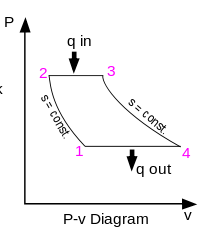
\includegraphics[width=\linewidth]{figs/brayton_cycle_pv_plot.png}
		\caption{p-v plot}
		\label{fig:brayton_cycle_pv_plot}
	\end{subfigure}
	\hspace{0.05\textwidth}
	\begin{subfigure}{.45\textwidth}
		\centering
		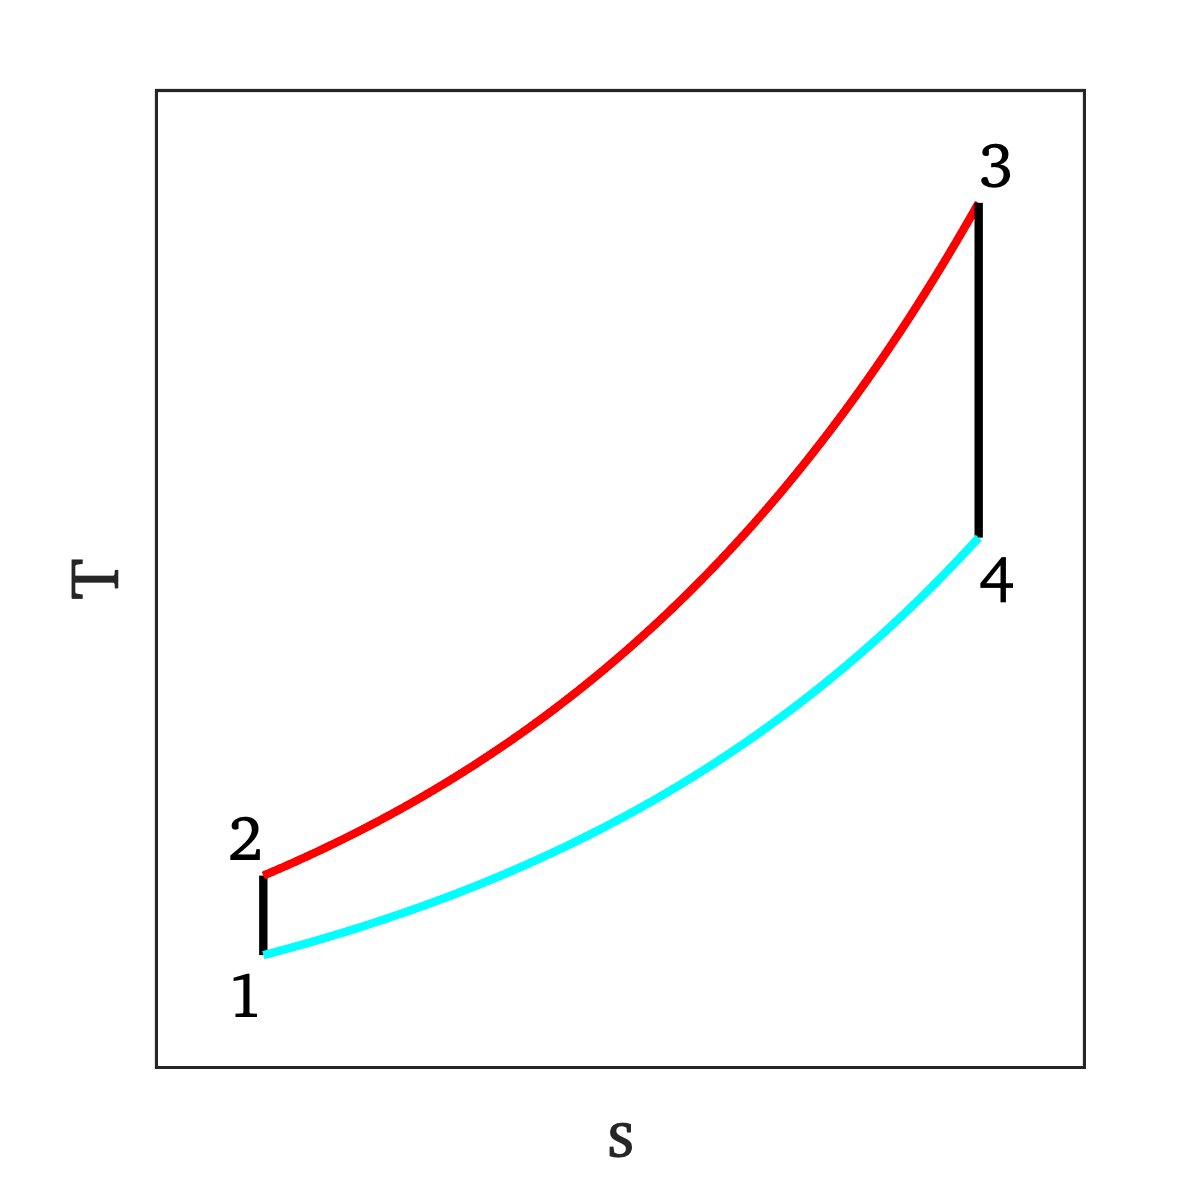
\includegraphics[width=\linewidth]{figs/brayton_cycle_ts_plot.png}
		\caption{T-s plot}
		\label{fig:brayton_cycle_ts_plot}
	\end{subfigure}
	\caption{$p$-$v$ and $T$-$s$ plots of the Brayton thermodynamic cycle}
	\label{fig:brayton_cycle_plots}
\end{figure}

Basic analysis of the ideal Brayton cycle shows that its thermal efficiency is equal to
\begin{equation}
	\eta_{th} = 
	1 - 
	\left(
		\frac{p_{i1}}{p_{i2}}
	\right)
	^
	\frac{\gamma-1}{\gamma}
\end{equation}
where the subscript $i$ denotes that this analysis is of an ideal cycle. For maximum thermal efficiency, it is thus desirable to maximise the pressure increase produced by the engine's compressor, which is responsible for the process of isentropic compression between stations $1$ and $2$. The compression ratio is limited in practice by the pressure increase that is achievable by contemporary compressors, which must balance the goal with the avoidance of stall, the need for a wide range of operating conditions, and the avoidance of excess complexity from adding additional spools. Cruise-condition compression ratio is thus a design specification which sets the value of $p_{i2}$.

The engine's combustor is responsible for the process of isobaric heat addition between stations $2$ and $3$. The rate of heat addition to the flow is given by
\begin{equation}
	Q_{23} = 
	\dot{m_i}
	c_p
	\left(
		T_{i3} - T_{i2}
	\right)
\end{equation}
where $\dot{m_i}$ is the mass flow rate through an ideal engine core. For the purpose of illustration, the influences of bleed and cooling air mass flow rate are not considered, and $\dot{m_i}$ is taken to be the mass flow rate through the engine compressor, combustor, nozzle guide vanes, and turbine. $c_p$ is the specific heat of air at constant pressure and $T_{i2}$ is derived from the compressor inlet temperature $T_{i1}$ via isentropic compression as
\begin{equation}
	T_{i2} = 
	T_{i1}
	\left(
		\frac{p_{i2}}{p_{i1}}
	\right)
	^
	\frac{\gamma-1}{\gamma}
\end{equation}
combining to express the heat added as
\begin{equation}
	Q_{23} = 
	\dot{m_i}
	c_p
	\left[
		T_{i3} - 
		T_{i1}
		\left(
			\frac{p_{i2}}{p_{i1}}
		\right)
		^
		\frac{\gamma-1}{\gamma}
	\right]
\end{equation}
It is desirable to maximise the specific power of the engine in order to build the smallest engine possible. This is achieved by maximising the heat added to the flow, which would result in an increase in in $T_{i3}$. A technological limitation is once again presented: the maximum $T_{i3}$ is limited by the avoidance of overheating the post-combustor nozzle guide vanes, for which heat management is of prime concern to the field. $T_{i3}$ is thus a design specification.

Heat addition is well controlled for in contemporary lean-burn engines, where it may be modelled by the relationship
\begin{equation}
	Q_{23} = 
	\eta_h
	H_{LV}
	\dot{m_f}
\end{equation}
where $\dot{m_f}$ is the fuel mass flow rate, $H_{LV}$ is the lower heating value of jet fuel and $\eta_h$ is a constant to account for inefficiencies of heat addition beyond the scope of the present illustration. The above equations combine to show that the required fuel mass flow rate may be modelled by the expression
\begin{equation}
	\frac{\dot{m_f}}{\dot{m_i}}
	=
	\frac{c_p}{\eta_{h}H_{LV}}
	\left(
		T_{i3} - 
		T_{i1}
		r_p
		^
		\frac{\gamma-1}{\gamma}
	\right)
\end{equation}
where $r_p$ is the compression ratio, $\frac{p_{i2}}{p_{i1}}$. It is shown that the core mass flow rate, $\dot{m_i}$, must be accurately predicted if the engine is to be accurately maintained at the optimal operating conditions allowed by its construction. $r_p$ and $T_{i3}$ are known design specifications, $T_{i1}$ is a measurable ambient condition, and all other terms are approximately constant. 

The design of any jet engine depends on accurate prediction of $\dot{m_i}$. It is shown that this is directly tied to the performance and operational margins of the upstream engine components. Predictability of $\dot{m_i}$ also affects the design of every downstream turbine stage. If it differs from its expected value due to a poor prediction, all subsequent turbine stages will be sized for an incorrect mass flow rate. The resulting errors in flow velocity and pressure will compound with each additional stage, leading to increasingly incorrect specification of turbine sizes and turning angles.

Guiffre' and Pini~\cite{guiffre_design_guidelines} performed numerical analysis to discuss scaleable guidelines for turbine stage design, validating their model using high-fidelity CFD.  Correct stage matching was found to be highly dependent on matching the \textit{volumetric flow ratio}, defined by the authors as a stage's total-to-static density ratio. To accurately quantify this parameter within the analytical and computational methods discussed in this thesis, mass flow rate would need to be predicted correctly.

A strong understanding of NGV mass flow rate predictability should allow engine-makers to pre-empt geometric changes that happen to NGVs during service, such as erosion and cooling hole blockage. It should also account for geometric uncertainties arising from the manufacturing process. While this study advocates for improved accuracy of capacity predictions, emphasis is placed on how these predictions are limited by the unpredictability of real-world manufacture and service.

Section~\ref{flow_capacity_background_definition_and_derivation} will outline the analysis involved in parameterising and predicting mass flow rate. The section will also present the alternative metric of \textit{flow capacity} as a more useful way of characterising mass flow rate independently of the NGV upstream total pressure and temperature. Defining a purely geometric mass flow rate capacity allows for experimental testing of NGVs without recreating the extreme boundary conditions to which real NGVs are exposed. Setting the correct pressure ratio is sufficient, as the subsequent derivation will show. This expedites the testing of different NGV geometries' effects on mass flow rate.

\newpage
\section{Flow capacity: background, definition, and derivation}
\label{flow_capacity_background_definition_and_derivation}

The capacity of an internal combustion engine is an intuitive concept. It is simple to derive from the engine's geometry, it has tangible units of volume, and it provides an heuristic for the engine's size, performance, and air mass flow rate. The design of turbomachinery invites an analogous concept to that of IC engine capacity, but a definition is not so obvious. Mass flow rate through an engine's nozzle guide vane is a function of the NGV's geometry and of its boundary conditions. If the mass flow rate can be quantified in a way which mitigates the boundary conditions, then the effects of an NGV's geometry on its mass flow rate may be isolated. A particular NGV will thus have a mass flow rate capacity, just as a particular IC cylinder has a volumetric capacity.

In 1 dimension, an engine nozzle may be modelled as a compressible flow from an upstream reservoir of total pressure $p_0$, accelerating to velocity $u$ and density $\rho$ through a nozzle of cross-sectional area $A$. Mass flow rate through the nozzle is thus
\begin{equation}
\dot{m} = \rho A u
\end{equation}
where density may be expressed as a function of \textit{pressure ratio}, the ratio of the nozzle pressure to the total pressure
\begin{equation}
\rho = \frac{p_0}{R T_0} \left(\frac{p}{p_0}\right)^\frac{1}{\gamma}
\end{equation}
and velocity is given by conservation of energy as
\begin{equation}\label{compressible_bernouilli}
u =
\sqrt[•]{ 
	2 \left( \frac{\gamma}{\gamma - 1} \right) \left[ \frac{p_0}{\rho_0} - \frac{p}{\rho} \right] 
}
\end{equation}

The above equations combine to express mass flow rate through the nozzle as
\begin{equation}
\dot{m} =
A
\frac{p_0}{R T_0}
\left(\frac{p}{p_0}\right)^\frac{1}{\gamma}
\sqrt[•]{ 
2 \left( \frac{\gamma}{\gamma - 1} \right) 
\left[ \frac{p_0}{ \left( \frac{p_0}{R T_0} \right) } - \frac{p}{ \left( \frac{p_0}{R T_0} \right) \left(\frac{p}{p_0}\right)^\frac{1}{\gamma} } \right] 
}
\end{equation}
which simplifies to
\begin{equation}\label{mass_flow_rate_formula}
\dot{m} =
\frac{p_0}{\sqrt[•]{T_0}} \>
A \;
\sqrt[]{\frac{\gamma}{R}}
\left(
    \frac{p}{p_0}
\right)^\frac{1}{\gamma}
\sqrt[•]{
	\left(
		\frac{2}{\gamma - 1}  
	\right)
	\left[
		1 - \left( \frac{p}{p_0} \right)^\frac{\gamma-1}{\gamma}
	\right] 
}
\end{equation}

Using $\dot{m}$ from Equation~\ref{mass_flow_rate_formula}, capacity is defined as
\begin{equation}\label{capacity_definition}
\Gamma = \frac{\sqrt[•]{T_0}}{p_0}  \>
\dot{m}
\end{equation}
This provides an expression of mass flow rate independent of upstream total pressure $p_0$ and upstream total temperature $T_0$. For isentropic flow, the expression is purely a function of throat area $A$ and pressure ratio $\frac{p}{p_0}$:
\begin{equation}
\Gamma =
A \;
\sqrt[]{\frac{\gamma}{R}}
\left(
    \frac{p}{p_0}
\right)^\frac{1}{\gamma}
\sqrt[•]{
	\left(
		\frac{2}{\gamma - 1}  
	\right)
	\left[
		1 - \left( \frac{p}{p_0} \right)^\frac{\gamma-1}{\gamma}
	\right] 
}
\end{equation}

For throat area $A$ and pressure ratio $r$:
\begin{equation}
\Gamma \left( A, r \right) = 
\sqrt[]{\frac{2\gamma}{R\left(\gamma-1\right)}}
A \;
\sqrt[]{
	r^\frac{2}{\gamma}
	\left(
		1 - r ^\frac{\gamma-1}{\gamma}
	\right) 
}
\end{equation}
This expression has its maximum value at the critical pressure ratio
\begin{equation}
r_c =
\left(
	\frac{\gamma+1}{2}
\right)
^\frac{\gamma}{1-\gamma}
\end{equation}
At lower ratios, the nozzle is choked and mass flow rate cannot increase further. Choked capacity is given by
\begin{equation}
\Gamma_c \left( A \right) =
\sqrt[]{\frac{2\gamma}{R\left(\gamma-1\right)}}
A \;
\sqrt[]{
	\left(
		\frac{\gamma+1}{2}  
	\right)
	^\frac{2}{1-\gamma}
	\left[
		1 - 
		\left(
			\frac{\gamma+1}{2}
		\right)
		^{-1}
	\right]
}
\end{equation}
which simplifies to
\begin{equation}\label{choked_capacity_from_area}
\Gamma_c \left( A \right) =
A \;
\sqrt[]{
	\frac{\gamma}{R}
}
\left(
	\frac{\gamma+1}{2}
\right)
^\frac{1+\gamma}{2\left(1-\gamma\right)}
\end{equation}

It is shown that the capacity of one-dimensional isentropic nozzle flow is a function of only the flow's minimum area, provided the flow is choked and the ratio of specific heats is assumed constant. 

Section~\ref{research_structure} will introduce the structure of the following chapters, which are to analyse the capacity of 2-dimensional and 3-dimensional nozzle flows, presenting and discussing analytical techniques for applying the 1D capacity equation to 2D and 3D data. In such cases, capacity will be defined by equation~\ref{capacity_definition}.


\section{Research structure}
\label{research_structure}

The present study seeks to categorise and examine the ways in which nozzle guide vane flow departs from 1-dimensional compressible flow. These departures are numerous and diverse. The study's scope is to include 2 categories of phenomena: difficulties in predicting the mass flow rate through real nozzle guide vanes, and difficulties in quantifying and modelling the loss incurred by various practical solutions to the need for NGV coolant flow.

Although NGV flow capacity is arguably to be maximised in pursuit of greater power, and loss is certainly to be minimised in pursuit of greater efficiency, it is practical to divide efforts according to the areas of NGV engineering where limitations are present. The present study has identified 3 such areas.
\begin{itemize}
	\item NGV casting processes causing variations in overall shape and throat area, limiting the predictability of flow capacity.
	\item Trailing edge machining processes causing variations in trailing edge shape, resulting in complex variations in the flow field near the downstream extremity of the trailing edge, with corresponding variations in flow capacity.
	\item Sensitivity of flow capacity to the addition of extra film cooling holes on the NGV leading edge suction side, including sensitivity to their exact location.
\end{itemize}

NGVs are cast to high precision. Chapter~\ref{chapter_geometric_throat_area} will present the variations that nonetheless exist among sets of vanes that are intended to be identical. These variations are shown to affect the NGVs' geometric throat area. The chapter discusses the challenges inherent in finding a definition of throat area that usefully predicts the flow capacity of an NGV. The effects of 2-dimensional flow phenomena and geometric variations are presented as confounding factors when considering 2D nozzle flow as opposed to 1D. Further complexity is shown to arise when extending analyses to 3D, where 3D CFD data gathered by Rolls-Royce plc are compared to 2D CFD data from the present study.

Chapter~\ref{chapter_trailing_edge} will discuss the other way in which NGV manufacturing introduces geometric variations that reduce capacity predictability, namely the machining of the trailing edge shape. The machining is designed to optimise the trailing edge's aerodynamics, and not necessarily to minimise variations in its shape. The chapter presents 2D CFD analyses of the effects of variable trailing edge cutback sizing on the 2D flow field and resulting flow capacity of the NGV. To address the variability of contemporary trailing edge designs and to examine the possibility of thicker trailing edges in the event of novel manufacturing methods, the chapter presents 2D CFD analyses of a design without a cutback. This design's loss performance is analysed, informed by a review of various definitions of loss from the literature, where a lack of consensus on a loss definition is demonstrated.

Chapter~\ref{chapter_leading_edge} will analyse the effects of film coolant injection location on both flow capacity and loss. The chapter discusses the possible requirement for an additional suction-side film cooling hole row to be added to NGVs. Given the variability inherent in the process of drilling film cooling holes, justification is given for a 2D CFD study of the effects of hole location on flow capacity and loss, analogous to the variable trailing edge study of Chapter~\ref{chapter_trailing_edge}. A correlation between hole location and flow capacity is analysed, as is the hole location's effect on loss. %The chapter also presents a quasi-3D CFD study to demonstrate that 2D CFD (which amounts to a cooling slot) does not accurately model the discharge and mixing phenomena of a row of circular holes.

Literature is reviewed throughout the thesis whenever relevant to the topic under discussion, rather than a separate chapter.

\section{Summary of findings}

Chapter~\ref{chapter_geometric_throat_area} shows that geometric throat width is a useful predictor of 2-dimensional nozzle guide vane flow capacity. However, the accuracy of the prediction is shown to be dependent on the feasibility of predicting the shape of the sonic line when the NGV is fully choked. If the sonic line is known to not vary significantly in shape within a given production standard of NGV, designers may have more confidence in using the geometric throat area to predict capacity without the use of CFD. In general, capacity predictability is challenged by the reduction of effective throat area by boundary layers whose thickness is difficult to define. Where a sonic line exists, its stability and its approach to the surface may be affected by the presence of the boundary layer. In 3 dimensions, capacity predictability is further challenged by the existence of secondary flows which migrate across the span.

Chapter~\ref{chapter_trailing_edge} shows how changes to the NGV trailing edge geometry affect capacity differently at different pressure ratios. Changes to the NGV suction side trailing edge have little effect at fully-choked pressure ratios, whereas changes to the pressure side have a significant effect at the same pressure ratios. This is shown to result from the relative importance of the throat width when the flow is choked, compared to when it is not. At unchoked pressure ratios, it is possible for post-throat geometric changes to have a significant effect on capacity. The chapter also presents a detailed investigation of the aerodynamic penalties of altering the NGV trailing edge.

Chapter~\ref{chapter_leading_edge} shows that the introduction of film coolant on the NGV suction side has a significant effect on capacity. Coolant injection into locally slower regions is found to have a minimal penalty on both capacity and loss, and in extreme cases to even increase the capacity. Coolant injection into locally faster regions is found to cause a reduction in the capacity. The coolant injection is argued to be equivalent to a change in the effective area at the point of injection, which is in agreement with the arguments about effective area presented in the earlier chapters.

The overall work thus provides insight into the necessary geometric parameters for an initial 2D aerofoil design, showing which parameters require iterative calculation and which may be changed without significant penalty to capacity or aerodynamics.



\chapter{Geometric throat area}
\label{chapter_geometric_throat_area}
%this chapter is about the definition of throat area and how to measure it

% NEEDED DATA:
% -T900 smooth vanes, 6x 2D CFD solutions at various pressure ratios
% -Not sure where the 3D data came from, can we check this? ie --GOM scan data

%plan for chapter - answer the following questions:
% 1) what does "throat area" MEAN beyond 1D? Is it the smallest area across the nozzle, or is it a line/surface drawn according to real flow features, most likely the M1 line?
% 1) why does it work quite well in 2D, ie what is mostly NOT changing between the geometries (could almost say what is incidentally being controlled for)?
% 2) what starts changing in 3D to the extent that no linear signal is recognisable in the noise?

%the raw data consists of: 
% -some 2D vanes with different geometries, and a bunch of 3D vanes with different geometries. Range of PRs. For each, there is a "throat area".
%it is thus possible to plot: 
% -changes in throat area versus changes in capacity for the 2D family, for any given PR
% -changes in throat area versus changes in capacity for the 3D family, for any given PR
% -capacity trends for the 2D and 3D vanes
%for each solution, it is possible to define:
% -a "true throat area" based on the M1 line being crossed at oblique angles by every streamline
% -certain geometric parameters describing how its shape is different to the shape of its other family members

%"throat area" just means the smallest line or surface that can be drawn in a nozzle - not sympathetic to anything actually happening in the flow. It only really works in 1D.

A 1-dimensional supersonic nozzle is equivalent to a single streamline of variable cross-sectional area. It is possible to solve for the flow conditions throughout the nozzle, provided area is specified as a function of position along the nozzle. The mass flow rate capacity is a function of only the flow's minimum area, as in equation~\ref{choked_capacity_from_area}.

A 2-dimensional isentropic fully choked nozzle may be modelled as a group of adjacent streamlines, each of which may have dissimilar area functions. It is notable that the streamlines' minimum areas may not correspond to a straight line across the narrowest part of the nozzle. This is illustrated in Figure~\ref{fig:illustration_of_minimum_area} by supposing the division of a 2-dimensional flow into a finite number of streams of finite width. Each stream has an individual point of minimum width where sonic conditions exist, shown as the transition between subsonic flow in blue and supersonic flow in yellow. These sonic points are distributed on a line distinct from the overall passage line of minimum width. The resulting minimum area line is shown in red along with the geometric minimum area line, to illustrate their disparity.

If this concept is extended to infinitesimal streamlines (and the flow is isentropic) each streamline will experience sonic conditions at its point of minimum area, coalescing to form the 2-dimensional sonic line. The effective throat area of a 2-dimensional nozzle is thus the sum of its streamlines' throat areas. This is distinct from the sonic line length, and may be expressed by the integral
\begin{equation}\label{effective_throat_area_integral}
	A_{eff} = 
	\int_{1}^2 \vu*{u} \vdot \vu*{r} dL
\end{equation}
where $\vu*{u}$ is the unit vector of local flow velocity, $\vu*{r}$ is the unit vector perpendicular to the local sonic line, and the integral is performed on the scalar infinitesimal $dL$ over the length of the sonic line, as illustrated in Figure~\ref{fig:illustration_of_equivalent_throat_area_integral}.
 		
\begin{figure}[H]
	\centering
	\begin{subfigure}{.45\textwidth}
		\centering
		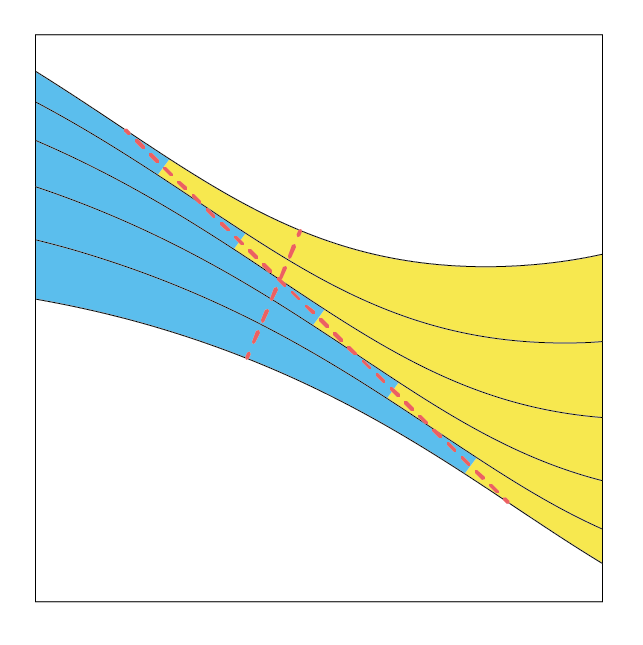
\includegraphics[width=\linewidth]{figs/illustration_of_minimum_area_ver04.png}
		\caption{Different minimum area points of dissimilar streams}
		\label{fig:illustration_of_minimum_area}
	\end{subfigure}
	\hspace{0.05\textwidth}
	\begin{subfigure}{.45\textwidth}
		\centering
		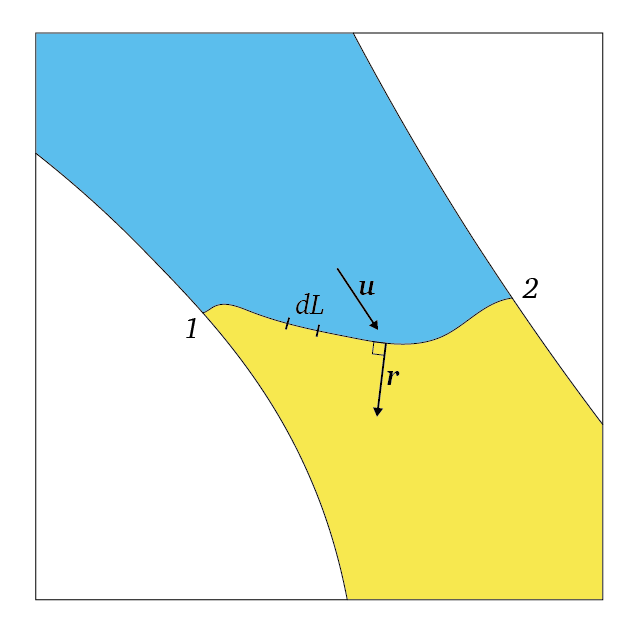
\includegraphics[width=\linewidth]{figs/illustration_of_equivalent_throat_area_integral_ver03.png}
		\caption{Integral for 2D nozzle equivalent throat area \hfill \break}
		\label{fig:illustration_of_equivalent_throat_area_integral}
	\end{subfigure}
	\caption{Considerations for defining the minimum area of an arbitrarily shaped nozzle in choked compressible isentropic flow, where blue areas lie upstream of each stream tube throat and yellow downstream}
\end{figure}

In the case of 1-dimensional nozzle flow, Equation~\ref{effective_throat_area_integral} collapses to the value of the throat area. In the case of 2D flow through an arbitrarily shaped nozzle such as a gas turbine nozzle guide vane, the integral describes the infinitesimal sum of the areas encountered by each streamline at the point of sonic conditions. It is proposed as a physically sensible 2D extension of the 1D concept of throat area, as opposed to finding the narrowest point across the passage to obtain a geometric throat area. 

For a fully choked streamline, flow conditions upstream of the sonic line are independent of those downstream. This facilitates an analytical approach where the flow conditions immediately upstream of any choked streamline's sonic point are treated as a known state. That streamline's mass flow rate is wholly a function of that state, thus the mass flow rate of a fully choked 2D nozzle is wholly a function of its $A_{eff}$ as derived from its sonic line. For an unchoked streamline, its mass flow rate is a function of the state of every point along the streamline, including points downstream of where sonic conditions would appear in choked cases. It is thus advantageous to supplement design-condition simulations with simulations at a pressure ratio where the nozzle guide vane is guaranteed fully choked, allowing for analysis of a fully-formed sonic line and computation of a corresponding $A_{eff}$.

The present study will nonetheless discuss the reasons for which geometric throat area remains a useful predictor of NGV flow capacity in many cases, as has been noted in the literature. Thirumurthy et al~\cite{thirumurthy_throat_area} discussed the challenges and uncertainties associated with the accurate matching of an aeroderivative gas generation turbine. The authors' focus was on various means of predicting capacity to facilitate proper matching. The authors noted that ``the throat area of any blade or vane row has a strong influence on the overall capacity of the turbine. The vane or blade throat plane...is defined as the plane formed by the smallest passage area normal to the flow path. The effects are of first order when the throat area is changed for the first stage of the turbine.'' The prior discussion of effective area is in agreement with this statement. If 2D nozzle throat width is varied in a way that does not significantly affect the sonic line shape, effective area and thus choked mass flow rate would be expected to vary to first order. This hypothesis is tested in this chapter.


\section{Nozzle guide vane capacity uncertainty in 2 dimensions}
\label{section_1d_vs_2d_capacity_uncertainty}
%do I have the T900 family at various PRs, or just at the choking PR? Do I actually need other PRs anyway, given that the throat area stuff looks at the vanes when they are choked?
%I have the case files for just the choked conditions, apparently. But this is ok because I have the gamma curves and plots etc, so I can still enhance the thesis by adding some CFD visualisations at choked conditions, showing the M1 line.
%The point is to see how the different NGVs' capacity varies when plotted against various definitions of throat area. The usefulness of each definition will be discussed.

The immediate challenge in quantifying 2D nozzle flow capacity is that analytical approaches are incomplete. If any nozzle's $A_{eff}$ could be inferred from its geometry, it would be possible to investigate the effects of the geometry on the flow capacity to a high degree of accuracy, but the only way to find $A_{eff}$ is to solve the flow computationally to obtain the sonic line. Once a CFD solution has been obtained, the flow capacity is necessarily also obtained. 

Those concerned with mapping NGV geometry onto flow capacity are thus presented with 2 options: either perform CFD on every conceivable shape of NGV and create a lookup table of arbitrary fidelity, or analyse a relatively small set of CFD solutions to create heuristics about what types of geometric changes cause what types of changes to the shape of the sonic line and local flow vectors. Furthermore, a typical starting point for a commercial engine designer is to conduct a 2D analysis based on a previous ``successful'' engine design, with some cooling features included. This has necessarily limited design changes, and has led to local optimisation within a very small design envelope.

\subsection{Geometry, mesh, and boundary conditions}

Rolls-Royce plc have provided the present study with a family of NGV geometries suitable for such an approach, all from the Trent 900 engine. Geometric variation among Trent 900 NGVs has been subject to extensive measurement by Rolls-Royce. In one such set of studies, Hall~\cite{hall_area} and Zamboni~\cite{zamboni_area} produced geometric definitions of 6 NGVs. These 6 NGVs are members of 2 slightly different production standards within the Trent 900 NGV family, which are referred to by the company as the M-skew standard and the EP1 standard. Rolls-Royce randomly selected three production NGVs from each standard and measured their surface geometries using the \textit{white light}/\textit{GOM} scanning method. This resulted in the 6 geometric definition files used by Hall~\cite{hall_area} and Zamboni~\cite{zamboni_area}, which were provided to the present study. These files do not include film cooling holes or the trailing edge slot. The trailing edges are smoothly rounded.

Variations exist among the geometry of the 6 NGVs, even when cooling features are not accounted for. Although these variations are of the order of $0.5$ mm, they are sufficiently large to significantly affect flow capacity. Zamboni~\cite{zamboni_area} described the process for quantifying these variations in 3D, which will be discussed in Section~\ref{2d_vs_3d_capacity_uncertainty}. The present study defined an approach for deriving 2D geometries from the 3D files and quantifying the variations among them.

The 3D NGV surface shape was provided by Rolls-Royce as a set of co-ordinates which define 21 closed loops on the vane surface. Each loop consists of a pair of streamlines which diverge from a stagnation point on the vane's leading edge and converge at the trailing edge. The 11th loop was thus considered to be the closest approximation to a mid-span slice of the NGV. MATLAB was used to process the 3D curve of the 11th loop, producing a 2D section via the following process. 
\begin{enumerate}
  \item Project the loop's coordinates onto a cylindrical surface whose radius is equal to the NGV annular radius at mid-span.
  \item Periodically repeat the resulting shape in the circumferential direction to create an annulus of 2D vanes wrapped around the cylinder.
  \item Transform the annulus into an infinite 2D linear cascade by taking the circumferential coordinate to be a vertical coordinate.
\end{enumerate}
This process is illustrated in Figure~\ref{fig:2d_geometry_creation}.

\begin{figure}[H]
	\centering
	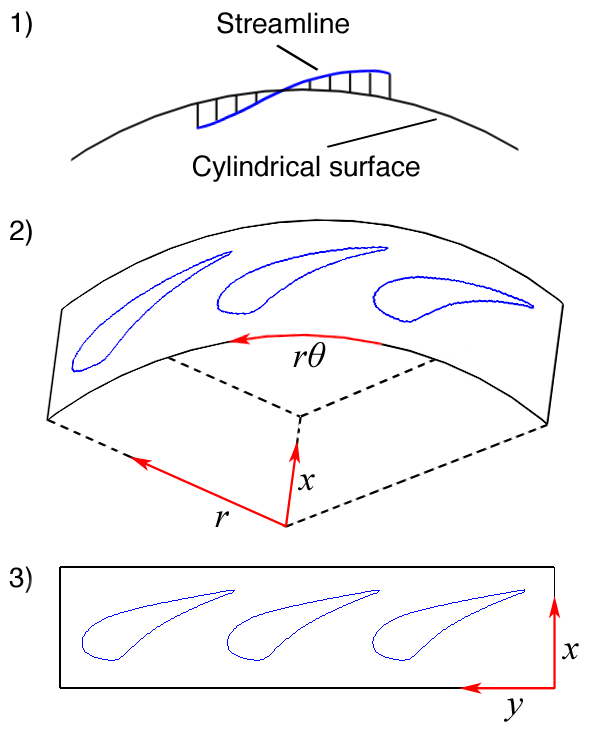
\includegraphics[width=.6\textwidth]{figs/2d_geometry_creation.png}
	\caption{Creation of a 2D mid-span approximation of NGV geometry}
	\label{fig:2d_geometry_creation}
\end{figure}

The resulting coordinates were connected to form a closed body. This body was placed in a computational domain consisting of a straight inlet section, a curved turning section, and a straight outlet section inclined at the NGV turning angle. The domain was modelled in Ansys Fluent, where the inlet boundary was specified to have total pressure $p_{01}$ and the outlet boundary was specified to have static pressure $p_2$. The remaining domain boundaries were made periodic with one another to preserve the 2D linear cascade. The NGV surface boundary was specified as a solid wall with a no-slip boundary condition and no heat conduction. The resulting computational domain is illustrated in Figure~\ref{fig:computational_domain_and_boundaries}. On the outlet boundary, labels $0$ and $1$ denote the start and end points for the wake surveys that will be presented in Chapter~\ref{chapter_trailing_edge}.

\begin{figure}[H]
	\centering
	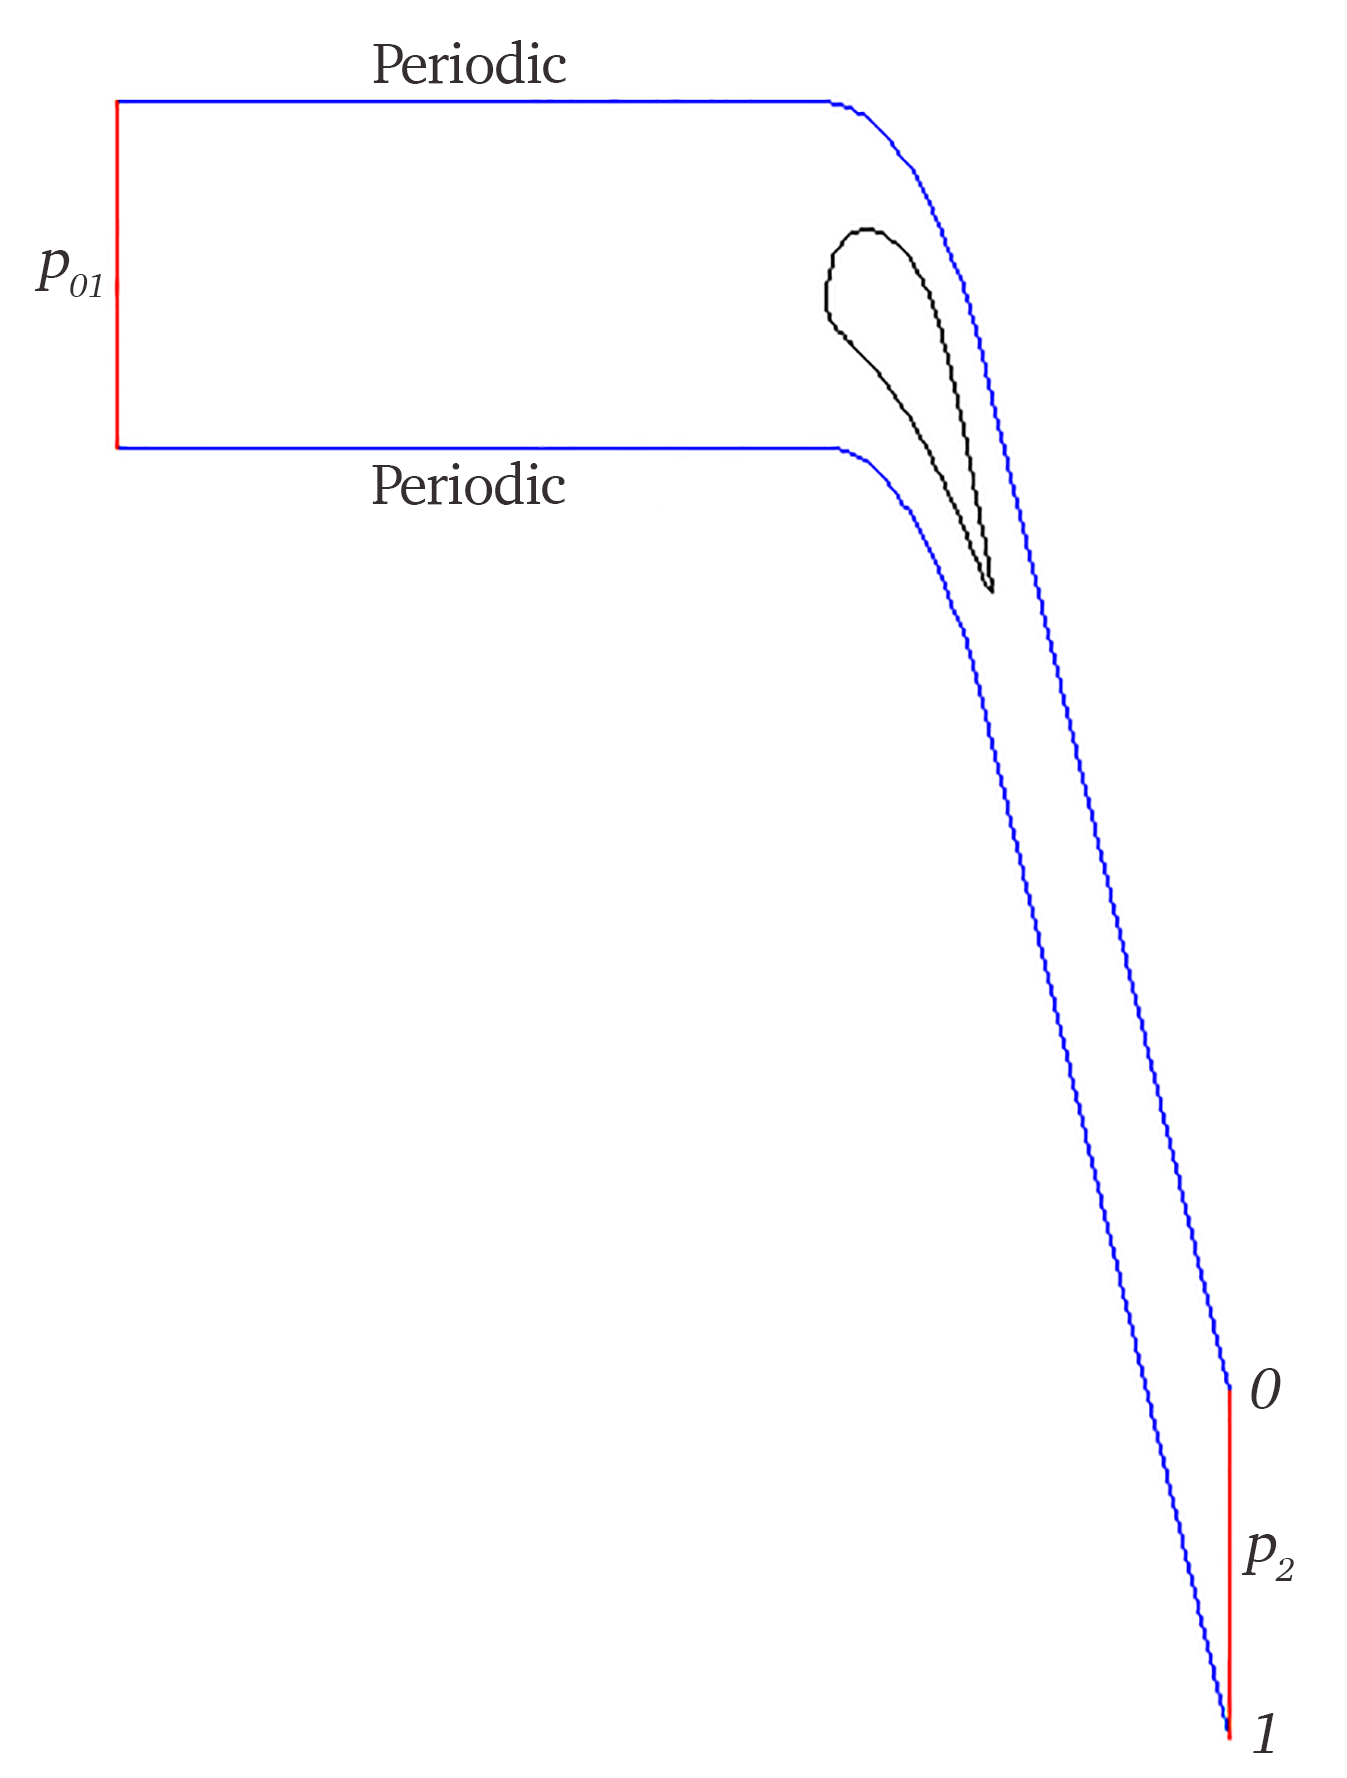
\includegraphics[width=.6\textwidth]{figs/domain_boundary_conditions.png}
	\caption{Domain and boundaries for the present 2D CFD study}
	\label{fig:computational_domain_and_boundaries}
\end{figure}

This configuration has been the basis for all other 2D CFD analyses in this thesis, where additional boundaries are added to account for cooling features as required. Values for the simulation were set according to Table~\ref{T900_parameters}.

% this table's PR checks out. The crazy high pressure ratio on Fluent is just where it finished after going through all the ratios.
\begin{table}[H]
\caption{Boundary conditions at design pressure ratio for Trent 900 multi-vane capacity study}
\label{T900_parameters}
\begin{center}
\begin{tabular}{|c|c|}
\hline
Parameter & Value\\
\hline
NGV series & Rolls-Royce Trent 900\\
NGV turning (degrees) & $76.89$\\
Inverse pressure ratio $\frac{p_{01}}{p_2}$ & $1.79$, $3.33$\\
Inlet total pressure (Pa) & $4.33 \times 10^6$\\
Inlet total temperature (K) & $300$\\
Outlet static pressure (design) (Pa) & $2.42 \times 10^6$\\
Outlet static temperature (K) & $300$\\
Solver type & Density-based\\
Cell count & $35,000$\\
\hline
\end{tabular}
\end{center}
\end{table}

For turbomachinery flows of this type, the boundary layer thickness will be shown to be large enough to significantly affect the NGV throat area. The mesh must resolve the whole boundary layer within a region of high resolution which is sufficiently large to cover the maximum boundary layer thickness. The maximum thickness of a turbulent boundary layer is approximated by the formula
\begin{equation}\label{boundary_layer_thickness}
\delta \approx
0.37
\frac{L}{Re^\frac{1}{5}}
\end{equation}
where $L$ is the characteristic length in the direction of the flow (the approximate NGV chord length) and $Re$ is the Reynolds number. The Reynolds number is defined as
\begin{equation}
Re = 
\frac{uL\rho}{\mu}
\end{equation}
where $u$ is a representative value for flow velocity and $\mu$ is the dynamic viscosity of the fluid within the temperature range of the flow. For compressible flow, the velocity and density are substituted to give
\begin{equation}
Re = 
\frac{
	M\sqrt{\gamma RT}L\frac{p}{RT}
}{
	\mu
}
\end{equation}
For isentropic flow, this may be expressed in terms of total temperature and pressure as
\begin{equation}\label{reynolds_number_compressible}
Re = 
\frac{L}{\mu}
\sqrt{\frac{\gamma}{R}}
\frac{p_0}{\sqrt{T_0}}
M
\left(
	1 +
	\frac{\gamma-1}{2}
	M^2
\right)
^{\frac{\gamma+1}{2(1-\gamma)}}
\end{equation}

Equation~\ref{reynolds_number_compressible} was used to compute a Reynolds number for the case of choked or near-choked NGV flow with the following values, based on the values specified in Table~\ref{T900_parameters}.
\begin{table}[H]
\caption{Values for computing an approximate Reynolds number for an NGV passage}
\label{reynolds_number_parameters}
\begin{center}
\begin{tabular}{|c|c|}
\hline
Parameter & Value\\
\hline
$L$ & 0.08 m\\
$\mu$ & $19 \times 10^{-6}$ Pas\\
$p_0$ & $4.33 \times 10^6$ Pa\\
$T_0$ & 300 K\\
$\gamma$ & 1.4\\
$R$ & 287 Jkg$^{-1}$K$^{-1}$\\
$M$ & 1\\
\hline
\end{tabular}
\end{center}
\end{table}
This resulted in a value of $Re = 4.2 \times 10^7$. Maximum boundary layer thickness was thus estimated using equation~\ref{boundary_layer_thickness} to be 1 mm. This is of the order of 10\% of the NGV throat width, so full resolution of the boundary layer is required for any CFD study of the effects of NGV geometric changes.

The NGV surface was enclosed in a structured quadrilateral mesh which extended out by 2 mm. Compared to the estimated maximum boundary layer thickness, the factor of 2 ensured that the whole boundary layer was captured, reduced the gradient of cell size change within the boundary layer mesh, and provided additional resolution within the base region downstream of the trailing edge, where boundary layer separation and entropy generation occur amid high surface curvature.

Full resolution of the boundary layer required placement of mesh elements within the laminar sub-layer. Regions within the boundary layer were assumed to be divided according to the \textit{universal law of the wall}. This boundary layer model is derived from experimental measurements and dimensional analysis performed by Nikuradse~\cite{nikuradse_boundary_layers}. The author's motivation was the need to predict the velocity profile and thickness of turbulent boundary layers, given the free-stream conditions. The work is of renewed importance in the context of contemporary CFD such as the present study, where knowledge of appropriate boundary layer mesh resolution is mandatory. 

Nikuradse~\cite{nikuradse_boundary_layers} showed that turbulent boundary layers in general exhibit a high degree of dimensional similarity if distance from the wall $y$ is appropriately non-dimensionalised. The assumption was that qualitatively distinct regions of the boundary layer may be characterised by a dimensionless number that takes the place of $y$. Regions closer to the wall are expected to be dominated by viscous forces, and regions closer to the free-stream are expected to be dominated by inertial forces. The dimensionless wall distance parameter is thus expected to take similar form to the Reynolds number. It is defined as
\begin{equation}\label{y_plus}
y_+ =
\frac{u_f y \rho}{\mu} 
\end{equation}
where $u_f$ is the friction velocity, defined as
\begin{equation}\label{friction_velocity}
u_f = 
\sqrt{
	\frac{\tau_w}{\rho}
}
\end{equation}
where $\tau_w$ is the shear stress at the wall boundary. Equation~\ref{friction_velocity} thus characterises the wall shear stress as a velocity which is used in the Reynolds-type formulation of Equation~\ref{y_plus}. $\tau_w$ is defined as
\begin{equation}\label{wall_shear_stress_definition}
\tau_w =
\frac{1}{2}
C_f
\rho
u^2
\end{equation}
where $C_f$ is a coefficient of skin friction and $u$ is the free-stream velocity. $C_f$ may be computed from the free-stream Reynolds number according to the correlation proposed by Schlichting~\cite{schlichting_boundary_layer_theory}
\begin{equation}
C_f =
\left(
	2
	\log_{10}
	Re
	-
	0.65
\right)^{-2.3}
\end{equation}

For isentropic compressible flows, equation~\ref{wall_shear_stress_definition} may be expressed as
\begin{equation}
\tau_w =
\frac{1}{2}
C_f
\frac{p}{RT}
M^2
\gamma
RT
\end{equation}
\begin{equation}
\tau_w =
\frac{1}{2}
C_f
\gamma
p_0
M^2
\left(
	1 +
	\frac{\gamma-1}{2}
	M^2
\right)
^{-\frac{\gamma}{\gamma-1}}
\end{equation}
allowing a compressible expression of $u_f$ as
\begin{equation}
u_f = 
\sqrt{
	\frac{
		\frac{1}{2}
		C_f
		\gamma
		p_0
		M^2
		\left(
			1 +
			\frac{\gamma-1}{2}
			M^2
		\right)
		^{-\frac{\gamma}{\gamma-1}}
	}{
		\rho_0
		\left(
			1 +
			\frac{\gamma-1}{2}
			M^2
		\right)
		^{-\frac{1}{\gamma-1}}
	}
}
\end{equation}
\begin{equation}
u_f = 
\sqrt{
	\frac{
		C_f
		\gamma
		R
		T_0
		M^2
	}{
		2 +
		\left(\gamma-1\right)
		M^2
	}
}
\end{equation}
and allowing a compressible expression of $y_+$ as
\begin{equation}
y_+ = 
\sqrt{
	\frac{
		C_f
		\gamma
		R
		T_0
		M^2
	}{
		2 +
		\left(\gamma-1\right)
		M^2
	}
}
\frac{y}{\mu}
\frac{p_0}{R T_0}
\left(
	1 +
	\frac{\gamma-1}{2}
	M^2
\right)
^{-\frac{\gamma}{\gamma-1}}
\end{equation}
\begin{equation}\label{y_plus_compressible}
y_+ =
\frac{y}{\mu}
\sqrt{\frac{\gamma}{R}}
\frac{p_0}{\sqrt{T_0}}
\sqrt{\frac{C_f}{2}}
M
\left(
	1 +
	\frac{\gamma-1}{2}
	M^2
\right)
^{\frac{\gamma+1}{2(1-\gamma)}}
\end{equation}
This expression is of similar form to the expression for Reynolds number in equation~\ref{reynolds_number_compressible}. Both are shown to be a function of Mach number and of the upstream conditions $\frac{p_0}{\sqrt{T_0}}$. If these expressions are normalised against the upstream conditions in a similar way to flow capacity, it is shown that both the dimensionless speed $Re$ and the dimensionless boundary layer thickness $y_+$ are purely functions of Mach number and of a geometric parameter -- $L$ and $y$ respectively. This is subject to the assumptions that $\mu$ is approximately constant within the range of temperatures and $\sqrt{\frac{C_f}{2}}$ is approximately constant for sufficiently high Reynolds numbers.

Equation~\ref{y_plus_compressible} may be rearranged to compute a real distance $y$ from the wall given a value of $y_+$. In the general case of turbulent boundary layers, the laminar sublayer occupies the region of $y_+ < 5$. The present study placed the first layer of mesh nodes at a wall distance of $0.3$ $\mu$m corresponding to a $y_+$ value of $5$. This is in accordance with a study of laminar sublayer resolution by Salim and Cheah~\cite{salim_y_plus}. The size of the first layer of mesh nodes was confirmed by measurement of the mesh after generation.

Within the structured boundary mesh, element size was grown so that the outermost elements had an aspect ratio of approximately $\frac{1}{2}$. Beyond this, the domain was populated with an unstructured quadrilateral-dominant mesh. Node distributions along the two periodic boundaries were made identical, and nodes adjacent to the structured boundary layer mesh were made to match its outermost node distributions. Within the general domain, unstructured mesh generation was automated using Ansys Fluent's built-in meshing feature. The resulting mesh formed the basis for all other 2-dimensional NGV meshes in the study. The mesh and periodic pattern are depicted in Figure~\ref{fig:t900_mesh_whole} and details of the mesh, showing the structured boundary layer treatment, are depicted in Figure~\ref{fig:t900_mesh_details}.

\begin{figure}[H]
      \centering
      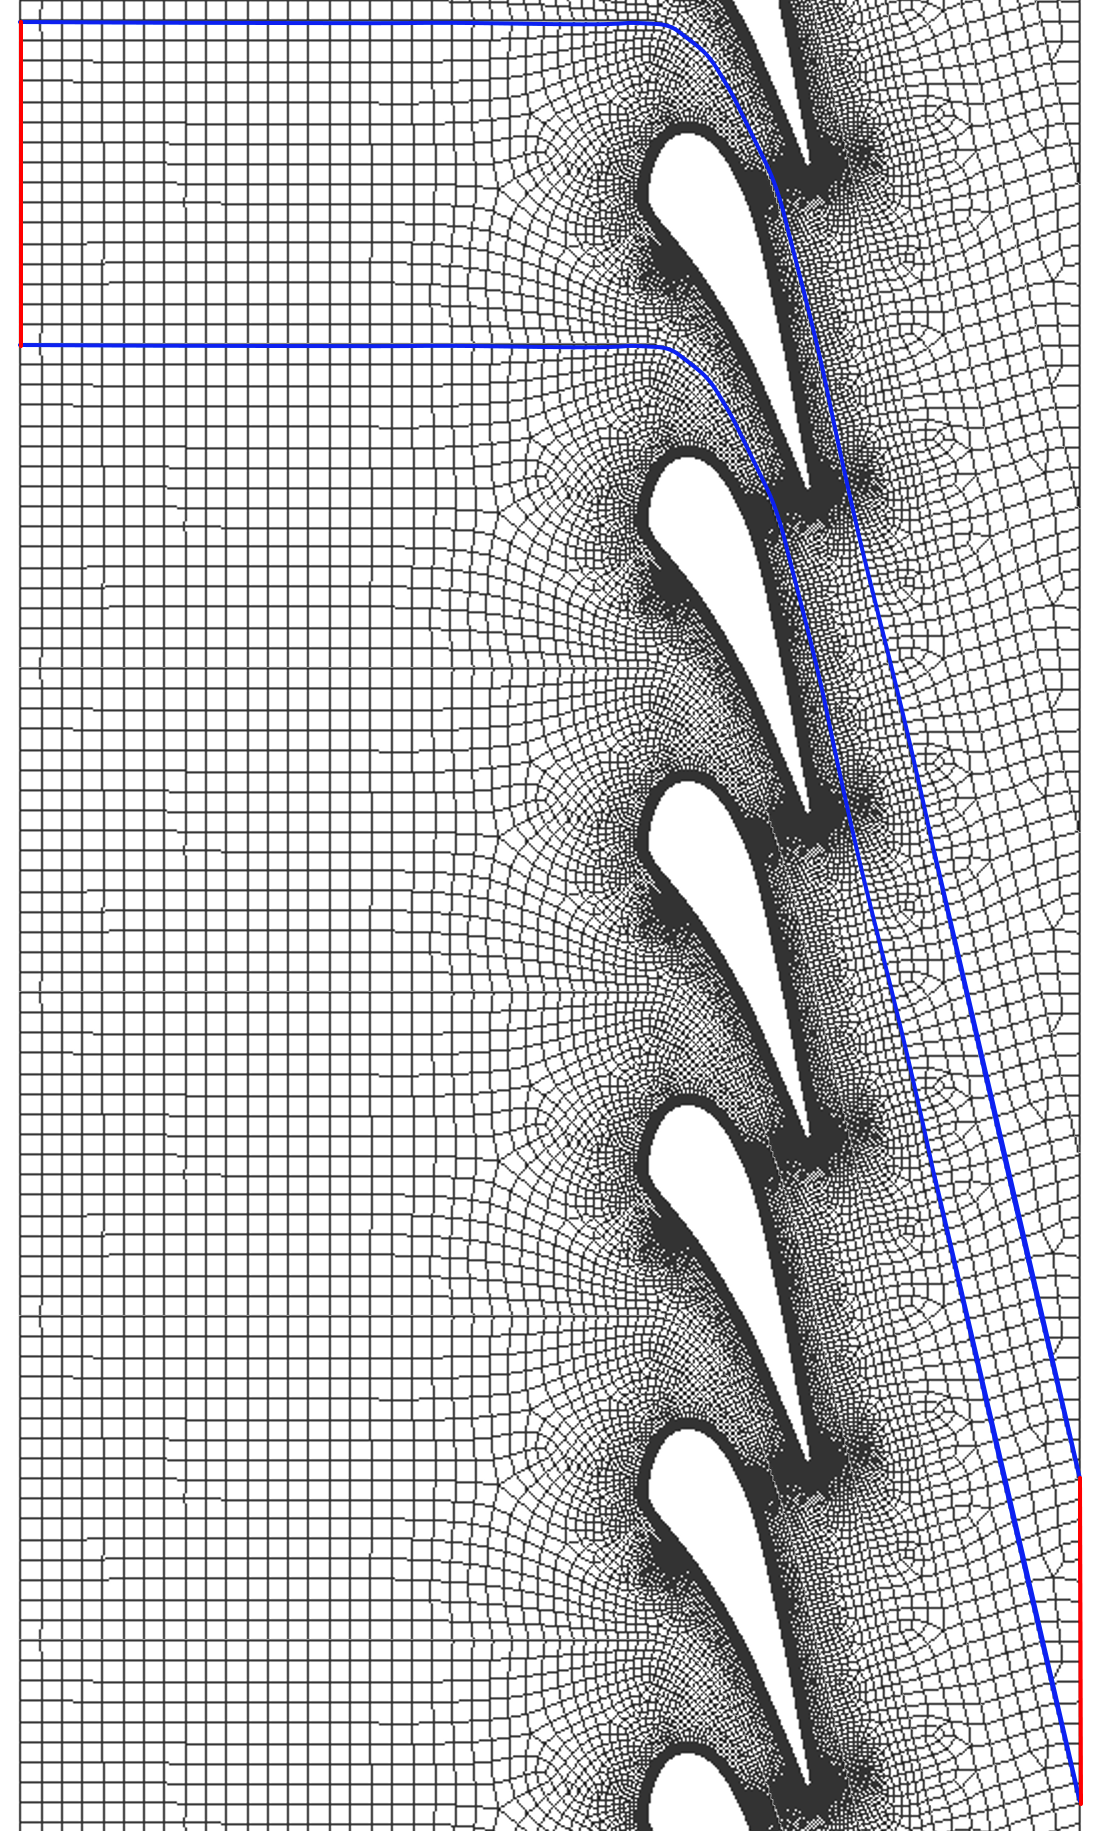
\includegraphics[width=.85\textwidth]{figs/t900_mesh_whole.png}
      \caption{Mesh for Trent 900 throat width variation study, inlet and outlet boundaries shown in red, periodic boundary shown in blue}
      \label{fig:t900_mesh_whole}
\end{figure}

\begin{figure}[H]
	\centering
	\begin{subfigure}{.45\textwidth}
		\centering
		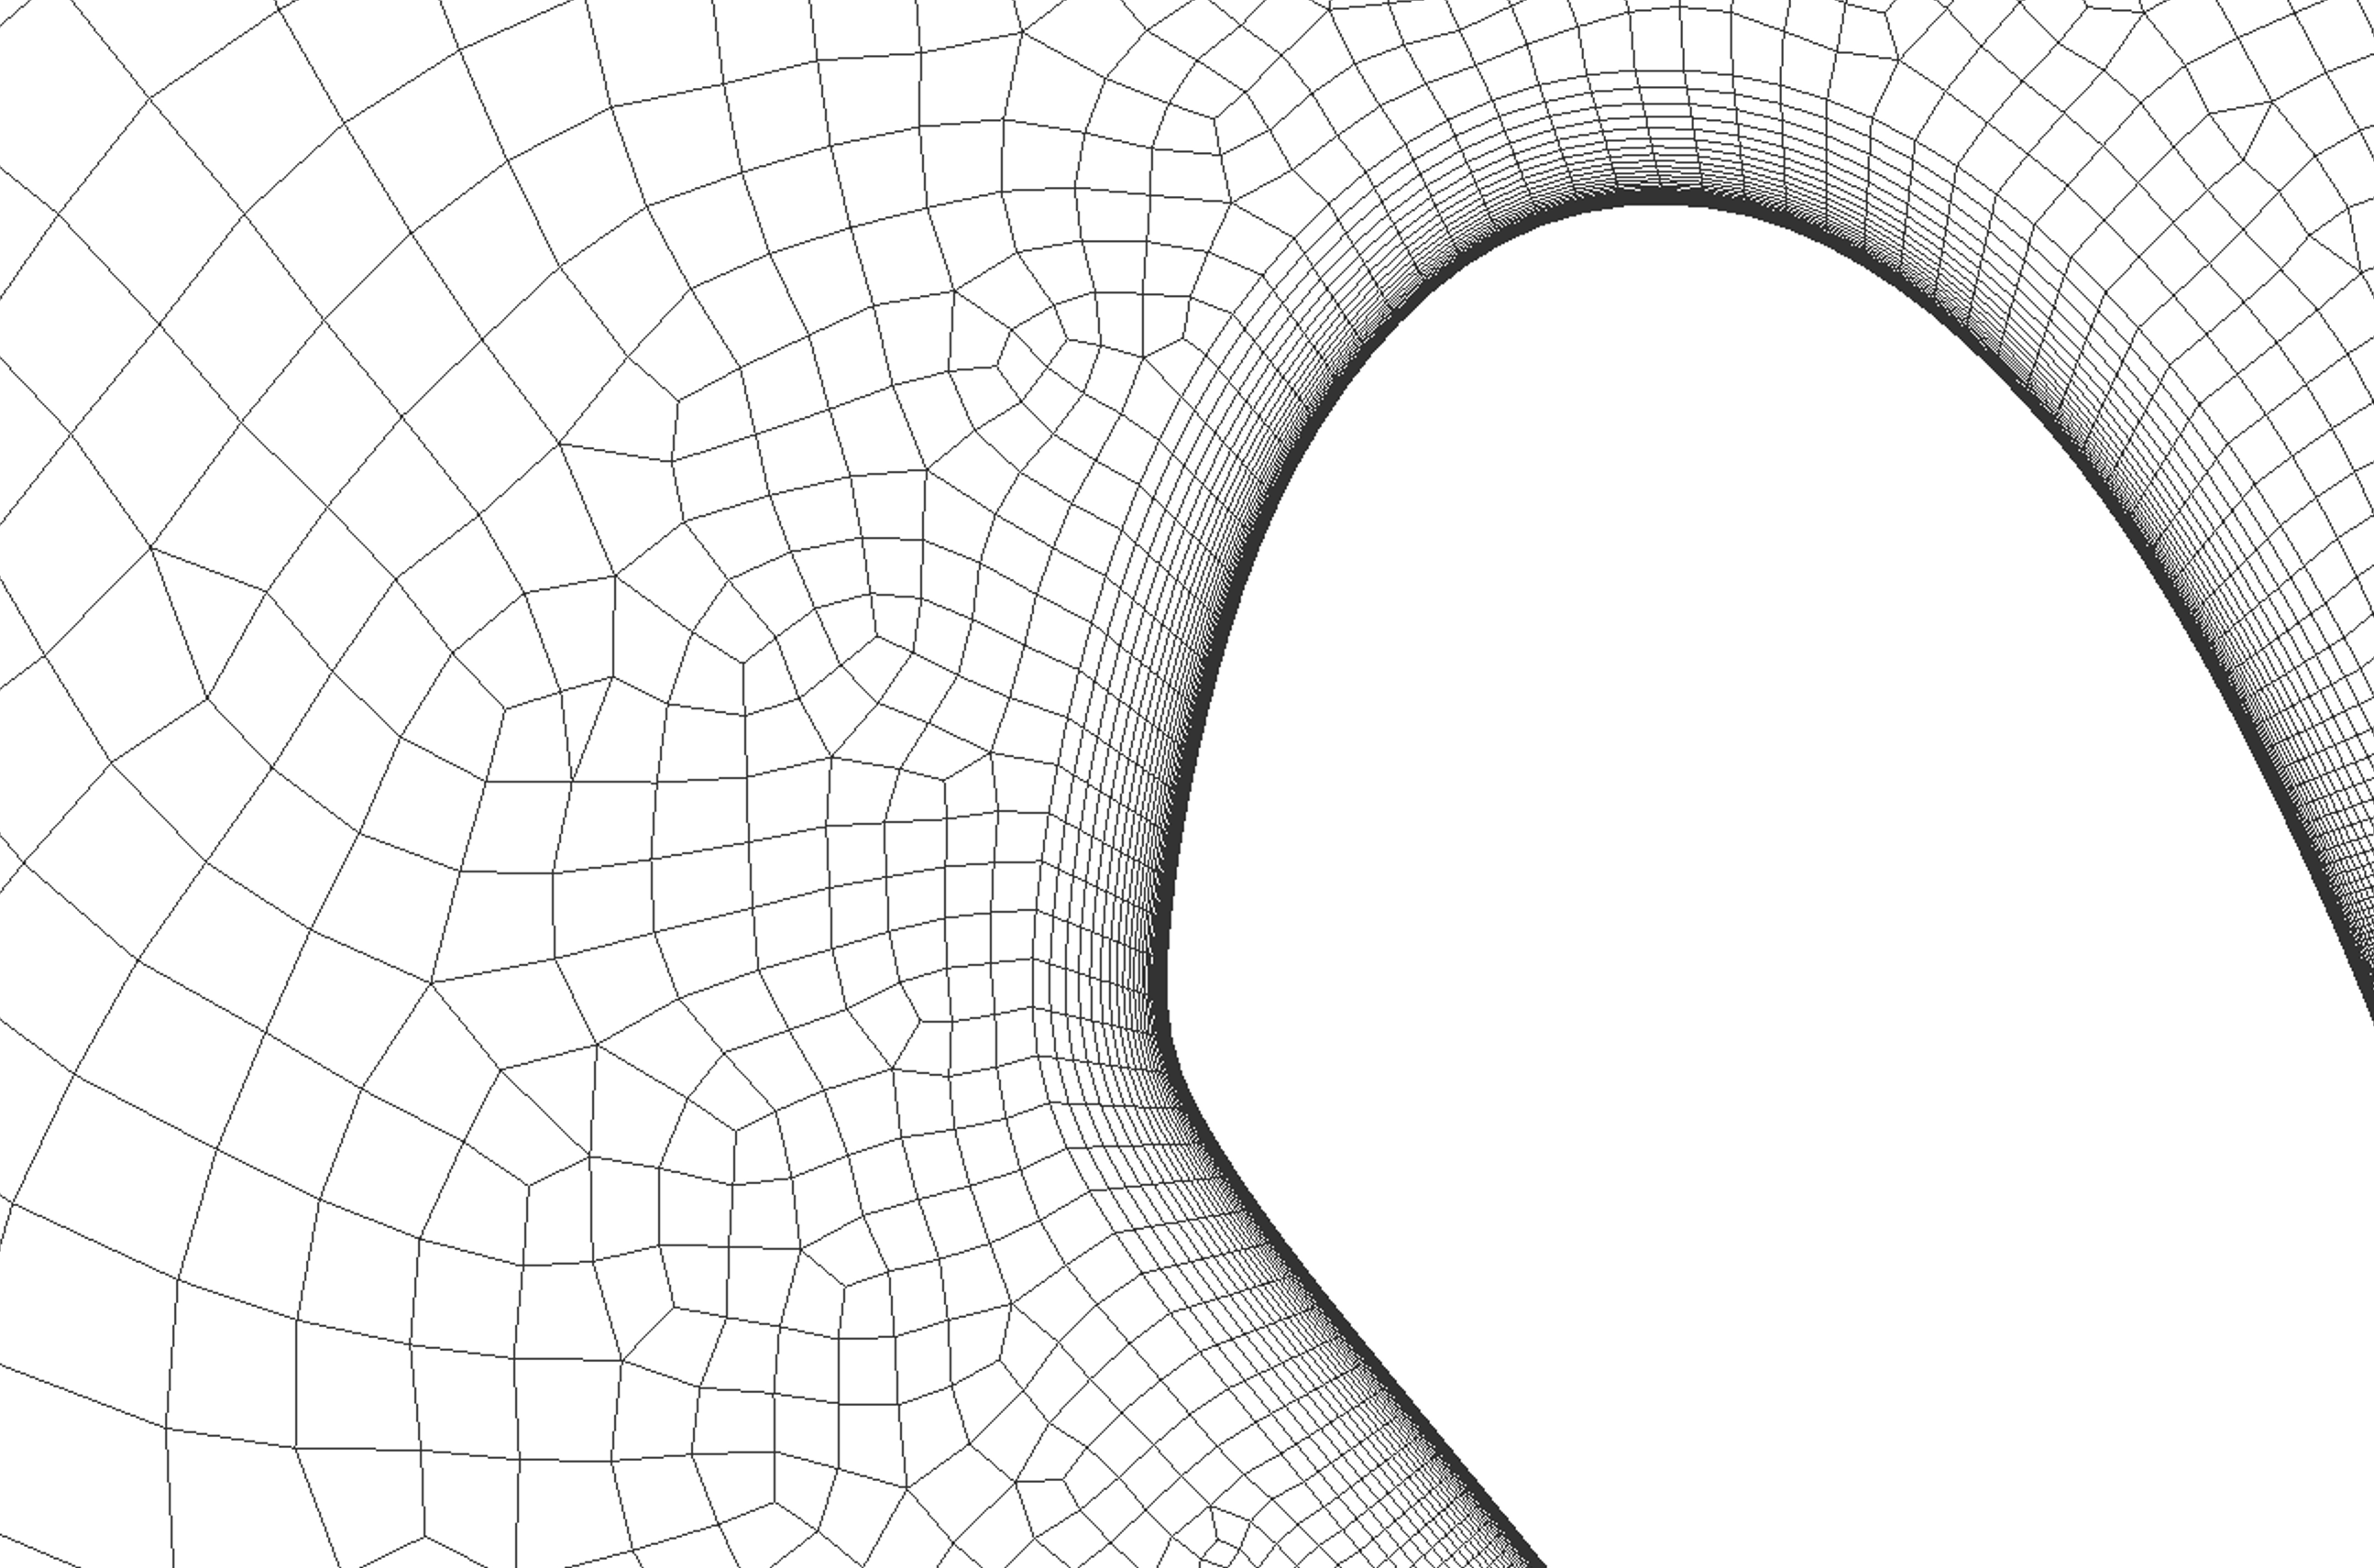
\includegraphics[width=\linewidth]{figs/t900_mesh_leading_edge.png}
		\caption{Leading edge}
		\label{fig:t900_mesh_leading_edge}
	\end{subfigure}
	\hspace{0.05\textwidth}
	\begin{subfigure}{.45\textwidth}
		\centering
		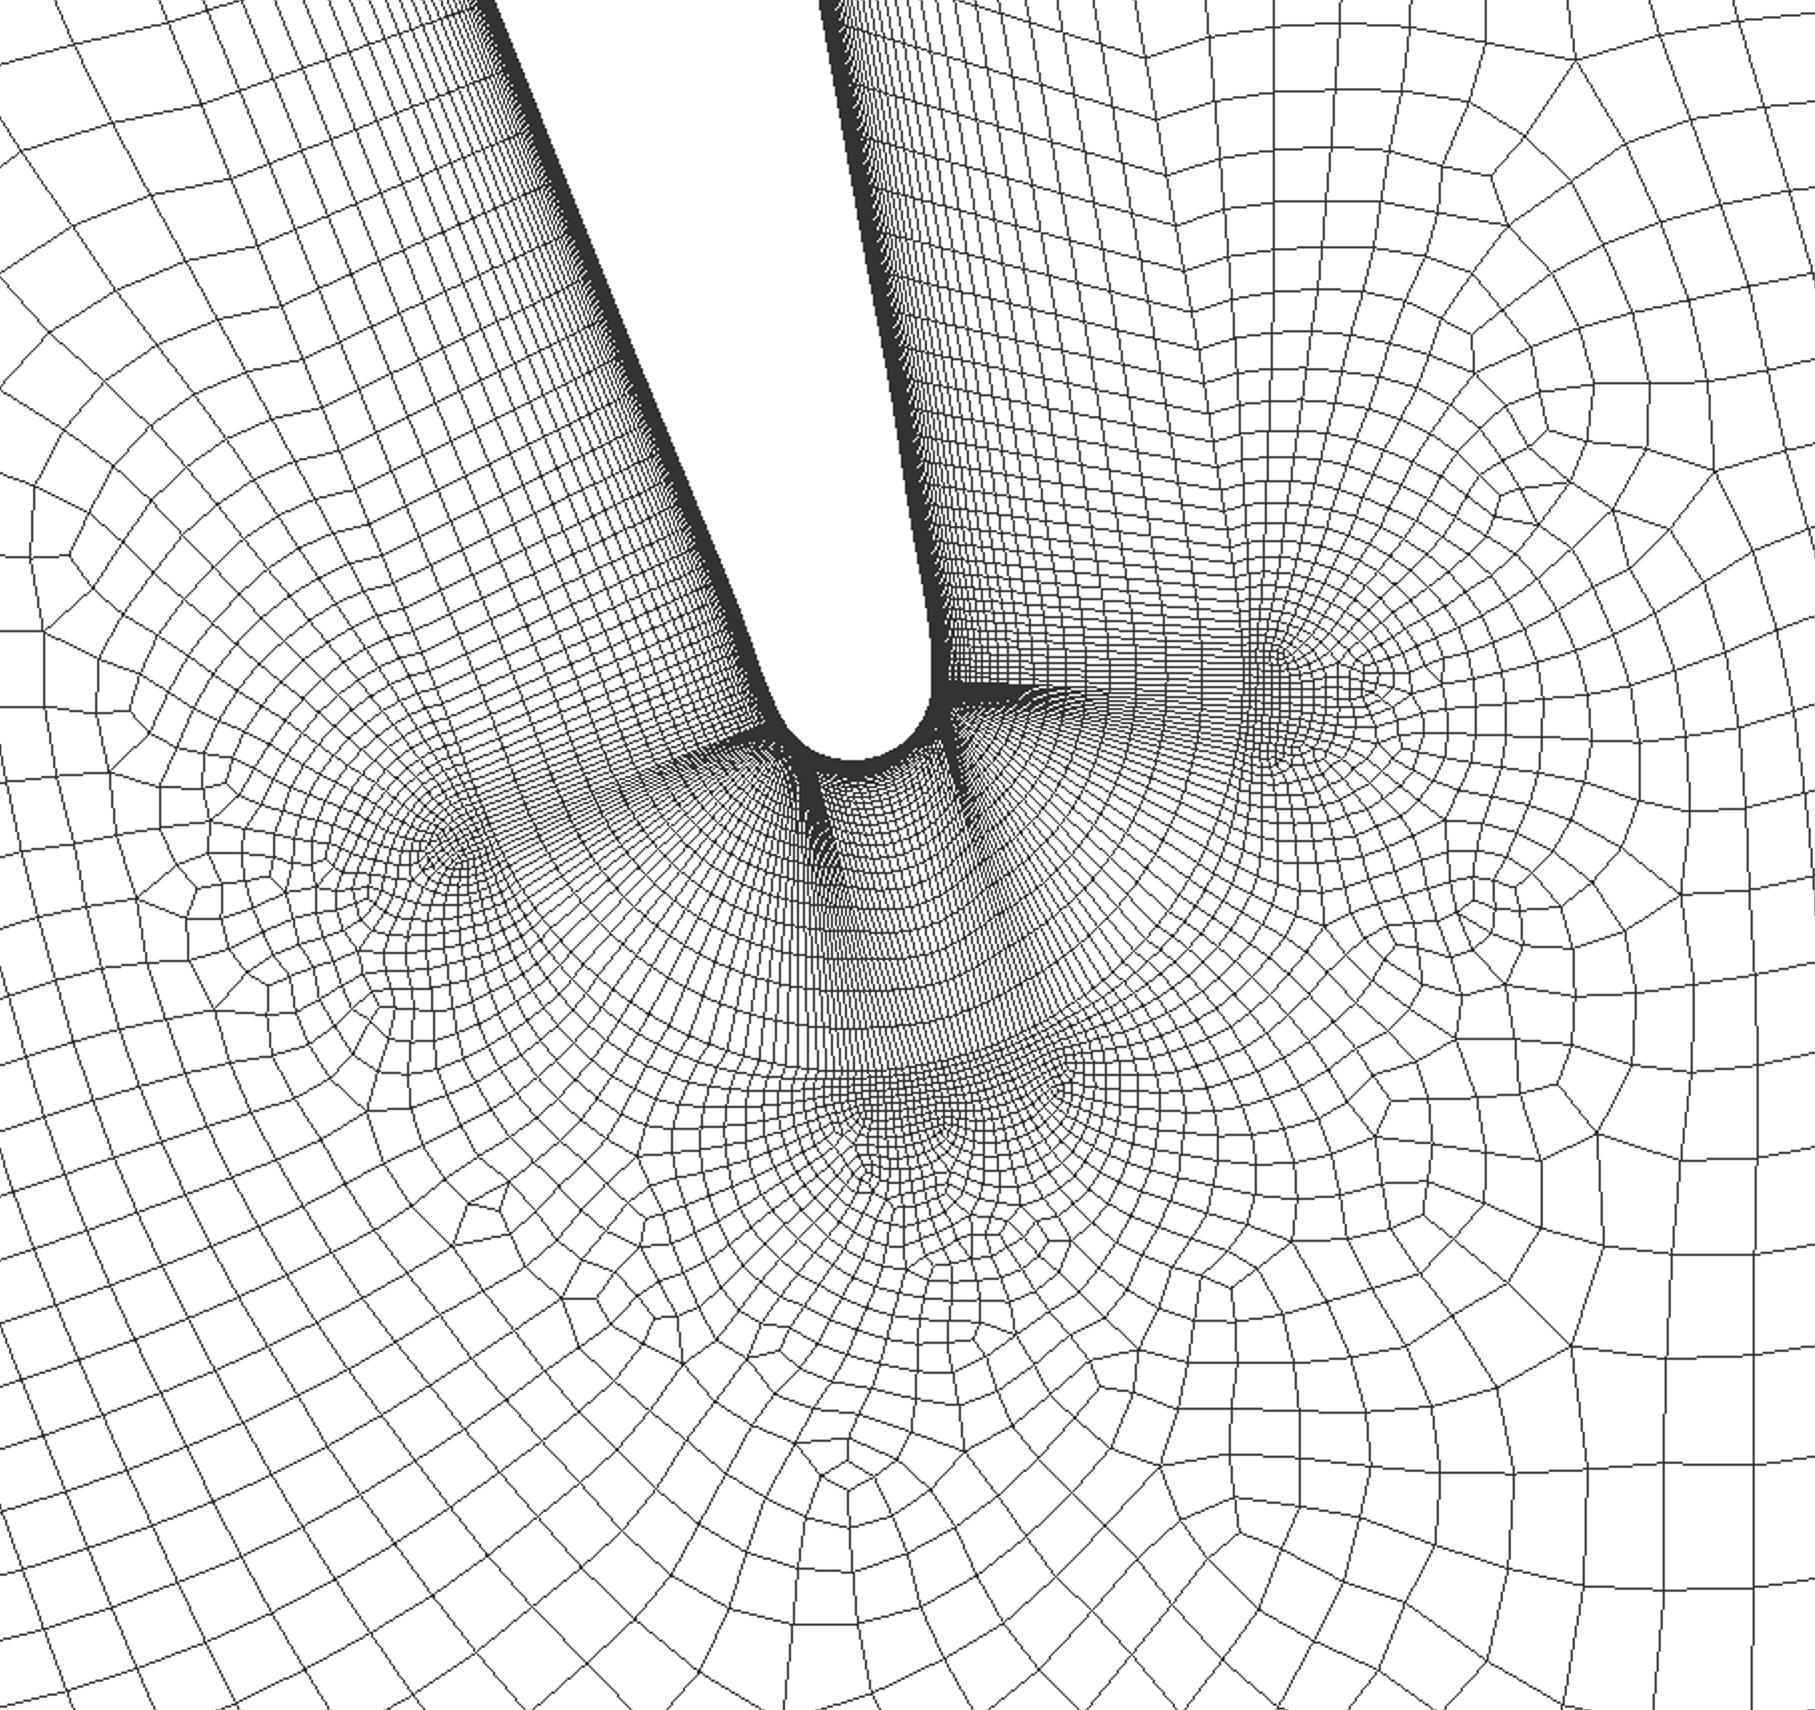
\includegraphics[width=\linewidth]{figs/t900_mesh_trailing_edge.png}
		\caption{Trailing edge}
		\label{fig:t900_mesh_trailing_edge}
	\end{subfigure}
	\caption{Details of mesh for Trent 900 throat width variation study}
	\label{fig:t900_mesh_details}
\end{figure}

The described mesh and boundary condition specifications were used to perform a series of CFD simulations of each of the 6 2D NGVs in Ansys Fluent 2020 R2. Solutions were initialised using the solver's built-in FMG initialisation. This procedure automatically constructs a coarser version of the supplied mesh, on which an initial solution is converged before refinement to the final resolution. More detailed explanation of the scheme is provided by Ansys~\cite{ansys_fmg_initialisation}. A script in the Fluent Journal language was used to produce solutions at incrementally increasing inverse pressure ratios of between $1.5$ and a fully choked inverse pressure ratio of $3.33$. NGV mass flow rate was saved at each pressure ratio. Full solution data were saved for the final fully choked pressure ratio to enable analysis of the shocks, expansions and sonic line at choked conditions. There were 32 increments of pressure ratio, and typical overall solution times were approximately 10 hours. The k-$\omega$ SST turbulence model was used. For these simulations and all others described in this thesis, convergence was determined by the outlet mass flow rate fluctuating by a factor of $10^{-6}$ or less. Mesh independence was verified by incrementally refining the mesh in Fluent and again confirming the outlet mass flow rate did not fluctuate significantly.

\subsection{Effect on 2D capacity}

Figure~\ref{fig:t900_mach_whole} shows contours of Mach number for one of the 6 solutions (vane KSZ03) at a fully choked pressure ratio. Streamlines released from the domain inlet illustrate the flow path through one of the vane passages. Figure~\ref{fig:t900_mach_throat} shown contours of Mach number for the same solution in the throat region.

\begin{figure}[H]
      \centering
      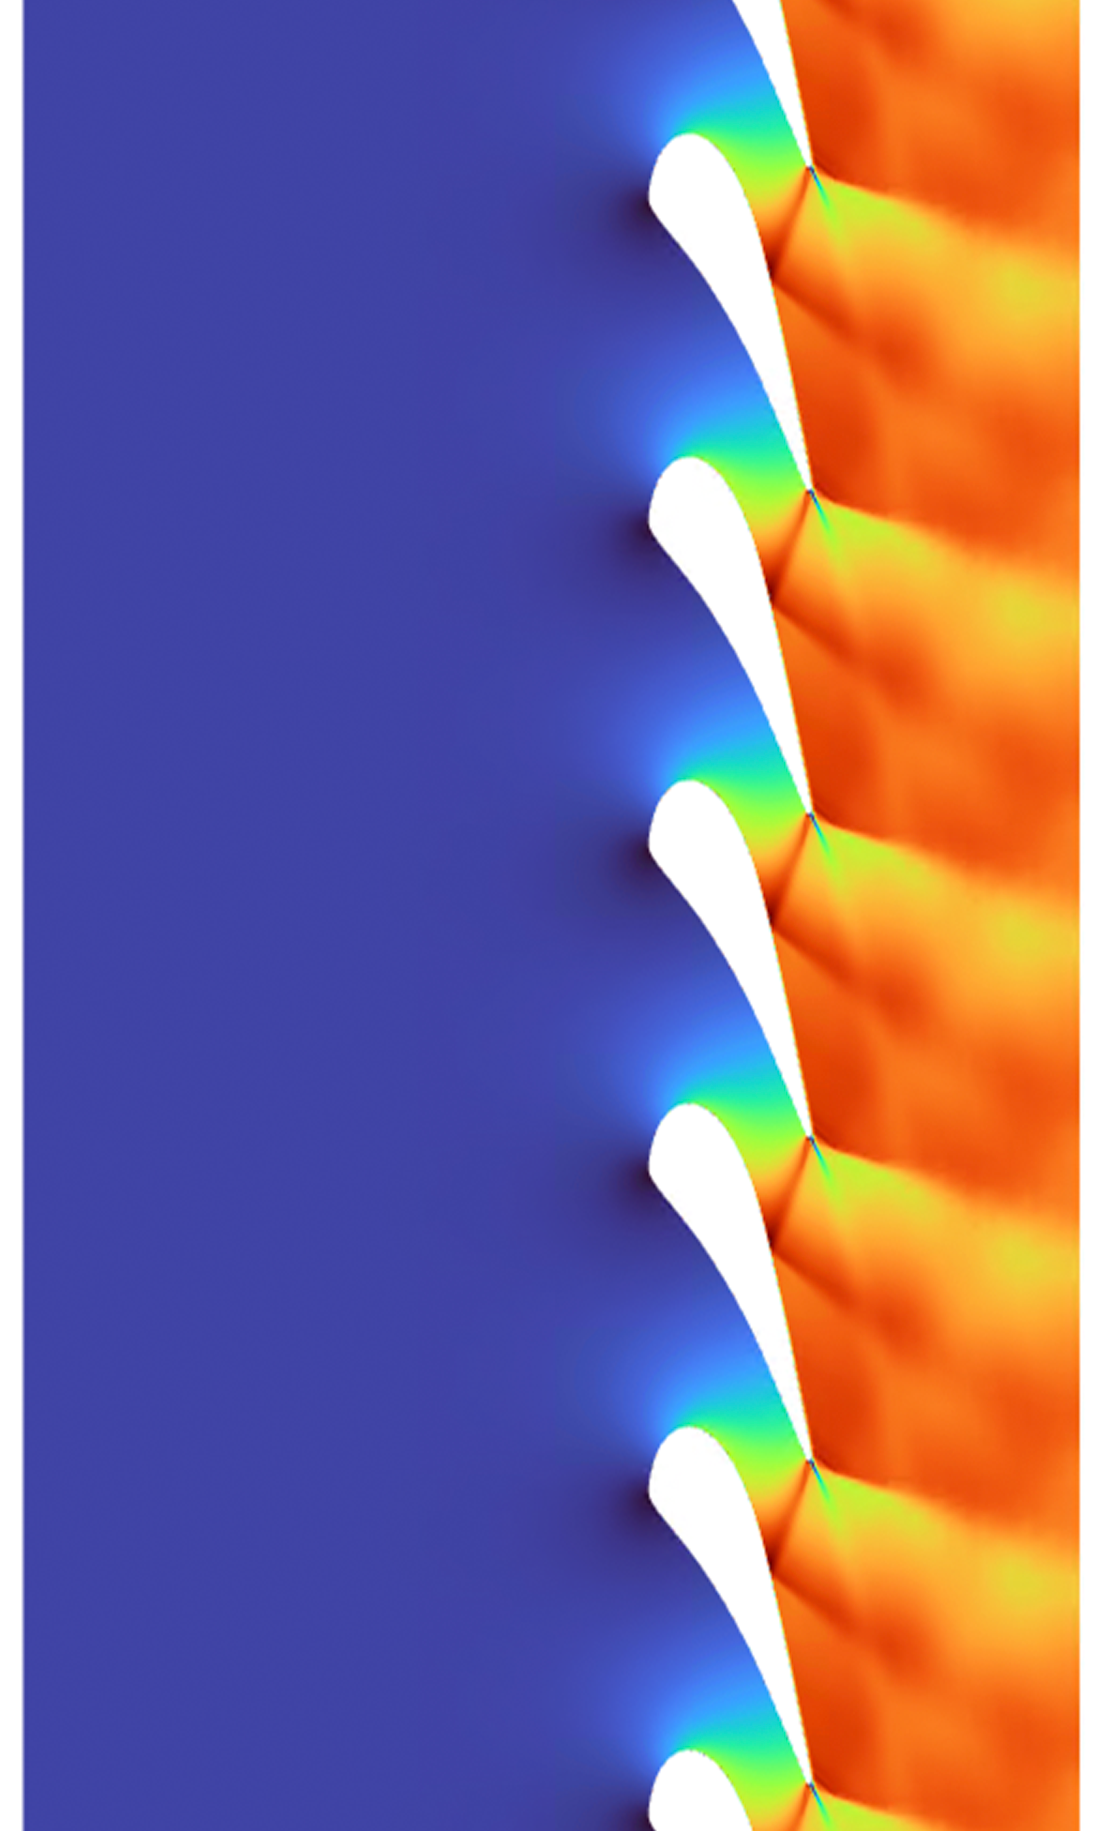
\includegraphics[width=.85\textwidth]{figs/t900_mach_whole.png}
      \caption{Contours of Mach number for whole solution on Trent 900 vane KSZ03 at $\frac{p_{01}}{p_2}=3.33$ with streamlines illustrating flow through a single vane passage}
      \label{fig:t900_mach_whole}
\end{figure}

\begin{figure}[H]
	\centering
	\begin{subfigure}{.15\textwidth}
		\centering
		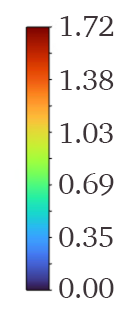
\includegraphics[width=\linewidth]{figs/mach_legend_choked.png}
	\end{subfigure}
	\hspace{0.05\textwidth}
	\begin{subfigure}{.45\textwidth}
		\centering
		
\includegraphics[width=\linewidth]{figs/t900_mach_throat.png}
	\end{subfigure}
	\caption{Contours of Mach number for solution near throat on Trent 900 vane KSZ03 at $\frac{p_{01}}{p_2}=3.33$}
	\label{fig:t900_mach_throat}
\end{figure}

Figures~\ref{fig:t900_mach_whole} and ~\ref{fig:t900_mach_throat} illustrate the presence of developed supersonic flow phenomena downstream of the throat. Expansion fans are observed as the flow expands through the region labelled A around the NGV trailing edge (which is not shaped this way in reality). Shockwaves are subsequently induced as the effective passage narrows due to the presence of the trailing edge wake. The pressure side shockwave reflects off the suction side of the adjacent NGV at the point labelled B, in a similar fashion to supersonic nozzle shock diamonds. These phenomena are in agreement with commonly seen flow features of NGVs in the supersonic regime. Figure~\ref{fig:t900_mach_throat} also illustrates the growth of a boundary layer on the downstream suction side of the NGV, labelled C. This boundary layer's interaction with the sonic line will be subsequently discussed in the context of its effect on flow capacity.

Figure~\ref{fig:t900_2d_capacity_trends} plots percentage changes in the flow capacity of the 6 NGVs (defined by equation~\ref{capacity_definition} and quantified by the upstream boundary conditions in Table~\ref{T900_parameters}) against inverse pressure ratio $\frac{p_{01}}{p2}$. Capacity changes are normalised against the capacity of vane KSZ03 at the design pressure ratio.

\begin{figure}[H]
	\centering
	$\Delta$ capacity $= \frac{\Gamma - \Gamma_{KSZ03}}{\Gamma_{KSZ03}}$
	\hspace{0.45cm}
	\begin{subfigure}{.45\textwidth}
		\centering
		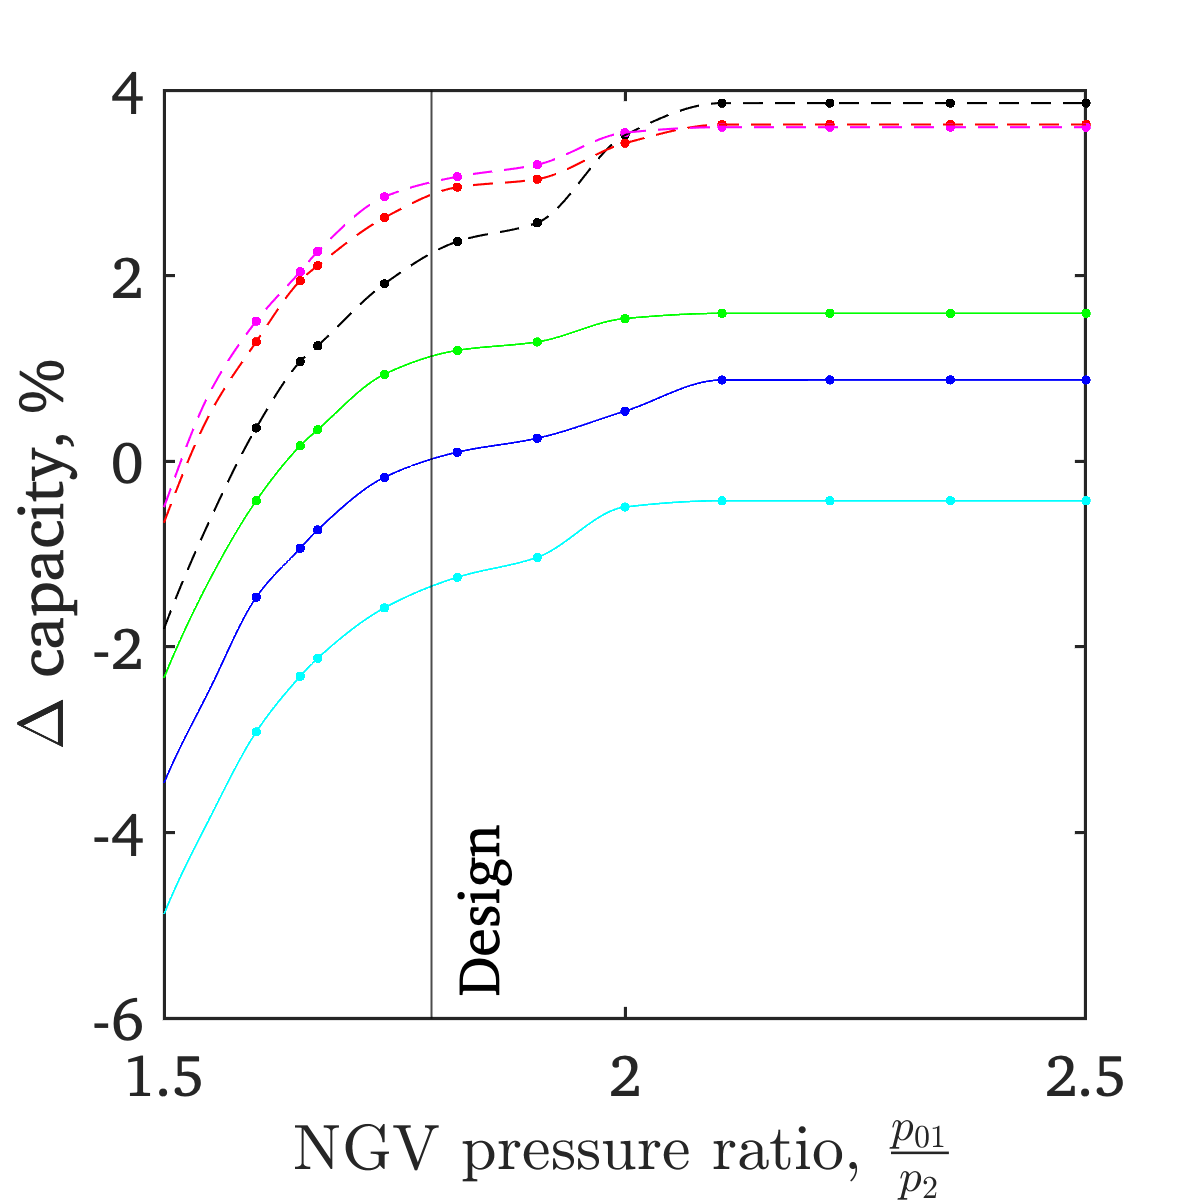
\includegraphics[width=\linewidth]{figs/t900_2d_capacity_trends.png}
	\end{subfigure}
	\begin{subfigure}{.1125\textwidth}
		\centering
		
\includegraphics[width=\linewidth]{figs/t900_2d_capacity_trends_legend.png}
	\end{subfigure}
	\caption{2D normalised capacity as a function of pressure ratio for 6 Trent 900 NGVs}
	\label{fig:t900_2d_capacity_trends}
\end{figure}

Differences are seen to exist between the capacity trends of the 6 NGVs. Across the range of pressure ratios, all 6 NGVs exhibited a range of approximately 4\% capacity difference. Although the NGVs were all fully choked at the greatest inverse pressure ratio, separate NGVs became choked at significantly different pressure ratios, suggesting that the formation of transonic flow features occurred in different locations between the 6 NGVs. The capacity trends are seen to be broadly divided between the M-skew family (K-- serial numbers) and the EP1 family (P-- serial numbers). The 3 M-skew NGVs had comparatively lower flow capacities than the EP1 NGVs at all pressure ratios. The capacities of the EP1 NGVs had comparatively small variation from one another across pressure ratios, but their homogeneity was broken by vane PNS04, which had the lowest flow capacity of the family at low inverse pressure ratio, but switched to have the highest flow capacity at high inverse pressure ratio.

The differing capacity trends may be further discussed by inspecting the shape of the sonic lines formed in the throat regions of the 6 NGVs at a fully choked pressure ratio. These sonic lines are depicted in Figure~\ref{fig:T900_mach1_lines} along with the lines of minimum length between the adjacent NGVs of each standard. 

\begin{figure}[H]
      \centering
      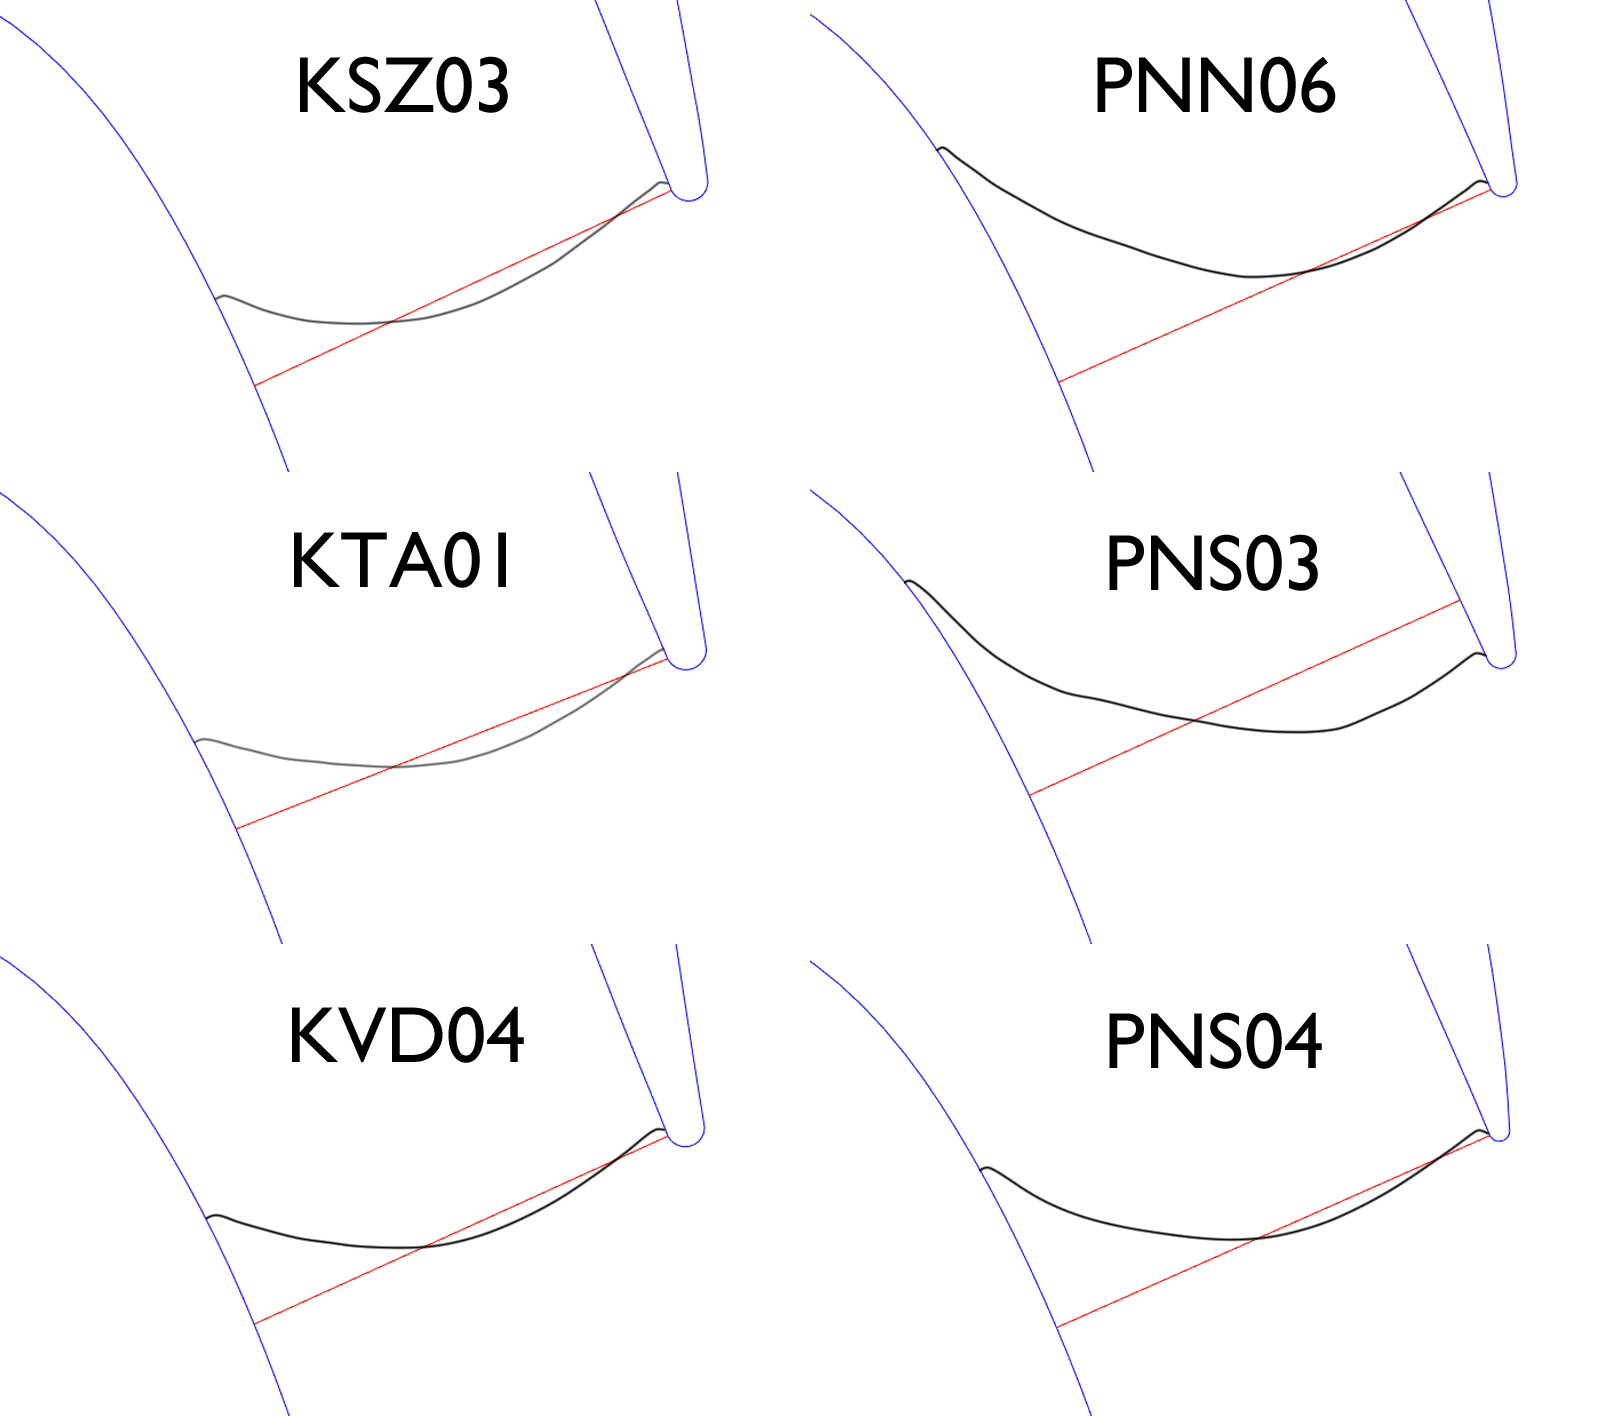
\includegraphics[width=.7\textwidth]{figs/T900_mach1_lines.png}
      \caption{Sonic lines for 6 Trent 900 NGVs at $\frac{p_{01}}{p_2}=3.33$}
      \label{fig:T900_mach1_lines}
\end{figure}

In Figure~\ref{fig:T900_mach1_lines}, a trend is visible of the M-skew sonic lines exhibiting smaller deviation from the line of minimum width, compared to the sonic lines of the EP1 NGVs. This suggests that a design choice resulted in a difference in the aerodynamics of the two families of NGV, such that upstream regions of the EP1 flow field reached sonic conditions significantly further upstream of the geometric throat compared to the M-skew flow field. Vane PNS04 presented a significantly different sonic line shape which is taken to correspond to its significantly different capacity trend compared to the other 2 vanes in its family. It is suggested that its relatively flow-orthogonal sonic line is caused by aerodynamic features that also cause its relatively sudden increase in capacity prior to choking. This cannot be confirmed in the absence of a statistically significant number of NGV geometries to compare.

Matlab was used to calculate the minimum throat width of each 2D NGV. The resulting values are given in Table~\ref{T900_throat_widths}.

\begin{table}[H]
\caption{Throat widths of 6 Trent 900 NGVs}
\label{T900_throat_widths}
\begin{center}
\begin{tabular}{|c|c|c|}
\hline
Production standard & Serial number & Throat width (mm)\\
\hline
\multirow{3}{*}{M EP1} & PNS04 & 12.7\\
 & PNN06 & 12.7\\
 & PNS03 & 12.7\\
\hline
\multirow{3}{*}{M-skew} & KTA01 & 12.5\\
 & KSZ03 & 12.4\\
 & KVD04 & 12.2\\
\hline
\end{tabular}
\end{center}
\end{table}

Discussion is warranted of the relationship between flow capacity and throat area. Consideration is to be made of both throat area in its pure geometric form $A$, and its effective from $A_{eff}$ as defined in equation~\ref{effective_throat_area_integral}. Figure~\ref{fig:T900_2d_capacities_vs_throat_widths} plots the 6 NGVs' variations in capacity at design pressure ratio against their variations in geometric throat width. Capacity changes are normalised against the capacity of vane KSZ03 at the design pressure ratio. Throat width changes are normalised against the geometric throat width of vane KSZ03. The averages of the M-skew and EP1 families are plotted and lines of gradient 1 are plotted intersecting the average values, such that any deviations from 1-dimensional compressible flow correspond to deviations from the lines of gradient 1.

\begin{figure}[H]
	\centering
	$\Delta$ capacity $= \frac{\Gamma - \Gamma_{KSZ03}}{\Gamma_{KSZ03}}$
	\hspace{0.45cm}
	\begin{subfigure}{.45\textwidth}
		\centering
		\includegraphics[width=\linewidth]{figs/T900_2d_capacities_vs_throat_widths.png}
	\end{subfigure}
	\begin{subfigure}{.1125\textwidth}
		\centering
		
\includegraphics[width=\linewidth]{figs/t900_throat_widths_legend.png}
	\end{subfigure}
	\caption{2D capacity percentage delta as a function of 2D throat width for 6 Trent 900 NGVs at $\frac{p_{01}}{p_2}=1.79$ (design)}
      \label{fig:T900_2d_capacities_vs_throat_widths}
\end{figure}

The 6 NGVs are seen to approximately conform to a directly proportional relationship between geometric throat width and flow capacity, suggesting that geometric throat width is a good estimator of flow capacity among NGVs without significant differences in aerodynamic design. The M-skew vanes exhibited notable conformity to this trend. This is in agreement with the observed homogeneity between the M-skew sonic line shapes. It it is suggested that, among the 3 vanes, the 2-dimensional sonic line shapes were scaling linearly with the shape of the geometric throat line, resulting in the observed linear relationship between geometric throat width and flow capacity despite the presence of a 2D flow field. 2D flow features appear to scale proportionately provided the sonic line scales proportionately.

In contrast, no correlation was observed between throat area and flow capacity among the EP1 NGVs. Speculation may be limited to the observation that the qualitatively distinct PNS04 vane exhibited significantly lower flow capacity than the other 2 despite having almost identical geometric throat areas. This highlights the difficulty in developing an a priori understanding of the observed capacity changes, even with knowledge of the NGV geometries as manufactured.

Although NGV throat width is a good predictor of NGV flow capacity if aerodynamics do not vary significantly, it is not useful if the sonic line is subject to unpredictable changes in shape and location. The resulting heuristic fails to account for the fact that the majority of streamlines within the flow reach sonic conditions at a point other than their point of minimum width. This discrepancy may be investigated by quantifying the effective throat width of each case, instead of the geometric throat area. Matlab was used to implement the integral
\begin{equation}\tag{\ref{effective_throat_area_integral}}
	A_{eff} = 
	\int_{1}^2 \vu*{u} \vdot \vu*{r} dL
\end{equation}

To achieve this, results for $M$ and $x$ and $y$ velocity components were exported from each Fluent solution. These data were imported into Matlab and interpolated onto a structured quadrilateral grid which covered the region around the throat between 2 adjacent NGVs. Within this domain, data points corresponding to the sonic line were identified using an algorithm to detect the cross-over from $M<1$ to $M>1$. A subsequent algorithm was used to order and connect these points into a sonic line. It was then possible to compute the local velocity unit vector $\vu*{u}$ and local unit vector orthogonal to the sonic line $\vu*{r}$ at each point, and to perform the integral. 

This resulted in Figure~\ref{fig:T900_2d_capacities_vs_effective_throat_widths}, which plots the 6 NGVs' variations in capacity at design pressure ratio against their variations in effective throat width. Capacity changes are normalised against the capacity of vane KSZ03 at the design pressure ratio. Effective throat width changes are normalised against the effective throat width of vane KSZ03. Because the concept of $A_{eff}$ is designed to account for generalised variations between NGVs, Figure~\ref{fig:T900_2d_capacities_vs_effective_throat_widths} does not group the NGVs into 2 separate families. A line of gradient $1$ is plotted and positioned on the $y$ axis to fit the data. It is notable that this line does not correspond to the line $y=x$, but instead corresponds to a negative offset in capacity. This suggests the presence of boundary layer effects which reduced the capacity compared to the values which effective throat area alone would predict.

\begin{figure}[H]
	\centering
	$\Delta$ capacity $= \frac{\Gamma - \Gamma_{KSZ03}}{\Gamma_{KSZ03}}$
	\hspace{0.45cm}
	\begin{subfigure}{.45\textwidth}
		\centering
		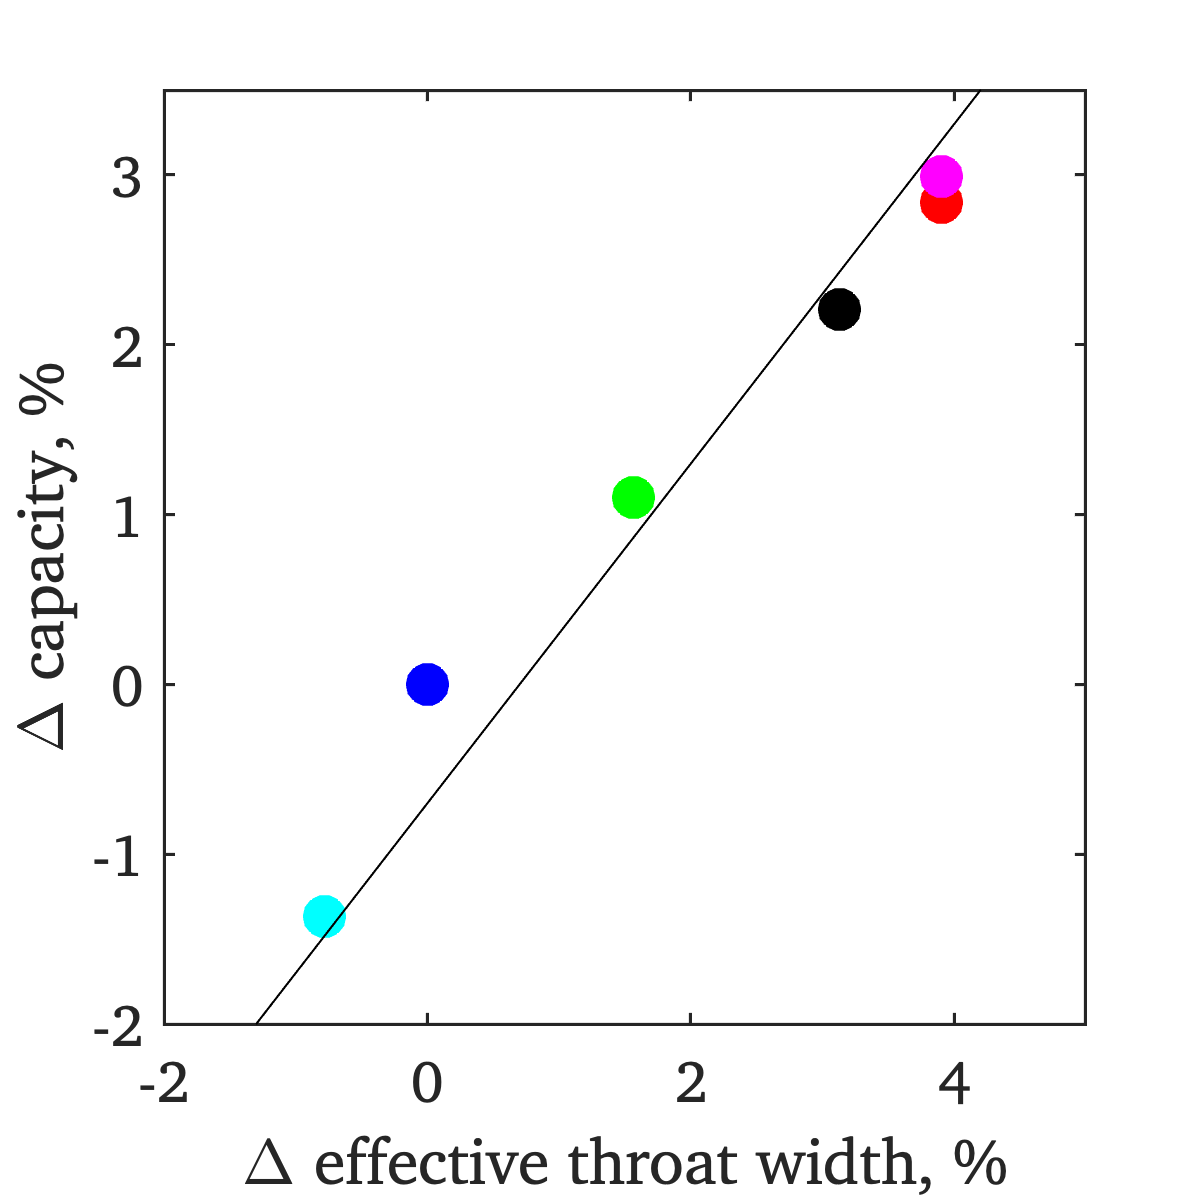
\includegraphics[width=\linewidth]{figs/t900_2d_capacities_vs_effective_throat_widths.png}
	\end{subfigure}
	\begin{subfigure}{.1125\textwidth}
		\centering
		
\includegraphics[width=\linewidth]{figs/t900_2d_capacity_trends_legend.png}
	\end{subfigure}
	\caption{2D capacity percentage delta as a function of effective throat width (as defined by equation~\ref{effective_throat_area_integral}) for 6 Trent 900 NGVs at $\frac{p_{01}}{p_2}=1.79$ (design)}
      \label{fig:T900_2d_capacities_vs_effective_throat_widths}
\end{figure}

Figure~\ref{fig:T900_2d_capacities_vs_effective_throat_widths} demonstrates the viability of the $A_{eff}$ approach. All six vanes approximately show a directly proportional relationship between flow capacity and effective throat width. This is in agreement with the assumption that the integral definition of $A_{eff}$ amounts to the summation of the 1-dimensional throat widths of every streamline in the flow. However, 3 of the NGVs exhibit significant deviation from direct proportionality, suggesting that the use of the sonic line fails to account for regions of the flow which remain subsonic given that the flow is largely unchoked. A possible refinement to the $A_{eff}$ approach may be to combine it with a prediction of the boundary layer thicknesses at the points where the sonic line meets the suction side and pressure side of the NGVs. Heuristics may be developed to relate the touch-down points with the predicted boundary layer thicknesses and thus the degree of $A_{eff}$ over-estimation caused by the inclusion of subsonic flow. This would result in a metric which is directly proportional to choked 2D capacity and closely correlated with 2D capacity at the design pressure ratio.

$A_{eff}$ remains computable only in the event that a CFD solution has been obtained, by which point flow capacity is already predicted. The next goal is to find an aspect of NGV geometry which can be shown to have a reliable effect on the shape of the sonic line. In this way, the geometric change will have been shown to account for a known change in $A_{eff}$, which has itself been shown to account for known changes in flow capacity in 2 dimensions. Since the M-skew and EP1 families exhibit clear differences in the sonic conditions which are present upstream of the geometric throat, future studies may examine whether NGVs can be reliably designed to have sonic lines whose shape is predictable. If the sonic line is known by design to be approximately orthogonal to the flow and non-susceptible to fluctuation, it is safe to rely on just 2D geometric throat width to predict variations in NGV flow capacity in 2 dimensions.


\section{Comparison of 2D capacity predictions with 3D data}
\label{2d_vs_3d_capacity_uncertainty}

The present study compared the 2D data presented in Section~\ref{section_1d_vs_2d_capacity_uncertainty} with Rolls-Royce's 3D CFD predictions of the flow capacities of the same 6 NGVs. The motivation was to analyse the differences between the 2D throat length vs capacity relationship and the 3D throat area vs capacity relationship. The analytical techniques of Section~\ref{section_1d_vs_2d_capacity_uncertainty} were translated to this 3D relationship where possible. As with the 2D study, the 3D vanes were uncooled, as were the vane platforms.

\subsection{Effect on 2D capacity versus 3D capacity}

Figure~\ref{fig:t900_3d_capacity_trends} plots percentage changes in the flow capacity of the 6 NGVs (defined by equation~\ref{capacity_definition} and quantified by the upstream boundary conditions in Table~\ref{T900_parameters}) against inverse pressure ratio $\frac{p_{01}}{p2}$. Capacity changes are normalised against the 3D capacity (as stated by Rolls-Royce) of vane KSZ03 at the design pressure ratio.

\begin{figure}[H]
	\centering
	$\Delta$ capacity $= \frac{\Gamma - \Gamma_{KSZ03}}{\Gamma_{KSZ03}}$
	\hspace{0.45cm}
	\begin{subfigure}{.45\textwidth}
		\centering
		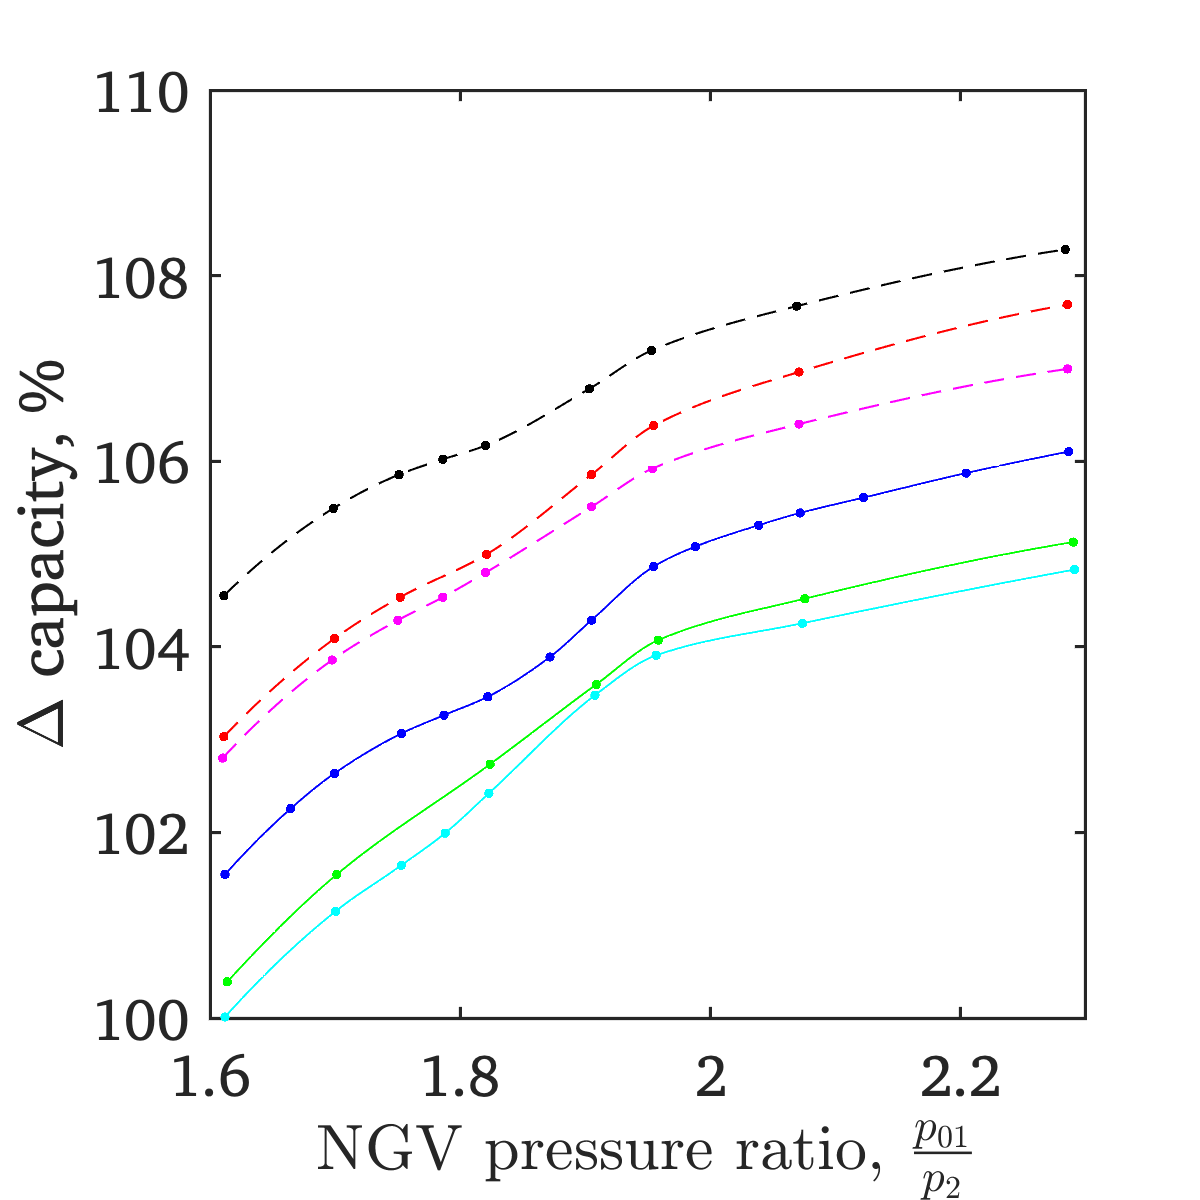
\includegraphics[width=\linewidth]{figs/t900_3d_capacity_trends.png}
	\end{subfigure}
	\begin{subfigure}{.1125\textwidth}
		\centering
		
\includegraphics[width=\linewidth]{figs/t900_2d_capacity_trends_legend.png}
	\end{subfigure}
	\caption{3D normalised capacity as a function of pressure ratio for 6 Trent 900 NGVs}
	\label{fig:t900_3d_capacity_trends}
\end{figure}

The predominant feature of Figure~\ref{fig:t900_3d_capacity_trends} is the continued rise in capacity with pressure ratio, in contrast to the 2D simulations where capacity plateaued between inverse pressure ratios of $2.0$ and $2.2$ for all $6$ NGVs. This suggests that none of the NGVs reached a fully choked condition over the entire range of pressure ratios. While regions of the NGV span must be choked at these higher inverse pressure ratios, a 3D NGV passage will exhibit secondary flow structures leading to progressive choking. A sufficiently high inverse pressure ratio will result in a flattening of the capacity trend as choking cannot progress further, but this limiting condition is not reached by the range of pressure ratios in the data provided by Rolls-Royce. This alone is sufficient to preclude the present $A_{eff}$ approach in these 3D cases, since it has been shown to be limited even by the presence of thin boundary layers in the 2D cases. In this case, a sonic surface may not exist as a flow-limiting condition, as there are unchoked alternative flow paths across the NGV span.

Zamboni~\cite{zamboni_area} defined the Rolls-Royce process for calculating 3D throat area as follows: ``Along each vane span section, the throat line is defined as that line which connects the trailing edge of one vane with the point of minimum distance on the suction surface of the nearby vane in the tangential direction. For a vane with a trailing edge slot, the trailing edge point is defined as the start of the cut back... The throat surface interpolates all the throat lines spanwise.'' It is notable that the engine maker has defined the geometric throat by assuming the trailing edge point to be the start of the cutback. Results in Chapter~\ref{chapter_trailing_edge} show this assumption to be inaccurate, as the 2D sonic line is observed to attach variously at this point or at the very end of the trailing edge, depending on precise cutback size.

The Rolls-Royce study produced values for throat area of the 6 NGVs in question. These values are listed in Table~\ref{T900_throat_areas}, where they are normalised against vane KSZ03 due to the sensitive nature of the data.

\begin{table}[H]
\caption{Throat areas of 6 Trent 900 NGVs}
\label{T900_throat_areas}
\begin{center}
\begin{tabular}{|c|c|c|}
\hline
Production standard & Serial number & $\Delta$ throat area, $\%$\\
\hline
\multirow{3}{*}{M EP1} & PNS04 & $1.2924$\\
 & PNN06 & $0.8616$\\
 & PNS03 & $0.5575$\\
 \hline
 \multirow{3}{*}{M-skew} & KTA01 & $0.3928$\\
 & KSZ03 & $0.0000$\\
 & KVD04 & $-0.4435$\\
\hline
\end{tabular}
\end{center}
\end{table}

The viability of the geometric throat area approach to 3D data is illustrated in Figure~\ref{fig:T900_2d_capacities_vs_throat_areas}, which plots the 6 NGVs' variations in capacity at design pressure ratio against their variations in geometric throat area. Capacity changes are normalised against the 3D capacity (as stated by Rolls-Royce) of vane KSZ03 at the design pressure ratio. Throat area changes are normalised against the 3D throat area (as stated by Rolls-Royce) of vane KSZ03. The averages of the M-skew and EP1 families are plotted and lines of gradient 1 are plotted intersecting the average values, such that any deviations from 1-dimensional compressible flow correspond to deviations from the lines of gradient 1.

\begin{figure}[H]
	\centering
	$\Delta$ capacity $= \frac{\Gamma - \Gamma_{KSZ03}}{\Gamma_{KSZ03}}$
	\hspace{0.45cm}
	\begin{subfigure}{.45\textwidth}
		\centering
		\includegraphics[width=\linewidth]{figs/T900_3d_capacities_vs_throat_areas.png}
	\end{subfigure}
	\begin{subfigure}{.1125\textwidth}
		\centering
		
\includegraphics[width=\linewidth]{figs/t900_throat_widths_legend.png}
	\end{subfigure}
	\caption{3D capacity percentage delta as a function of 3D throat area for 6 Trent 900 NGVs at $\frac{p_{01}}{p_2}=1.79$ (design)}
      \label{fig:T900_2d_capacities_vs_throat_areas}
\end{figure}

Figure~\ref{fig:T900_2d_capacities_vs_throat_areas} shows that no correlation exists between geometric throat area and flow capacity for the 6 NGVs simulated by Rolls-Royce. This is in agreement with the hypothesis that highly 3-dimensional flow phenomena are present to a degree that predominates over any area-capacity relationship. Future study might divide focus between developing a 3D version of the $A_{eff}$ technique and accessorising it with a model for the subsonic secondary flows that are hypothesised to be present even at the fully choked pressure ratio used to evaluate $A_{eff}$ in the 2D cases. An overarching goal may be to confirm that secondary flows are indeed the confounding factor that is not captured by 2-dimensional CFD. In any case, motivation is presented to resolve the failure of present analytical techniques in understanding the sensitivity of nozzle guide vane flow capacity to geometric changes.

\section{Chapter conclusions}

Variations in the cast shape of nozzle guide vanes have been shown to cause variations in their predicted flow capacity. 2D CFD simulations have been performed on a family of 6 NGVs which were selected by Rolls-Royce to be representative of random variations in the shape of Trent 900 engine parts after they have been cast but before cooling features have been machined in. 

At the NGVs' design inverse pressure ratio, the design flow capacity of the 6 vanes has been found to correlate to some extent with both the vanes' geometric throat area and with the effective throat width $A_{eff}$. 2D geometric throat width can be evaluated from the NGV design geometry without any further computational effort, but $A_{eff}$ cannot be evaluated without obtaining a CFD solution at a fully choked pressure ratio. The $A_{eff}$ approach is thus offered not as a means to predict the flow capacity of a given geometry, but rather as a means to quantify the shape of the 2-dimensional sonic line that forms at a fully choked pressure ratio, and to discuss this shape's effect on capacity.

Nozzle guide vane flow capacity correlates well with $A_{eff}$ at the design pressure ratio despite the non-existence of a sonic line when the flow is not fully choked. This suggests that the sonic line shape is driven by the same geometric factors that drive the 2-dimensional flow field prior to choking. Thus for a given NGV production standard that outputs sets of vanes with casting variations, two conclusions can be drawn from simulating a representative sample of the vanes in 2D. Firstly any scanned vane's 2D capacity will be well-predicted by its 2D throat width if fully choked simulations have shown the sonic line to exhibit relatively small deviation from the geometric throat line. Secondly the whole production standard is likely to have reduced capacity predictability if fully choked simulations have shown the sonic line to vary significantly in shape between individual vanes.

Conclusions are more difficult to draw in the case of 3D capacity, where a 3D extension of the $A_{eff}$ approach is rational but would require careful adjustment for the delayed onset of choking in 3D compared to 2D. Where Section~\ref{section_1d_vs_2d_capacity_uncertainty} suggested a boundary-layer model as a future addition to the technique, Section~\ref{2d_vs_3d_capacity_uncertainty} has presented data from 3D geometries for which the equivalent inverse pressure ratio of $3.33$ would produce significant regions of secondary flow which are not choked. These regions may be accounted for by an appropriate model or negated by the use of an even higher inverse pressure ratio. The overall conclusion of this chapter is that future analyses of casting variations versus flow capacity should involve 3D simulation, should account for both boundary layers and secondary flows when conceptualising $A_{eff}$ in 3D, and should use a statistically significant number of scanned vanes to produce two key metrics. Firstly the mean departure of the vanes' sonic surfaces from the surface of minimum area will reveal whether the minimum area is a useful capacity predictor for that production standard. Secondly the variance of the vanes' sonic line shapes will indicate that production standard's capacity uncertainty.


\chapter{Trailing edge shape}
\label{chapter_trailing_edge}
%How the trailing edge can drive capacity changes (and loss changes incidentally). These changes are discussed as those happening in-life to the existing engine parts, and also those resulting from an alternative design.
%Why am I including "loss" here, when this part is really about the robustness of capacity predictions on vanes that will change shape with wear? Because the proposed alternative design needs to be decent for loss to be a viable alternative.

%NEEDED DATA:
%-SS cutbacks, all solutions
%-PS cutbacks, all solutions
%-variable cooling rate CFD
%-Larger pictures of the different meshes used
%-Larger contour plots for the different levels of TE SS erosion
%-MinA and M1 lines for the TE SS cutbacks  
%-"Rolls-Royce vs this study" geometry illustration should be remade to be at the same angle as all the flow pictures

%Plan for chapter - answer the following questions:
%1) How does erosion to the SS end-edge alter 2D mid-span capacity, and which mechanism best explains the changes?
%2) According to the literature, would a 3D investigation into this be justified?
%3) How capacity-predicable would an altrernative design of TE be?
%4) Would said alternative design reduce "loss"?

Nozzle guide vane flow capacity is known to be a function of effective throat area. Thus we must survey the practical reasons for which effective throat area might vary. In a real engine, NGV effective throat area may depart from its design value if the NGVs depart from the ideal aerodynamic design shape. This may occur through practical design choices for reasons such as cooling or blockage avoidance, because of the finite precision of manufacturing, or because of erosion while in service. 

A goal of the present study is to help ascertain how much such design decisions and off-design conditions affect the predictability of NGV flow capacity, and to comment on ways to mitigate this limitation. The NGV trailing edge is an area of focus because it is particularly susceptible to both finite-precision and in-service departures from its design shape. It is also difficult to model small features accurately using CFD, so knowledge of which features may be neglected will enable faster and more extensive design calculations.

The trailing edge is susceptible to finite-precision departures from its design shape because of how it is manufactured. Vane pairs are cast to a finite precision as discussed in Section~\ref{section_1d_vs_2d_capacity_uncertainty}, where significant geometric variation appears even prior to the addition of cooling features. The vanes are then machined to finish off the trailing edge shape to a high tolerance. The finishing creates the aerodynamically best possible trailing edge. 

The trailing edge's principal design feature is the difference between the amount of material left on the suction side of the coolant ejection slot and the amount left on the pressure side. This creates the thinnest possible final trailing edge for the vane with the intent of minimising separated wake area and thus loss. The resulting feature will be referred to as the end-edge in this thesis, and is illustrated in Figure~\ref{fig:te_features_labelled}. The end-edge depends on the slot coolant flow for protection against in-service erosion. The ideal coolant ejection slot width may be determined as the width through which the coolant would be ejected between it and the mainstream flow.

\begin{figure}[H]
      \centering
      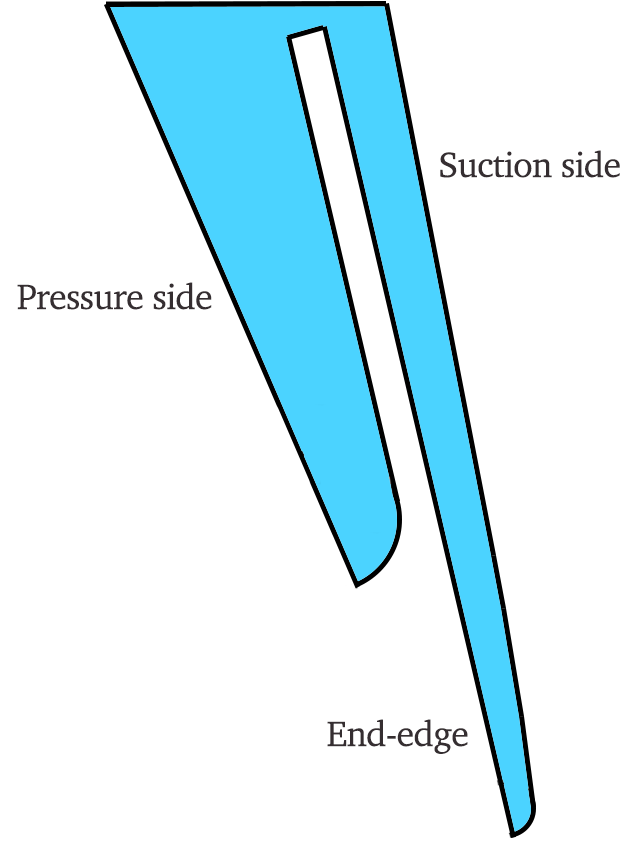
\includegraphics[width=.45\textwidth]{figs/te_features_labelled.png}
      \caption{Main features of a contemporary nozzle guide vane trailing edge}
      \label{fig:te_features_labelled}
\end{figure}

The 3-dimensional design of contemporary nozzle guide vanes assumes they will be cast in pairs of vanes together with their inner and outer annulus end-walls.They feature a filleted transition to allow the end-edge to cleanly meet the end-walls, and an end-edge chord length that is consistent across its span. The creation of a repeatable minimum geometric area which provides the required turning and flow capacity is a primary objective, but so is generating a vane with minimal loss at the start of its service life. These design goals are not necessarily aligned, and it may be the case that  a loss-optimised NGV trailing edge is suboptimal in terms of the design's repeatability or susceptibility to unintended changes while in service.

The trailing edge is the part of the vane most susceptible to in-service departures from its build design because it is vulnerable to both cooling and aerodynamic damage. The NGV remains largely intact over its lifetime despite the external gas temperature and high speed external flow. In contrast, the end-edge is subject to significant erosion. If there is a blockage in any of the plena which feed the trailing edge slot, part of its span will receive reduced coolant flow, accelerating the oxidation degradation of the end-edge in that region. Such cooling failures are not uncommon in sandy environments. In such environments, film cooling holes on the pressure side are particularly vulnerable to damage, and this has lead to the adoption of the ``cut-back'' trailing edge, where the trailing edge region is protected by coolant from the trailing edge slot that is shielded from the mainstream flow to prevent blockage. The pay-off is that the end-edge is now cooled by an external film which must remain attached and is subject to entrainment from the mainstream flow.

The nozzle guide vane must provide a repeatable setting for engine core flow capacity, correct flow turning, and minimal loss. This chapter will predict and analyse these metrics for cases where the shape of the trailing edge is subject to variation. Variations will include incremental reduction in the end-edge length associated with in-service erosion, and incremental reduction in the pressure-side cut-back length as a design variable. The first section of this chapter will review the literature on various definitions of loss, which provides a key measure of performance.


\section{Definitions of loss for trailing edge performance evaluation}
\label{definitions_of_loss}
%--How does it perform in terms of loss?
%--First review the literature to decide what is "loss".

Loss may refer to any process whereby the recoverable energy of a turbomachinery flow is reduced during transit through a turbine stage, other than by shaft work, with corresponding entropy creation. Minimisation of loss remains a primary objective of turbomachinery design, but there is not a universal consensus on how to quantify it. As subsequent sections of this thesis will evaluate the losses caused by changes to the trailing edge of nozzle guide vanes, the purpose of this section is to review various definitions of loss from the literature and to facilitate the use of appropriate definitions in the present study.

Trinidade et al~\cite{trinidade_loss} characterised sources of loss as shock loss, profile losses, tip leakage, end-wall losses, and cooling losses. Tip leakage results from flow through the clearance space between blade tips and their annular casing. It will not be considered by the present study, since in the present study NGVs are cast along with their end-walls. End-wall losses result from 3-dimensional secondary flows, and will not be considered in the present study which is of 2-dimensional phenomena.

Trinidade et al~\cite{trinidade_loss} characterised shock loss as resulting from entropy creation across the shock wave during supersonic flow. The present study will consider this mechanism during discussion of CFD results at choking pressure ratios.

Profile loss was characterised by entropy creation by viscosity in the boundary layer on the blade surface. Entropy generated near the blade's trailing edge was considered as profile loss due to the high entropy creation in the wake region following flow separation at the trailing edge. The authors extended this definition to include the entropy generated as the flow turns tightly around the trailing edge curvature and forms expansion waves.

The authors also defined the category of cooling losses to refer to the aerodynamic penalties incurred by cooling in general, namely ``thicker blade profiles from coolant holes, interaction of coolant film with the blade boundary layer, mixing losses between coolant and main flow and endwall losses.'' The present study seeks to isolate the mechanisms whereby film cooling causes boundary layer changes and mixing effects, discussing film cooling in Chapter~\ref{chapter_leading_edge}.

The present study seeks to define a coefficient of NGV total pressure loss whose arguments are flow measurements or numerically predicted parameters. It is first useful to consider the motivation for quantifying loss in terms of total pressure. This approach treats the nozzle guide vane problem analogously to the problem of flow in a rough pipe, where frictional forces must be balanced by a negative total pressure gradient in the downstream direction. The greater the sum of frictional forces, the greater the loss of total pressure between the inlet and outlet. Total pressure loss can thus aggregate all aerodynamic drag forces acting on the nozzle guide vane or other component.

In an experimental or computational domain, the total pressure loss between inlet and outlet is $p_{01} - p_{02}$. It is intuitive to normalise this against the upstream total pressure $p_{01}$ but it is more useful to normalise it against $p_{01} - p_2$, where $p_2$ is the outlet static pressure. $p_{02}$ never assumes a value greater than $p_{01}$ nor less than $p_2$, so if a total pressure loss coefficient is quantified as
\begin{equation}\label{total_pressure_loss_coefficient}
C_{pt} = \frac{
p_{01} - p_{02}
}{
p_{01} - p_2
}
\end{equation}
then the coefficient will be $0$ in the case of no total pressure loss, and $1$ in the extreme case of $p_{02} = p_2$.

Giel et al~\cite{giel_te_thickness}, whose findings will be discussed in Section~\ref{performance_of_an_alternative_trailing_edge_design}, surveyed the total pressure wake profiles of a blade at mid-span. They defined a total pressure loss coefficient as in equation~\ref{total_pressure_loss_coefficient}, where $p_{01}$ and $p_{02}$ were the inlet and wake total pressures, and $p_2$ was the wake static pressure. 

Gao et al~\cite{gao_te}, whose findings will be discussed in section~\ref{suction_side_cutbacks}, defined a total pressure loss coefficient as
\begin{equation}
C_{Gao} = \frac{
p_{01} - p_{02}
}{
p_{02} - p_2
}
\end{equation}

This definition is equivalent to normalising the total pressure loss against the downstream dynamic pressure. In the case of simulations where the boundary conditions $p_{01}$ and $p_2$ are set, NGV geometry is the independent variable and $p_{02}$ is the dependent variable. It is thus less convenient for the present study to use Gao et al's~\cite{gao_te} loss coefficient formulation, since it does not scale linearly across a range of $p_{02}$. The definition in equation~\ref{total_pressure_loss_coefficient} will be used for this reason.

Where subsequent sections are to compare the findings of Giel et al~\cite{giel_te_thickness}, Gao et al~\cite{gao_te}, and other studies of loss, it is required to formulate the total pressure loss coefficient consistently. Gao's~\cite{gao_te} definition of $C_{pt}$ may be expanded by Taylor series on the constant $p_{01}$ and as a function of $p_{02}$ as
\begin{equation}
f\left(p_{02}\right) = \\
f\left(p_{01}\right) +
f'\left(p_{01}\right) \left(p_{02} - p_{01}\right) +
\frac{1}{2!} f''\left(p_{01}\right) \left(p_{02} - p_{01}\right)^2 +
...
\end{equation}
where $f^n\left(p_{01}\right)$ may be shown by differentiation to be
\begin{equation}
f^n\left(p_{01}\right) =
\frac{
	\left(-1\right)^n n !
}{
	(p_{01} - p_2)^n
}
\end{equation}
This results in the following mappings between the two definitions of total pressure loss coefficient.
\begin{equation}
C_{Gao} = 
\sum_{n=1}^{\infty}
C_{pt}^n
\end{equation}
\begin{equation}
C_{pt} = 
\sum_{n=1}^{\infty}
\left(-1\right)^{n-1}
C_{Gao}^n
\end{equation}

Since the total pressure loss coefficient quantifies loss as a summation of all drag forces on the NGV, loss may also be quantified as the total amount of kinetic energy dissipated between inlet and outlet, of the form
\begin{equation}\label{ke_loss_form}
\zeta =
\frac{KE_1 - KE_2}{KE_1}
=
1 - \frac{KE_2}{KE_1}
\end{equation}

Kinetic energy may be formulated using conservation of energy as
\begin{equation}\tag{\ref{compressible_bernouilli}}
u = 
\sqrt[•]{ 
2 \left( \frac{\gamma}{\gamma - 1} \right) \left[ \frac{p_0}{\rho_0} - \frac{p}{\rho} \right] 
}
\end{equation}
\begin{equation}
u =
\sqrt[•]{ 
	2 \left( \frac{\gamma}{\gamma - 1} \right)
	R T_0
	\left[
		1 - \left(
			\frac{p_0}{p}
		\right)
		^\frac{1-\gamma}{\gamma}
	\right] 
}
\end{equation}
The flow's kinetic energy at a given station is thus of the form
\begin{equation}
KE(p) 
\sim
u^2
\sim
1 - \left(
	\frac{p_0}{p}
\right)
^\frac{1-\gamma}{\gamma}
\end{equation}
allowing equation~\ref{ke_loss_form} to be written as
\begin{equation}
\zeta = 
1 - 
\frac{
	1 -
	\left(
		\frac{p_{02}}{p_2}
	\right)
	^\frac{1-\gamma}{\gamma}
}{
	1 -
	\left(
		\frac{p_{01}}{p_2}
	\right)
	^\frac{1-\gamma}{\gamma}
}
\end{equation}
\begin{equation}\label{ke_loss_definition}
\zeta = 
\frac{ 
	\left(
		\frac{p_{01}}{p_{02}}
	\right)
	^\frac{\gamma-1}{ \gamma } - 1 
}{
	\left(
	\frac{p_{01}}{p_{2}}
	\right)
	^\frac{\gamma-1}{ \gamma } - 1 
}
\end{equation}
This definition of kinetic energy loss coefficient was used by Giel et al~\cite{giel_te_thickness}. Like the total pressure loss coefficient, it takes a value of $0$ in the case of no loss where $p_{02} = p_{01}$, and $1$ in the extreme case of $p_{02} = p_2$.

Saha et al~\cite{saha_loss} experimentally investigated the loss effects of shower-head and trailing edge cooling in an annular sector. By defining kinetic energy loss in 3 alternative ways, the authors demonstrated the extent to which computed loss can vary depending on definition. Discrepancies were shown to result from how the coolant kinetic energy is accounted for. Where the ratio of coolant mass flow rate to mainstream mass flow rate was $Y$, the authors defined kinetic energy loss as
\begin{equation}\label{saha_loss_definition}
\zeta = 
1 -
\frac{ 
	\left( 1 + Y \right) 
	\left[
		1 -
		\left(
			\frac{p_2}{p_{02}}
		\right)
		^\frac{\gamma-1}{\gamma}
	\right]
}{
	\left[
		1 -
		\left(
			\frac{p_2}{p_{01}}
		\right)
		^\frac{\gamma-1}{\gamma}
	\right]
	+Y
	\left[
		1 -
		\left(
			\frac{p_2}{p_{0c}}
		\right)
		^\frac{\gamma-1}{\gamma}
	\right]
}
\end{equation}
In the case of no coolant flow ($Y=0$) this is equivalent to the definition in equation~\ref{ke_loss_definition}. Equation~\ref{saha_loss_definition} is equivalent to the loss definition defined by Deckers and Denton~\cite{deckers_loss} in the case of no significant temperature difference between coolant and mainstream, as in a significant proportion of experimental studies.

Where coolant flow is present, equation~\ref{saha_loss_definition} requires a local value of $Y$ in order to obtain the loss at any particular point. Assuming that the coolant concentration is a function of the local total pressure loss compared to an uncooled vane, the authors redefined $Y$ as a function of spanwise distance $x$ as
\begin{equation}
\frac{Y\left(x\right)}{Y_{max}}
=
\frac{
	p_{02uc} - p_{02}\left(x\right)
}{
	\left| p_{02uc} - p_{02} \right|_{max}
}
\end{equation}
where $p_{02uc}$ was the total pressure downstream of the cascade with no cooling, $p_{02}$ was the total pressure downstream of the cascade as a function of spanwise distance (with cooling), and $\left| p_{02uc} - p_{02} \right|_{max}$ denotes the maximum possible difference in downstream total pressure between the uncooled and the cooled cases. Reasoning that this total pressure difference is maximal when $p_{02}=p_{01}$ and $p_{02}=p_{wake}$ (the total pressure in the wake region), Saha et al~\cite{saha_loss} thus defined their function for local coolant/mainstream mass flux ratio as
\begin{equation}
\frac{Y\left(x\right)}{Y}
=
\frac{
	p_{02uc} - p_{02}\left(x\right)
}{
	p_1 - p_{02wake}
}
\end{equation}
By substituting this definition of $Y$ into equation~\ref{saha_loss_definition}, Saha et al~\cite{saha_loss} arrived at their novel definition of kinetic energy loss intended to solve the problem of unphysical loss in the free-stream where the previous definition erroneously assumed the presence of coolant. Their new definition is able to use the nominal values for shower-head and trailing edge coolant mass flow ratio and adjust the coolant profile according to the aforementioned function of spanwise distance. Using measurements from a downstream traverse in their linear cascade, the novel loss definition was found to produce loss profiles that were in good agreement with equation~\ref{ke_loss_definition} and in disagreement with equation~\ref{saha_loss_definition}.


\section{Effects of suction-side trailing edge shape uncertainty}
\label{suction_side_cutbacks}

The end-edge, which forms the sharp tip of the trailing edge, is formed from material on the suction side of the NGV passage. This section will consider increasingly severe loss of material up to a potential worst case for in-service erosion of the end-edge, namely its complete deletion. Erosion has been assumed to take place at the NGV mid-span where flow speeds and temperatures are highest and there is previous anecdotal evidence of in-service damage. Here secondary flows across the blade are small and a 2-dimensional simulation of the mid-span flow should provide a physically realistic measure of performance.

\subsection{Geometry, mesh, and boundary conditions}

2D CFD has been used to model the effects of incremental removal of material from the suction-side end-edge of an NGV. The baseline geometry is vane KSZ03 from the 6 vanes provided by Rolls-Royce for the work discussed in Chapter~\ref{chapter_geometric_throat_area}. The 2D vane section was produced using the process illustrated in Figure~\ref{fig:2d_geometry_creation}. The overall computational domain was produced as in Figure~\ref{fig:computational_domain_and_boundaries}. Unlike the section of vane KSZ03 studied in Chapter~\ref{chapter_geometric_throat_area}, the NGV trailing edge was not rounded but realistically shaped based on GOM scan analysis, and the domain was modified to include a flow inlet within the NGV's trailing edge slot, where the mass flow rate to be ejected was specified. The boundary conditions used for all simulations are as listed in Table~\ref{ss_cutbacks_parameters}.

Simulations were performed at a range of inverse pressure ratios between $1.5$ and $3.33$, and particular study was made at inverse pressure ratios of $1.5$, $1.79$ and $3.33$. This permits comment on the NGV flow capacity as a function of only the sonic line shape, and eliminates the possibility of unchoked flow passing through the nozzle, with the exception of the boundary layers. $\frac{p_{01}}{p_2}=3.33$ was considered to be a case where the nozzle guide vane is definitely fully choked. Although this particularly high inverse pressure ratio is possibly unachievable in the real engine, the simulated NGVs were observed to be fully choked at a substantially lower inverse pressure ratio of $2.5$. $\frac{p_{01}}{p_2}=1.79$ is the design cruise condition for the Trent 900 engine. $\frac{p_{01}}{p_2}=1.5$ was considered to be a case where the nozzle guide vane is definitely not choked, and is possible to achieve in some very low-power operating conditions. 

\begin{table}[H]
\caption{Boundary conditions for Trent 900 end-edge and pressure-side cutback studies}
\label{ss_cutbacks_parameters}
\begin{center}
\begin{tabular}{|c|c|}
\hline
Parameter & Value\\
\hline
NGV series & Rolls-Royce Trent 900\\
NGV turning (degrees) & $76.89$\\
Inverse pressure ratio $\frac{p_{01}}{p_2}$ & $1.5$, $1.79$, $3.33$\\
Inlet total pressure (Pa) & $4.33 \times 10^6$\\
Inlet total temperature (K) & $300$\\
Outlet static pressure (design) (Pa) & $2.42 \times 10^6$\\
Outlet static temperature (K) & $300$\\
Coolant mass flow rate & $3.00\%$ of mainstream \\
Solver type & Density-based\\
Cell count & $35,000$\\
\hline
\end{tabular}
\end{center}
\end{table}

The strategy for geometry alteration and meshing was to divide the geometry into quadrilateral regions of solid vane that were sequentially replaced by regions of fluid mesh. Each replacement incrementally eroded or cut back the NGV's end-edge. This required minor alteration of the trailing edge geometry provided by Rolls-Royce, as illustrated in Figure~\ref{fig:T900_ss_cutbacks_geometry}.

\begin{figure}[H]
      \centering
      \includegraphics[width=.9\textwidth]{figs/T900_ss_cutbacks_geometry.png}
      \caption{Geometry processing scheme for cutbacks to the end-edge of a Trent 900 NGV}
      \label{fig:T900_ss_cutbacks_geometry}
\end{figure}

The curved surface on the inside of the pressure side (labelled A) was changed to a straight line with an angular corner, and the curved tip of the suction side (labelled B) was changed to a square end. Comparison of the shape of manufactured NGVs with the shape of design-intent NGVs demonstrates that the present study's trailing edge treatment is more reflective of the manufactured NGVs, which have corners rather than smooth curves in the places in question. In any case the radius of curvature of the corner is too sharp to promote any attachment of the internal flow over its length, and so is aerodynamically irrelevant.

The resulting quadrilateral geometry allowed for the creation of a structured mesh that could be matched with a structured boundary layer mesh of the same design as that depicted in Figure~\ref{fig:t900_mesh_trailing_edge}. Beyond this, an unstructured mesh was created to the same design as that depicted in Figure~\ref{fig:t900_mesh_whole}. Detail of the trailing edge mesh is shown in Figure~\ref{fig:T900_ss_cutbacks_mesh} for a case where approximately $50\%$ of the end-edge is removed and replaced with structured fluid mesh blocks.

\begin{figure}[H]
      \centering
      \includegraphics[width=.9\textwidth]{figs/T900_ss_cutbacks_mesh.png}
      \caption{Example of mesh for cutbacks to the end-edge of a Trent 900 NGV}
      \label{fig:T900_ss_cutbacks_mesh}
\end{figure}

The described mesh, geometry alteration strategy, and boundary conditions were used to perform 11 CFD simulations which incrementally spanned the range of cutbacks between an unaltered trailing edge and a fully removed end-edge. Solutions were initialised using the solver's built-in FMG initialisation and Journal scripts as described in Section~\ref{section_1d_vs_2d_capacity_uncertainty}. NGV mass flow rate was saved at each pressure ratio. Full solution data were saved for the final fully choked pressure ratio to enable analysis of the shocks, expansions and sonic line at choked conditions. There were 32 increments of pressure ratio, and typical overall solution times were approximately 10 hours. The k-$\omega$ SST turbulence model was used.

\subsection{Effect on capacity}

Figure~\ref{fig:ss_cutbacks_0-3} shows contours of Mach number in the region of the trailing edge for the described study. The depicted range of cutbacks is between the unaltered baseline and the case of $30\%$ removal of the overall length of the suction-side end-edge. Inverse pressure ratio is $3.3$, fully choked.

\begin{figure}[H]
	\centering
	\begin{subfigure}{.42\textwidth}
		\centering
		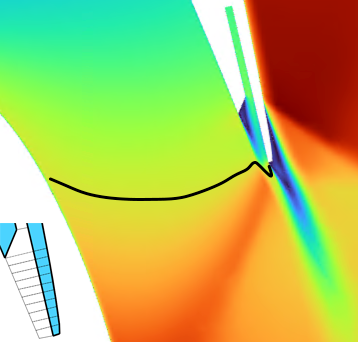
\includegraphics[width=\linewidth]{figs/ss_cutbacks_m1_lines_0.png}
		\caption{Baseline}
		\vspace{0.018\textheight}
	\end{subfigure}
	\hspace{0.05\textwidth}
	\begin{subfigure}{.42\textwidth}
		\centering
		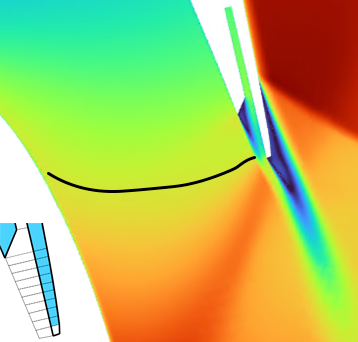
\includegraphics[width=\linewidth]{figs/ss_cutbacks_m1_lines_1.png}
		\caption{$10\%$ cutback}
		\vspace{0.018\textheight}
	\end{subfigure}
	\begin{subfigure}{.42\textwidth}
		\centering
		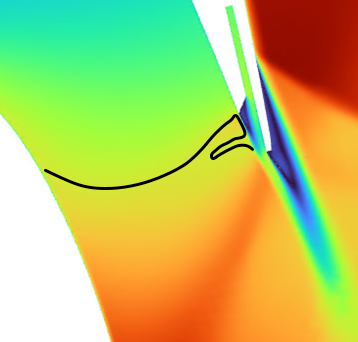
\includegraphics[width=\linewidth]{figs/ss_cutbacks_m1_lines_2.png}
		\caption{$20\%$ cutback}
	\end{subfigure}
	\hspace{0.05\textwidth}
	\begin{subfigure}{.42\textwidth}
		\centering
		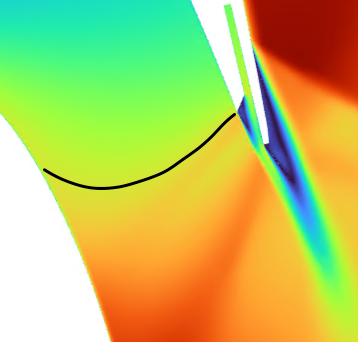
\includegraphics[width=\linewidth]{figs/ss_cutbacks_m1_lines_3.png}
		\caption{$30\%$ cutback}
	\end{subfigure}
	\begin{subfigure}{.4\textwidth}
		\centering
		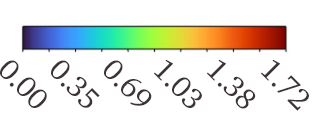
\includegraphics[width=\linewidth]{figs/mach_legend_choked_horizontal.png}
	\end{subfigure}
	\caption{Contours of Mach number showing effects of small cutbacks on the sonic line shape for Trent 900 end-edge erosion study at $\frac{p_{01}}{p_2}=3.33$}
	\label{fig:ss_cutbacks_0-3}
\end{figure}

Figure~\ref{fig:ss_cutbacks_0-3} illustrates the subtle changes in the sonic line at the nozzle exit as the nozzle guide vane's end-edge is incrementally removed until $30\%$ of its length is not present. The sonic line is shown to undergo a fundamental transition over this range of cutbacks, from initially impinging on the extremity of the end-edge in the baseline case, to impinging on the acute corner of the pressure side. It is notable that this is in direct contradiction to the commercial design philosophy which assumes the end of the cutback to define the throat in all cases. The simulated result for $20\%$ cutback suggests a sonic line attachment point which may jump between the end-edge and cutback edge in unsteady conditions.

The geometric changes are also shown to alter the aerodynamics in the suction-side region upstream of the end-edge, where an attached shock moves incrementally upstream with each increment in cutback. Shock-induced boundary layer separation is seen to be present in Figure~\ref{fig:ss_cutbacks_0-3}, and moves upstream corresponding to the position of the shock. This results in an increasingly large separated wake region which is not in alignment with the NGV's turning angle.

Figure~\ref{fig:ss_cutbacks_4-10} shows further contours of Mach number. Again the range of cutbacks is between $40\%$ and complete removal of the end-edge. Again the inverse pressure ratio is $3.3$, fully choked.

\begin{figure}[H]
	\centering
	\begin{subfigure}{.45\textwidth}
		\centering
		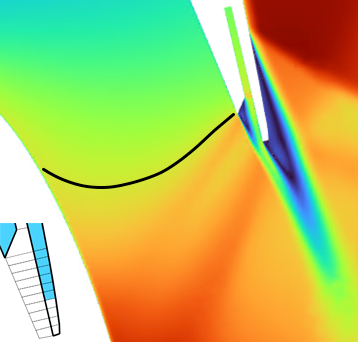
\includegraphics[width=\linewidth]{figs/ss_cutbacks_m1_lines_4.png}
		\caption{$40\%$ cutback}
		\vspace{0.018\textheight}
	\end{subfigure}
	\hspace{0.05\textwidth}
	\begin{subfigure}{.45\textwidth}
		\centering
		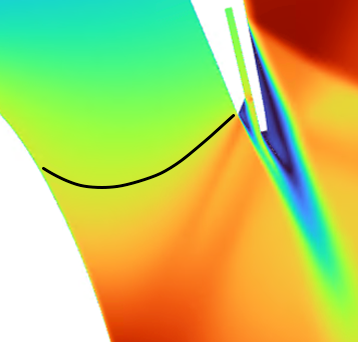
\includegraphics[width=\linewidth]{figs/ss_cutbacks_m1_lines_6.png}
		\caption{$60\%$ cutback}
		\vspace{0.018\textheight}
	\end{subfigure}
	\begin{subfigure}{.45\textwidth}
		\centering
		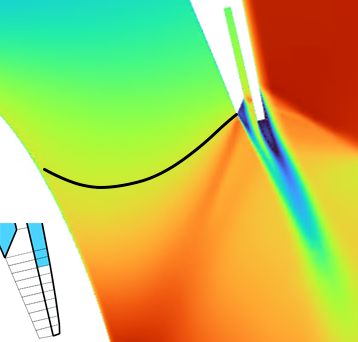
\includegraphics[width=\linewidth]{figs/ss_cutbacks_m1_lines_8.png}
		\caption{$80\%$ cutback}
	\end{subfigure}
	\hspace{0.05\textwidth}
	\begin{subfigure}{.45\textwidth}
		\centering
		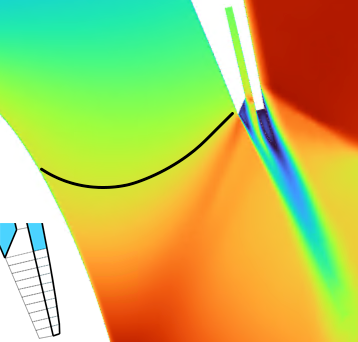
\includegraphics[width=\linewidth]{figs/ss_cutbacks_m1_lines_10.png}
		\caption{Completely cutback}
	\end{subfigure}
	\begin{subfigure}{.4\textwidth}
		\centering
		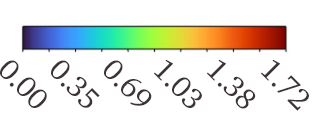
\includegraphics[width=\linewidth]{figs/mach_legend_choked_horizontal.png}
	\end{subfigure}
	\caption{Contours of Mach number showing effects of large cutbacks on the sonic line shape for Trent 900 end-edge erosion study at $\frac{p_{01}}{p_2}=3.33$}
	\label{fig:ss_cutbacks_4-10}
\end{figure}

Figure~\ref{fig:ss_cutbacks_4-10} illustrates that the shape of the sonic line is not fundamentally altered in the range between $40\%$ and $100\%$ removal of the end-edge. The sonic line is shown to consistently attach to the acute corner of the pressure side throughout this range of larger cutbacks. Upstream movement of the location of the suction-side attached shock continued to occur. This trend was reversed for the most extreme cases of $80\%$ and complete cutbacks, where the shock transitioned to a downstream location close to the corner of the end-edge, resulting in a significantly smaller separated wake region compared to other cases.

The set of Mach number contours and sonic lines suggest that the greatest sensitivity of flow capacity to end-edge cutbacks is to occur for cutbacks of $30\%$ of the end-edge or less. The sensitivity of the sonic line shape to the full range of cutbacks is illustrated in Figure~\ref{fig:ss_cutbacks_m1_lines_illustration}, which superposes the sonic lines from all simulations. It is further suggested that the location of an attached suction-side shock and corresponding boundary layer separation near the trailing edge may be sensitive to cutbacks of $40\%$ or more, but this may be imprecisely predicted by the present simulations. This is due to the lack of any observed correlation between the cutback amount and the variation in the shock location.

\begin{figure}[H]
      \centering
      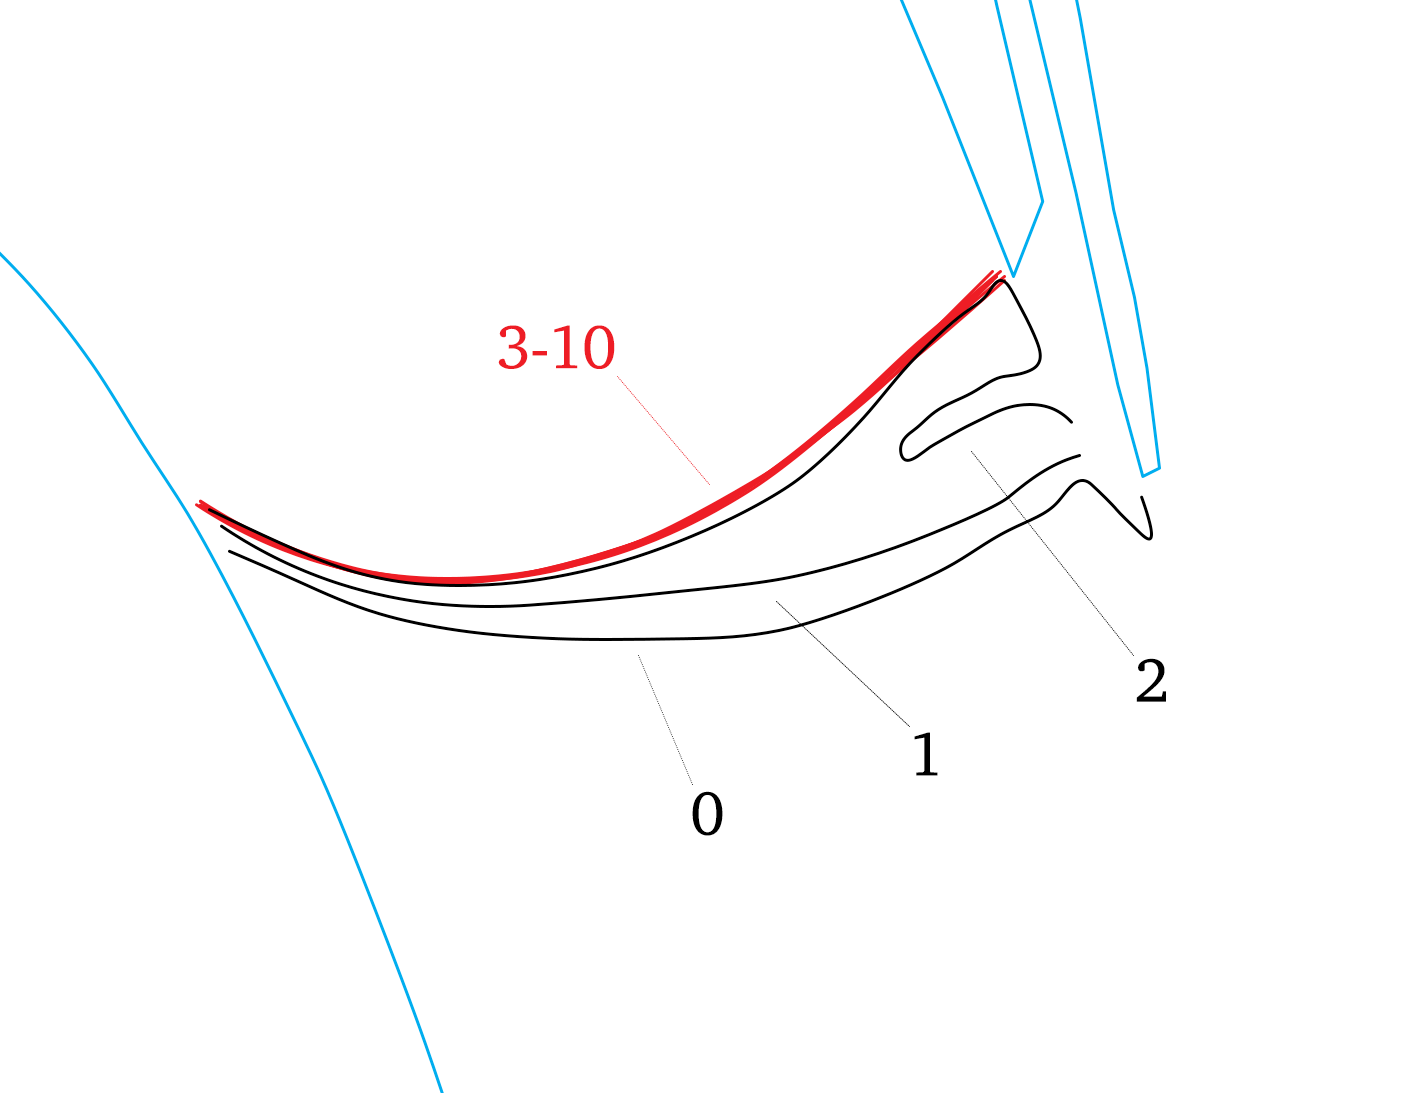
\includegraphics[width=.7\textwidth]{figs/ss_cutbacks_m1_lines_illustration.png}
      \caption{Variation in sonic line location over the full range of cutbacks for the Trent 900 end-edge erosion study, labelled by the percentage of the end-edge removed}
      \label{fig:ss_cutbacks_m1_lines_illustration}
\end{figure}

Figure~\ref{fig:ss_cutbacks_m1_lines_illustration} shows that upstream movement of the location of the suction-side attached shock occurred between $0$ and $30\%$ removal of the end-edge. This trend did not continue for cutbacks greater than $30\%$. Within this range of cutbacks, the sonic line is attached to the NGV pressure side upstream of the cooling slot, as there is insufficient length over which reattachment can occur downstream. This is a useful result for the engine designer, as it provides a stable end-of-life capacity prediction for the NGV.

Figure~\ref{fig:ss_cutbacks_vs_capacities_pressure_ratios} plots flow capacity change as a function of the amount of the end-edge that has been removed. The trend is plotted for 3 inverse pressure ratios: $1.50$, the design value of $1.79$, and a fully choked value of $3.33$.

\begin{figure}[H]
	\centering
	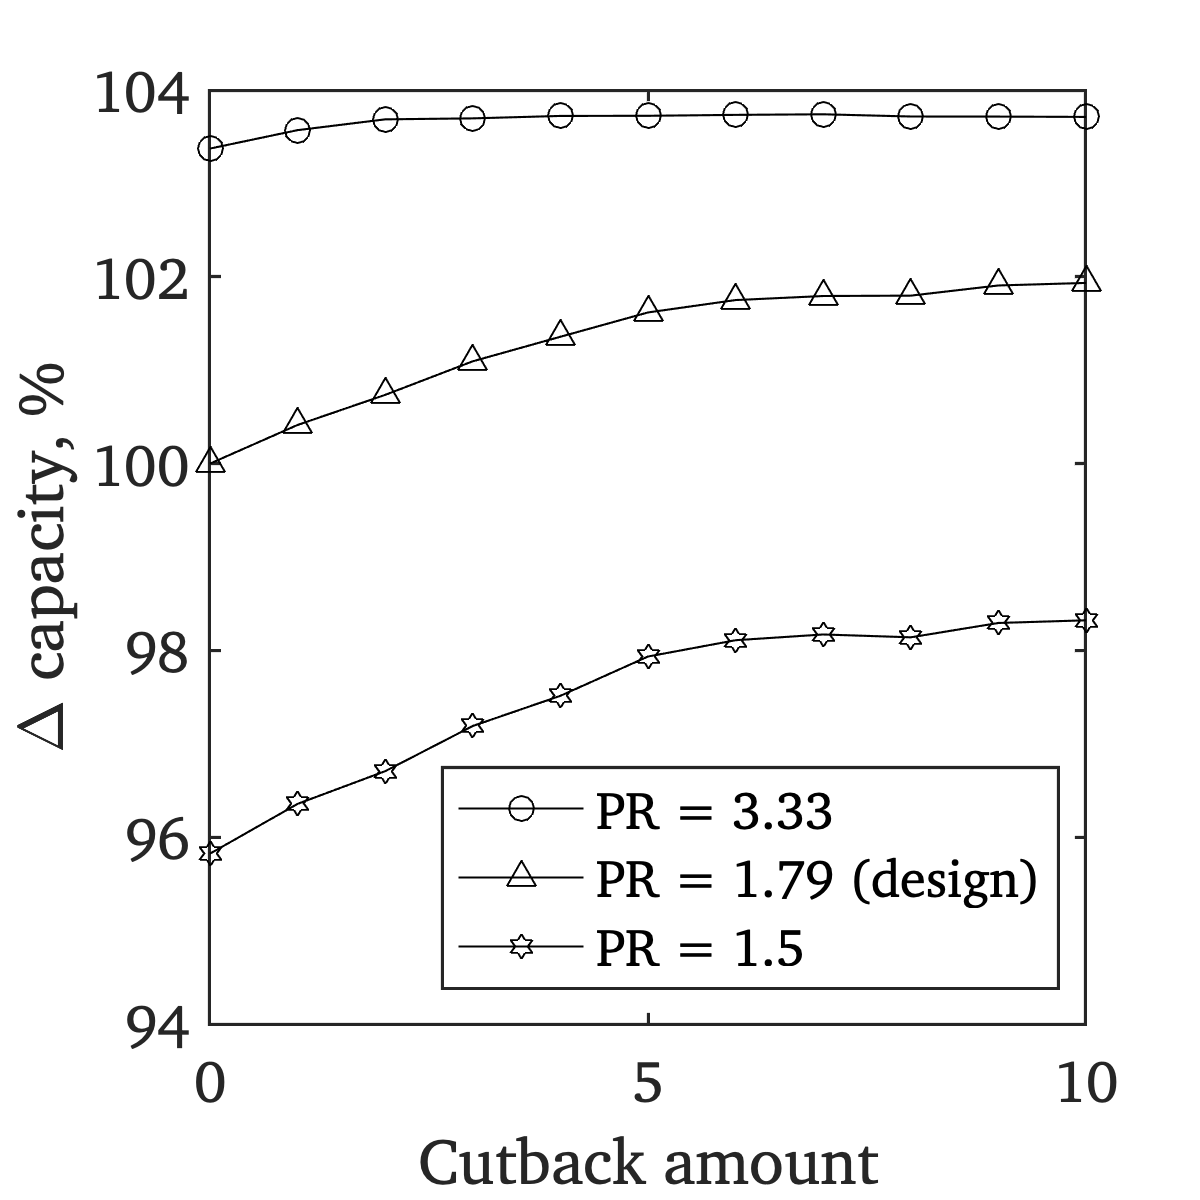
\includegraphics[width=.45\textwidth]{figs/ss_cutbacks_vs_capacities_pressure_ratios.png}
	\caption{2D capacity percentage delta as a function of end-edge cutback amount for a Trent 900 NGV at $\frac{p_{01}}{p_2}=1.5$, $1.79$ (design), and $3.33$}
    \label{fig:ss_cutbacks_vs_capacities_pressure_ratios}
\end{figure}

At an inverse pressure ratio of $3.33$, Figure~\ref{fig:ss_cutbacks_vs_capacities_pressure_ratios} shows a relationship between flow capacity and cutback amount which is in good agreement with the observations made from the corresponding sonic line visualisations. Capacity is shown to be sensitive to cutback amounts of $0$, $10\%$, and $20\%$, and insensitive to cutbacks thereafter. The corresponding sonic lines are observed to vary in shape when capacity varies, and to remain similar in shape when capacity does not vary. The observed switching of the sonic line from the end-edge-attached mode (at baseline) to the pressure-side-attached mode (at cutbacks of $30\%$ and greater) is associated with a $0.3$ percentage point increase in capacity. For all cutbacks subsequent to the mode switch, there is no capacity change at this pressure ratio. This is in good agreement with the discussion in Chapter~\ref{chapter_geometric_throat_area} which concluded that the effective throat area of a fully choked nozzle guide vane is predominantly a function of the shape of its sonic line.

At lower inverse pressure ratios where the flow is not fully choked, and thus a sonic line cannot be drawn, flow capacity varied over a significantly greater range of cutback percentage. This is to be expected by consideration of choked versus unchoked compressible flows as discussed earlier in this section. This discussion implies that, in the general case of compressible flow in 2D nozzles, the nozzle flow capacity will increase if the effective passage width is increased at any point along the nozzle. However, this is also a consequence of providing less turning in the flow. An entirely unturned flow would have maximum capacity in the annular cross-section that is the gas turbine. 

This is in good agreement with the observed relationship between flow capacity and cutback amount at the unchoked pressure ratios. Removal of end-edge material increases the effective passage width in the region local to the end-edge, causing a local decrease in static pressure and increase in dynamic pressure. Because most streamlines are unchoked at the flow region and pressure ratios in question, this state change propagates along the entire streamline with a corresponding increase in mass flow rate.

The maximum change in capacity was $1.9$ percentage points at the design inverse pressure ratio of $1.79$, and $2.5$ percentage points at an inverse pressure ratio of $1.50$. The effect of increasing cutbacks became less pronounced at larger cutback amounts, suggesting that the size of the end-edge ceases to be the limiting factor on effective passage width for those geometries. Figure~\ref{fig:ss_cutbacks_wakes_design_pr} shows contours of Mach number in the NGV wake region for the full range of cutbacks at the design inverse pressure ratio of $1.79$, labelled by the percentage of the end-edge removed.

\begin{figure}[H]
	\centering
	\begin{subfigure}{.9\textwidth}
		\centering
		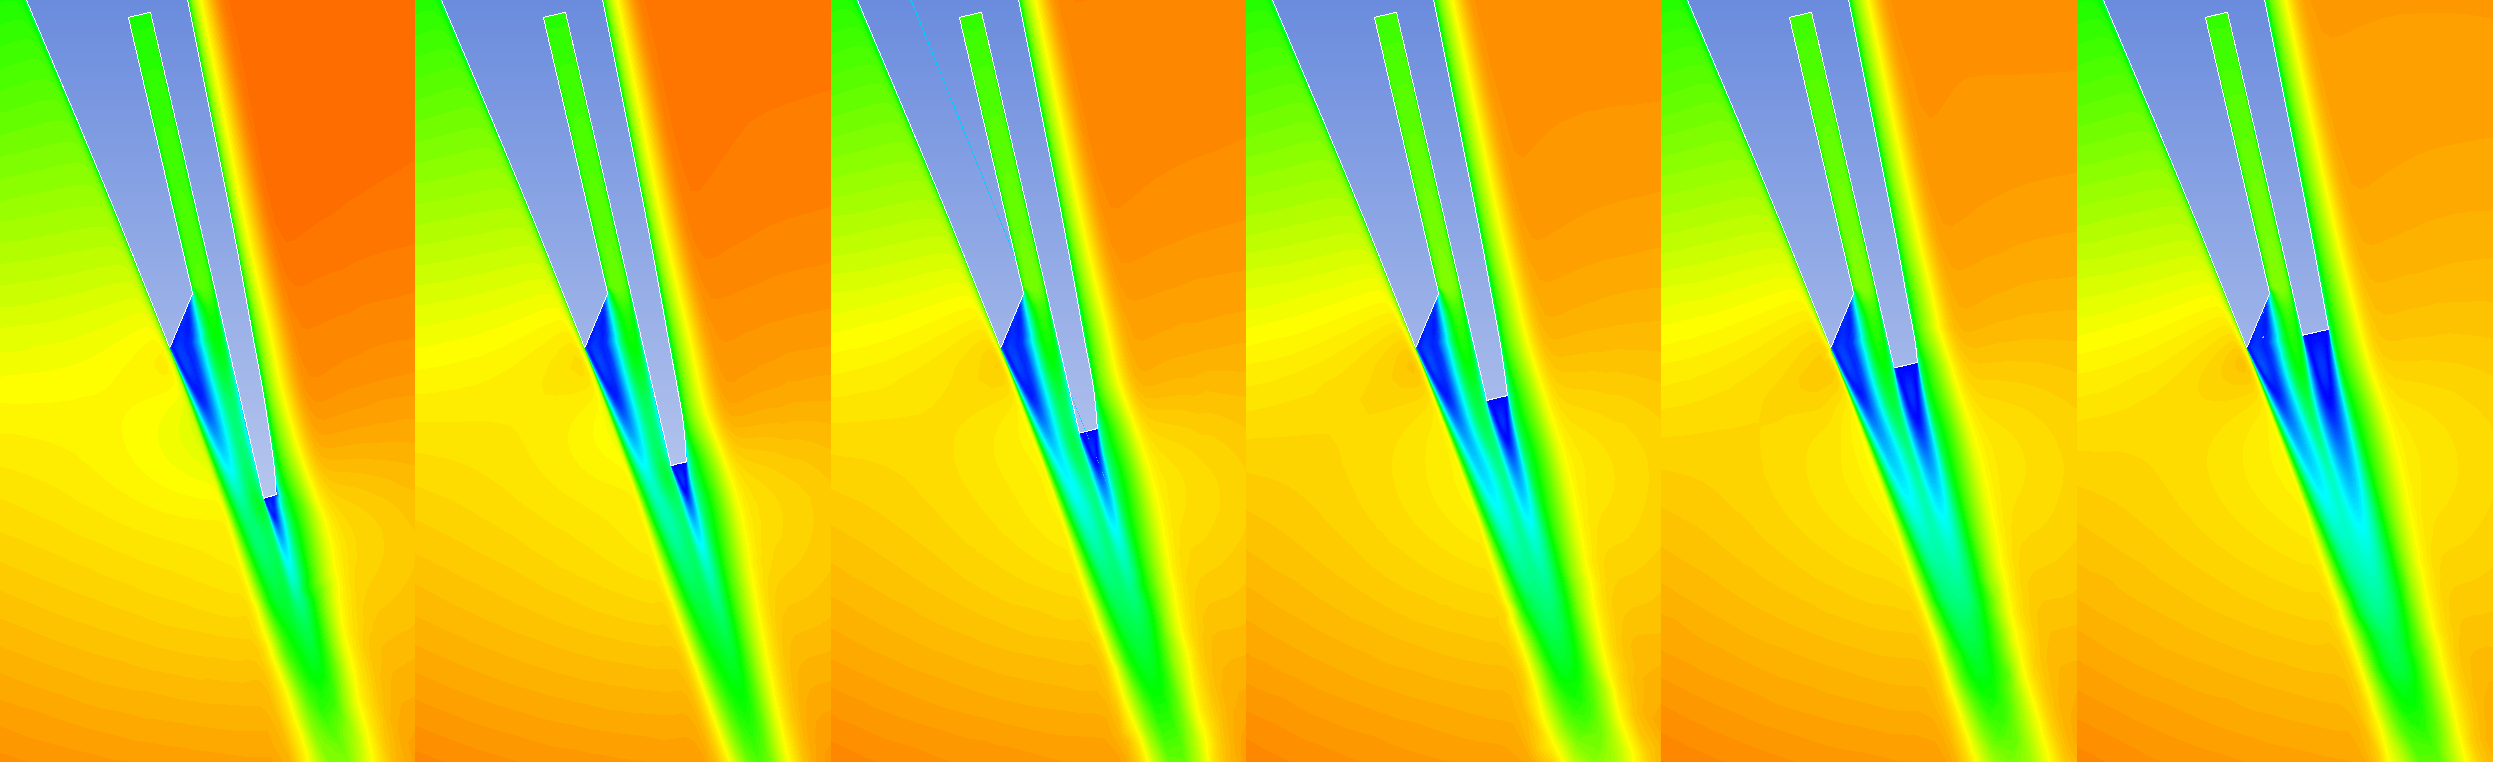
\includegraphics[width=\linewidth]{figs/ss_cutbacks_wakes_design_pr.png}
	\end{subfigure}
	\begin{subfigure}{.4\textwidth}
		\centering
		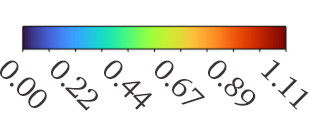
\includegraphics[width=\linewidth]{figs/mach_legend_design_horizontal.png}
	\end{subfigure}
	\caption{Contours of Mach number in the wake region of the Trent 900 end-edge erosion study at $\frac{p_{01}}{p_2}=1.79$ (design), labelled by percent of the end-edge removed}
      \label{fig:ss_cutbacks_wakes_design_pr}
\end{figure}

Key features of Figure~\ref{fig:ss_cutbacks_wakes_design_pr} include an outer wake region (rendered in green) and inner wake regions downstream of the pressure side and the end-edge (rendered in blue). No fundamental changes occurred to the trailing edge's aerodynamics over the range of cutbacks. Mach number is observed to continually increase in the region adjacent to the pressure side, and to continually decrease in the region adjacent to the end-edge. The trailing edge aerodynamics were sensitive to geometric changes across the full range of cutbacks. The reduced effect of greater cutbacks on flow capacity may result from two phenomena. Firstly, the local flow acceleration may be limited more by the position of the pressure side than by the end-edge at higher cutback values, where the end-edge tip is increasingly too far upstream to influence the pressure-side aerodynamics. Secondly, this upstream positioning of the end-edge tip is observed to cause a significant increase in outer wake thickness at higher cutback values. This likely reduced the effective passage width in this region and counteracted the predominant effect of flow capacity increasing.

Figure~\ref{fig:ss_cutbacks_vs_capacities_trends} plots trends of flow capacity change versus inverse pressure ratio at selected cutback amounts. The range of inverse pressure ratios includes the design value of $1.79$. Capacity changes are normalised against the case of $0$ cutback at the design pressure ratio.

\begin{figure}[H]
	\centering
	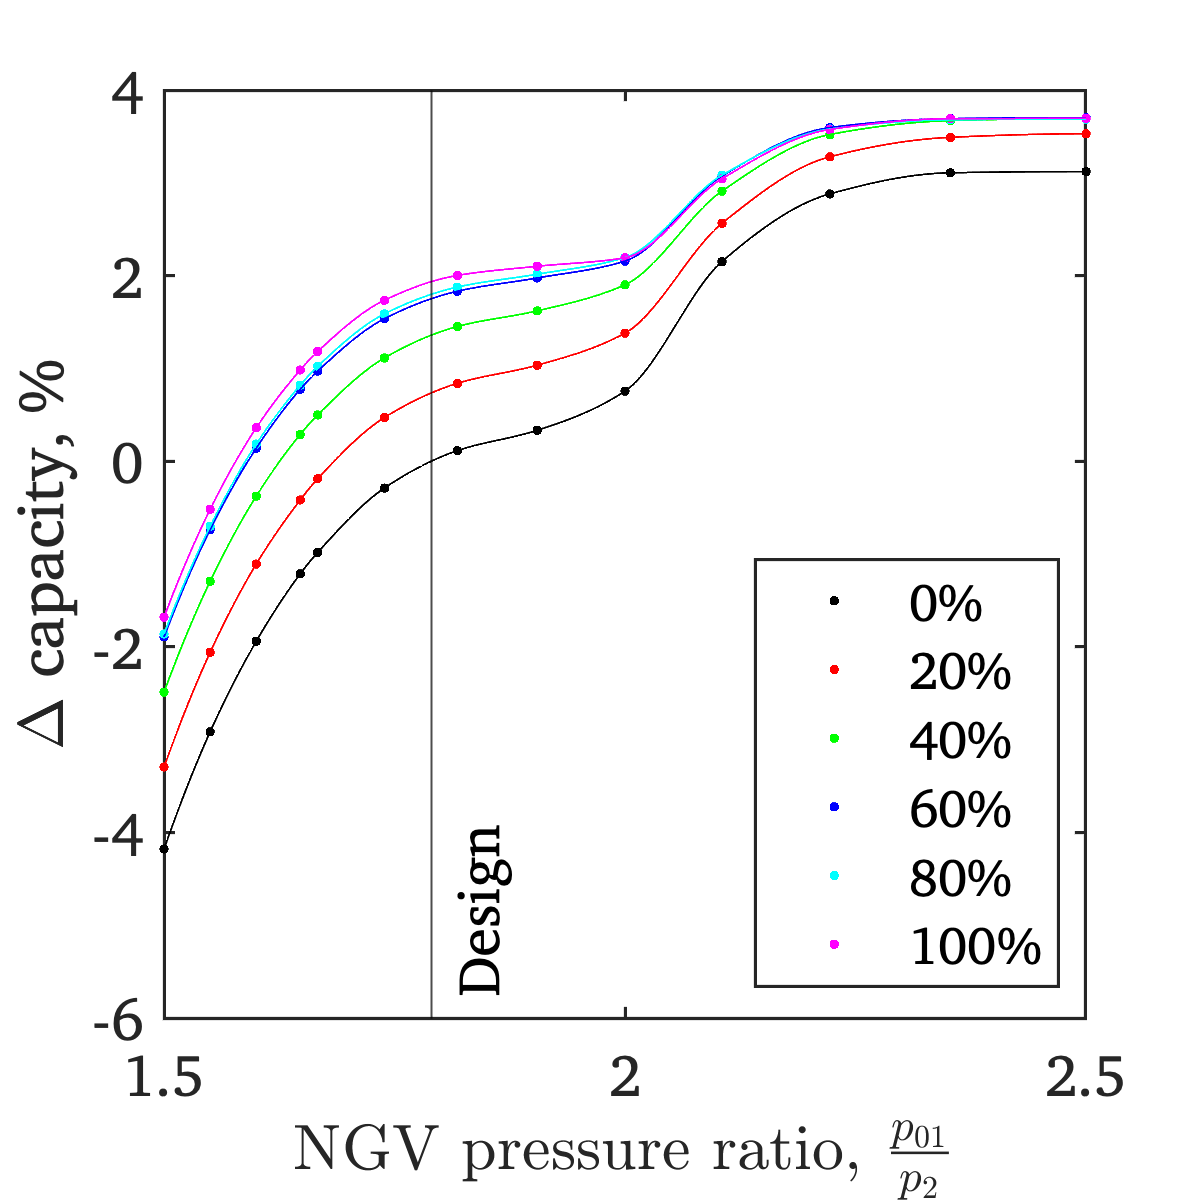
\includegraphics[width=.45\textwidth]{figs/ss_cutbacks_vs_capacities_trends.png}
	\caption{2D normalised capacity as a function of pressure ratio for a Trent 900 NGV over the full range of end-edge cutbacks}
    \label{fig:ss_cutbacks_vs_capacities_trends}
\end{figure}

In terms of the effects of cutbacks on flow capacity, Figure~\ref{fig:ss_cutbacks_vs_capacities_trends} is in good agreement with Figure~\ref{fig:ss_cutbacks_vs_capacities_pressure_ratios}. The capacity delta produced by full end-edge removal continuously decreased with increasing inverse pressure ratio, and the capacity trends remained qualitatively similar for all cutback amounts. These observations suggest that the cutback-induced capacity changes and the onset of choking are 2 independent phenomena which do not influence each other. It is concluded that, as inverse pressure ratio increased, more streamlines became choked and ceased to be affected by cutbacks downstream of those streamlines' sonic points. 

It is further concluded that the capacity trend shapes and onsets of choking were unaffected by variable cutbacks, but remained a function of only inverse pressure ratio. This is likely due to the relevant geometric changes taking place downstream of the throat region. This is complementary to the results of Chapter~\ref{chapter_geometric_throat_area}, where geometric changes upstream of the throat resulted in qualitatively distinct capacity trends and dissimilar onsets of choking.

\subsection{Effect on performance}

Simulation data were also used to evaluate the aerodynamic penalties associated with the incremental cutbacks to the end-edge at the design inverse pressure ratio of $1.79$. These penalties include the change to the NGV's ability to turn the flow by the correct angle, and the effect of the cutbacks on the NGV loss.

Velocity components at the domain outlet were surveyed and mass-averaged over the length of the outlet. This resulted in a value for mean NGV turning angle for each incremental cutback. Figure~\ref{fig:ss_cutbacks_vs_turning_angles} plots turning angle deviation in degrees versus end-edge cutback amount.

\begin{figure}[H]
	\centering
	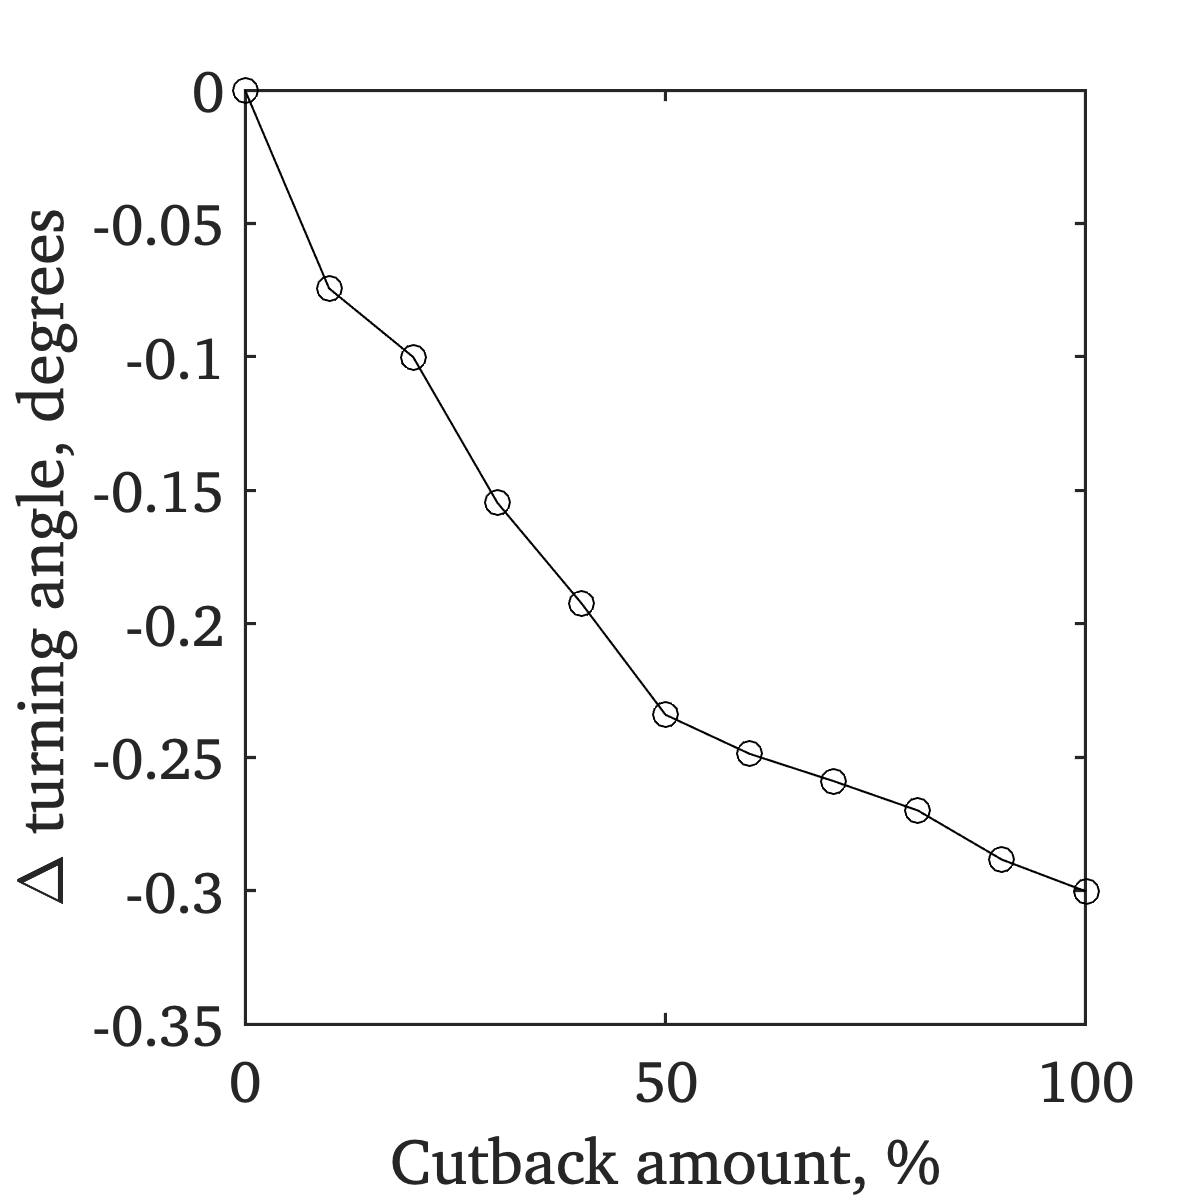
\includegraphics[width=.45\textwidth]{figs/ss_cutbacks_vs_turning_angles.png}
	\caption{NGV turning angle delta as a function of end-edge cutback amount for a Trent 900 NGV at $\frac{p_{01}}{p_2}=1.79$}
    \label{fig:ss_cutbacks_vs_turning_angles}
\end{figure}

Figure~\ref{fig:ss_cutbacks_vs_turning_angles} shows that the NGV's ability to turn the flow was significantly reduced as cutbacks increased. Complete removal of the end-edge resulted in a turning angle reduction of $0.3$ degrees, with increased sensitivity to cutbacks at smaller cutback amounts. This trend is unsurprising. If no vane were present, this would equate to no turning. For the high-pressure turbine downstream of the NGV, reduced turning equates to less available work and additional loss at entry to the rotor.

Overall flow turning angle was surveyed along the length of the domain outlet plane. Figure~\ref{fig:ss_cutbacks_turning_angle_surveys} plots this distribution of turning angles at selected cutback amounts. On the outlet plane, $0\rightarrow1$ denotes travel in the negative $y$ direction, which is the direction the flow turns. Stations $0$ and $1$ are labelled on the illustration of the computational domain in Chapter~\ref{chapter_geometric_throat_area}, Figure~\ref{fig:computational_domain_and_boundaries}. Station $0.5$ corresponds to the geometric extrapolation of the NGV trailing edge to the outlet plane.

\begin{figure}[H]
	\centering
	\begin{subfigure}{.125\textwidth}
		\centering
		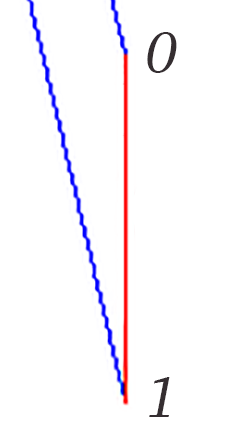
\includegraphics[width=\linewidth]{figs/outlet_minifigure.png}
	\end{subfigure}
	\begin{subfigure}{.45\textwidth}
		\centering
		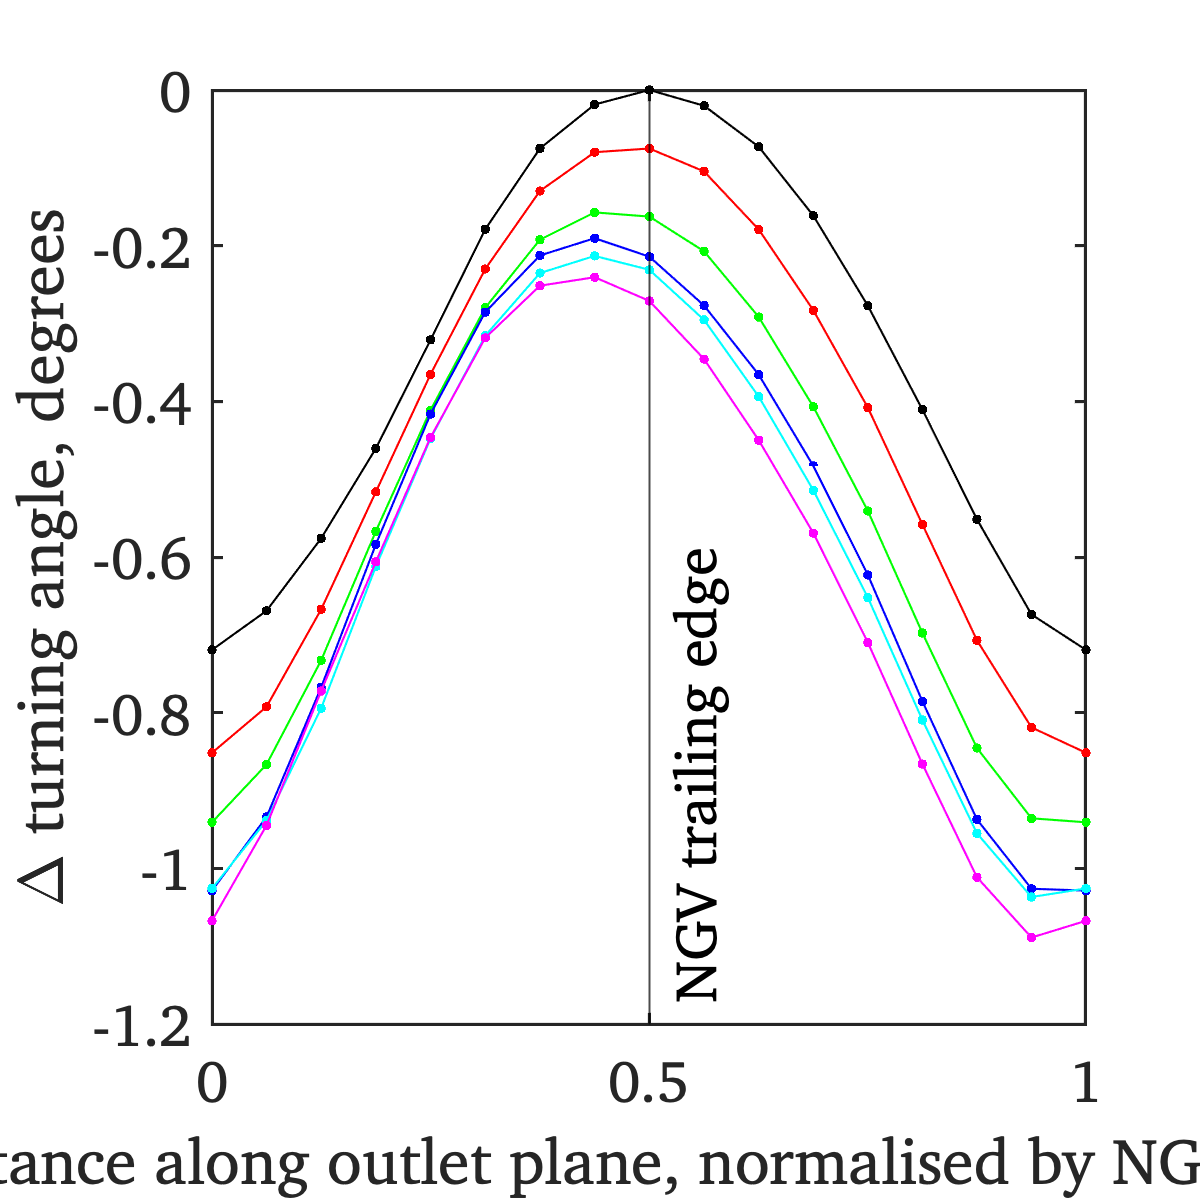
\includegraphics[width=\linewidth]{figs/ss_cutbacks_turning_angle_surveys.png}
	\end{subfigure}
	\begin{subfigure}{.1125\textwidth}
		\centering
		
\includegraphics[width=\linewidth]{figs/ss_cutbacks_vs_capacities_trends_legend_ver02.png}
	\end{subfigure}
	\caption{Outlet plane turning angle surveys over the full range of cutbacks for the Trent 900 end-edge erosion study at $\frac{p_{01}}{p_2}=1.79$}
      \label{fig:ss_cutbacks_turning_angle_surveys}
\end{figure}

Figure~\ref{fig:ss_cutbacks_turning_angle_surveys} further illustrates the trend of reducing turning angles present in Figure~\ref{fig:ss_cutbacks_vs_turning_angles}. It is also apparent that the incremental cutbacks caused a shift in the location of maximum turning angle. In the case of no cutback, maximum turning occurred exactly halfway across the domain exit plane, at a location immediately downstream of the NGV end-edge. Subsequent cutbacks caused both a reduction in maximum turning and a shift of the maximum turning location in the opposite direction to which turning occurs. This suggests that the NGV wake continued to extend downstream of the NGV at an angle which decreased with increasing cutbacks, arriving at the domain outlet at an incrementally increasing $y$-coordinate. Assuming that the downstream turning angle distribution is indicative of the NGV wake profile, the wake did not appear to become significantly more diffuse as cutbacks increased.

Figure~\ref{fig:ss_cutbacks_vs_losses} plots loss as a function of end-edge cutback amount at the design pressure ratio of $1.79$, where total pressure loss and kinetic energy loss are defined as in Section~\ref{definitions_of_loss}. Total pressure values were surveyed at the domain outlet plane and averaged to produce the loss values.

\begin{figure}[H]
	\centering
	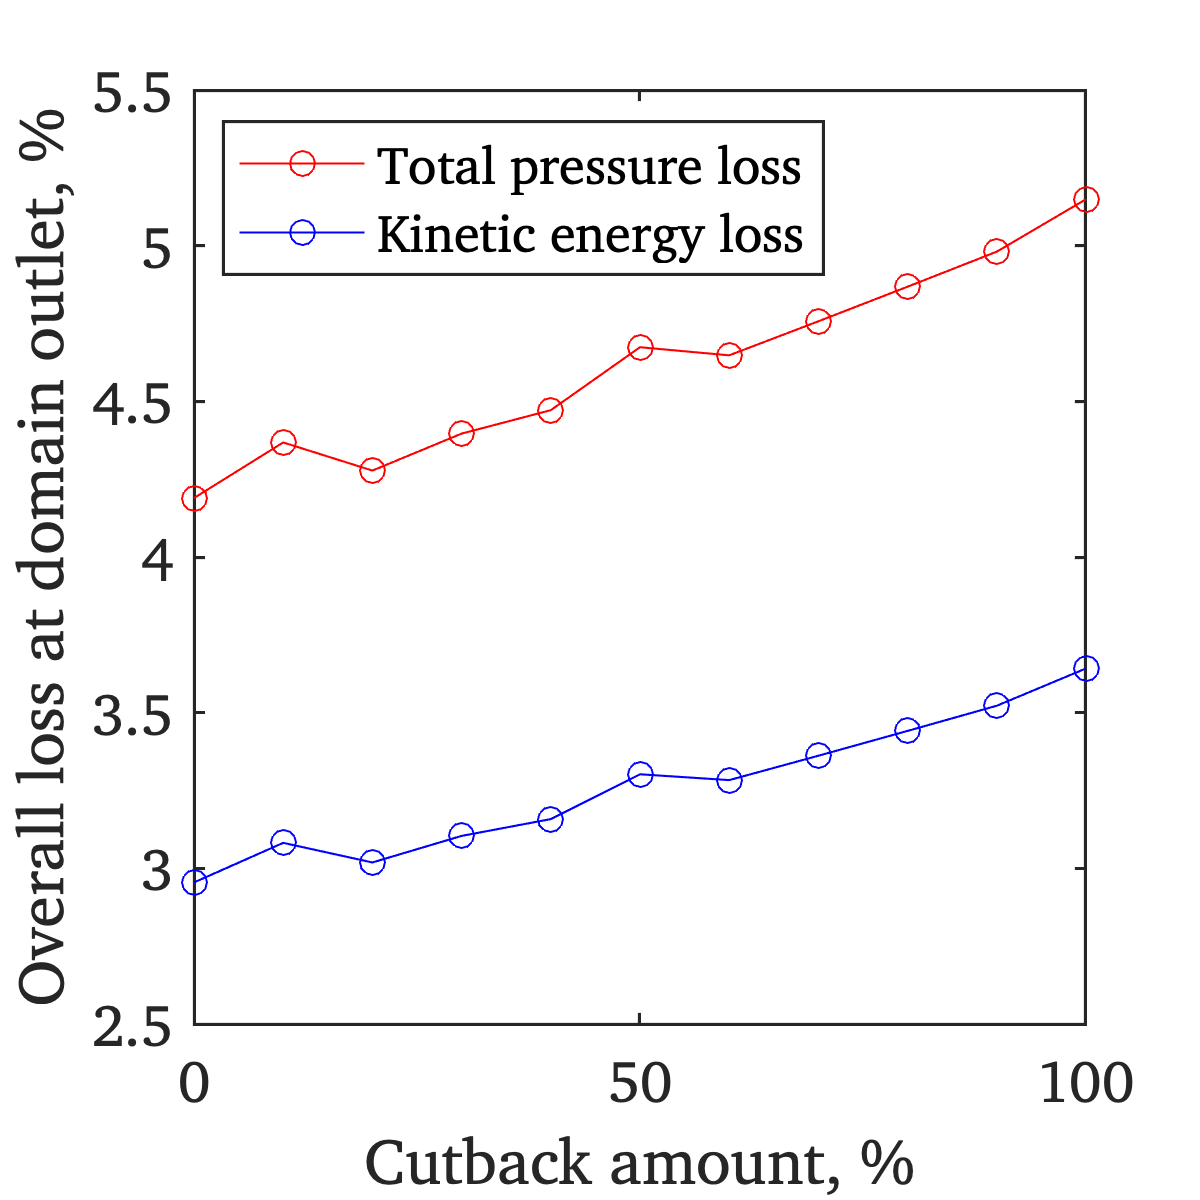
\includegraphics[width=.45\textwidth]{figs/ss_cutbacks_vs_losses.png}
	\caption{Loss as a function of end-edge cutback amount for a Trent 900 NGV at $\frac{p_{01}}{p_2}=1.79$}
    \label{fig:ss_cutbacks_vs_losses}
\end{figure}

Figure~\ref{fig:ss_cutbacks_vs_losses} shows that both types of loss increased with incremental cutbacks. Total pressure loss was observed to increase by approximately $1\%$ over the range of cutbacks, and kinetic energy loss by approximately $0.7\%$. This is in agreement with the discussion of figure~\ref{fig:ss_cutbacks_wakes_design_pr} which suggested that loss would likely be incurred by the increasing area of separated wake that occurs as cutbacks increase. This effect may be exacerbated by the deviation from the design turning angle that also occurs, whereby the NGV wake is deflected in the positive $x$-coordinate with corresponding increase in its area.

Loss delta is plotted as a function of capacity delta in Figure~\ref{fig:ss_capacities_vs_losses}. This plot covers the range of incremental cutbacks and is for the design inverse pressure ratio of $1.79$.

\begin{figure}[H]
	\centering
	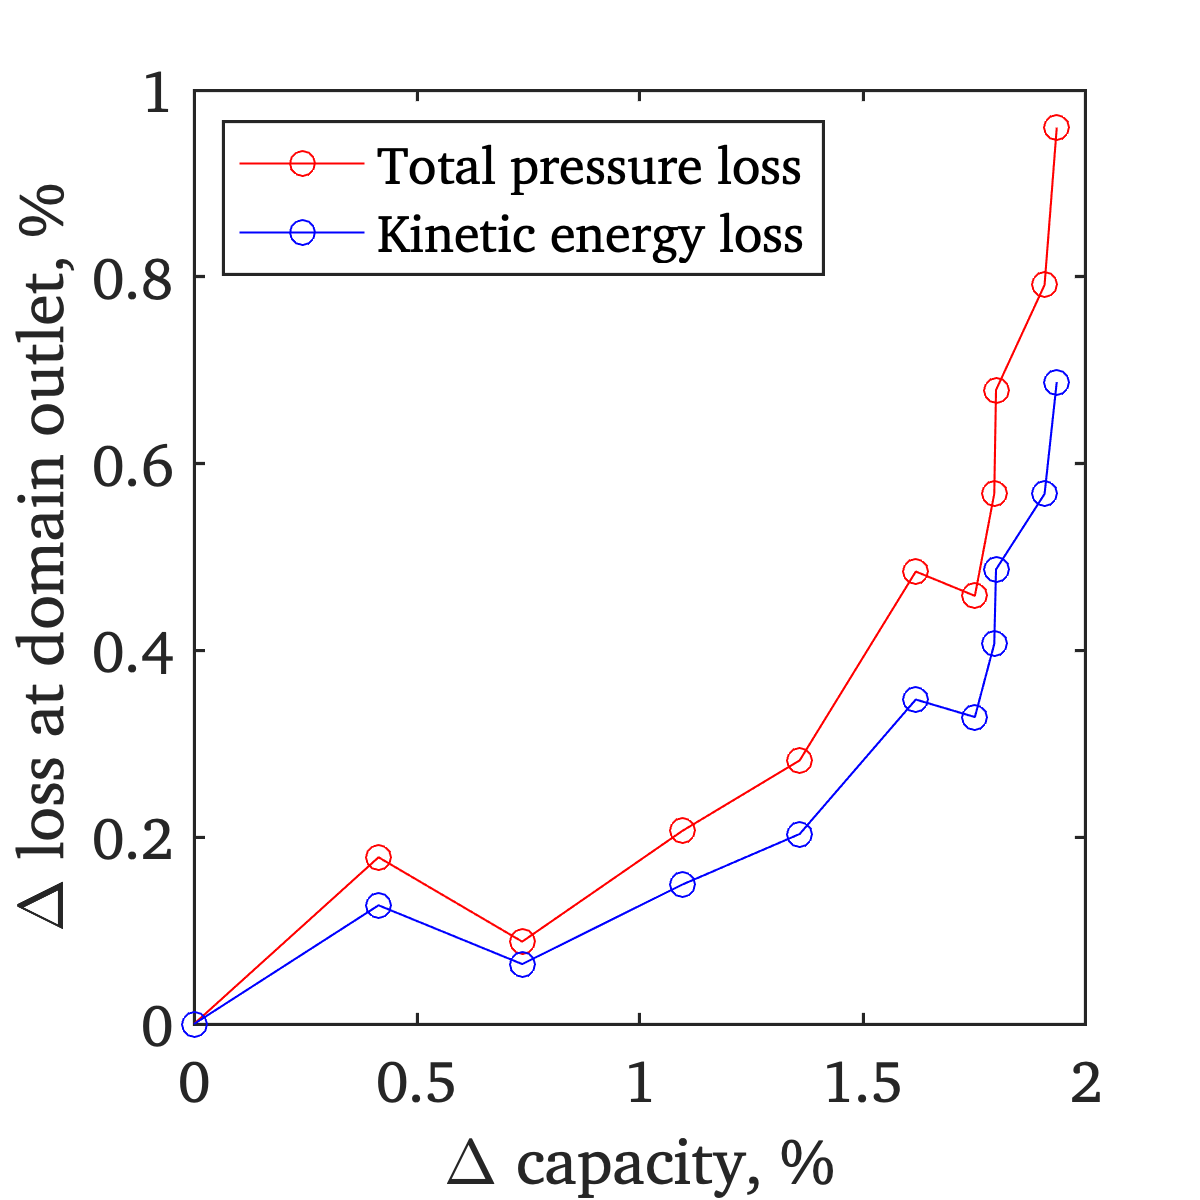
\includegraphics[width=.45\textwidth]{figs/ss_capacities_vs_losses.png}
	\caption{Loss delta as a function of capacity delta over the full range of cutbacks for the Trent 900 end-edge erosion study at $\frac{p_{01}}{p_2}=1.79$}
    \label{fig:ss_capacities_vs_losses}
\end{figure}

Figure~\ref{fig:ss_capacities_vs_losses} shows that, as the end-edge is incrementally removed, capacity and loss do not change in direct proportion to each other. Although overall capacity sensitivity was greater than overall loss sensitivity, at higher cutback amounts a relatively small increase in capacity corresponded to a sharp increase in loss by both definitions. In agreement with this section's previous analysis of the capacity and loss mechanisms present across the range of cutbacks, it is concluded that capacity sensitivity is of greatest concern in cases of relatively small erosion of the NGV end-edge, and loss sensitivity is of concern in all cases but especially in cases of relatively large erosion.






\section{Effects of pressure-side trailing edge sizing}
\label{performance_of_an_alternative_trailing_edge_design}
%--Centred-ejection option (PS cutbacks) (and could it reduce loss) and what happens as its geometry is changed to gradually look more like an existing design
%--We must also consider broader TE manufacturing changes that are likely to happen on purpose - the switch to CMC manufacturing of turbine blades. How will this change the game, and what tolerances are expected?

This section considers the location of the pressure-side cutback that is present on the NGV. This feature is required to prevent blockage of the coolant supply to the end-edge, which would be damaged very rapidly by oxidation erosion if the slot coolant flow were not present. Although the pressure side could be extended further downstream into a thinner feature with a smaller wake, the cutback prevents blockage of the slot coolant flow by causing it to form an external film attached to the pressure side of the end-edge. If a coolant blockage is present upstream inside the vane, the end-edge coolant film will remain relatively unchanged after mixing with itself.

Improved materials and manufacturing techniques may necessitate alternative trailing edge geometries. Giel et al~\cite{giel_te_thickness} noted that ``in the pursuit of higher turbine inlet temperatures for reduced fuel burn and emissions consistent with NASA's goals~\cite{giel_nasa_reference}, Ceramic Matrix Composite (CMC) materials are now being implemented in gas turbine engines...They enable higher turbine inlet temperatures, thus enabling higher overall pressure ratios (OPRs) for the engine and higher thermal efficiency.'' 

The authors used a linear cascade to measure the aerodynamic performance of a set of blades representing the geometric constraints of the CMC manufacturing method. Of main concern was the constraint that ``the trailing edge thicknesses of CMC blades are anticipated to be significantly larger than those of current state-of-the-art metallic blades,'' which may be expected to cause increased loss.

\subsection{Geometry, mesh, and boundary conditions}

The larger the pressure-side cutback, the less the likelihood of coolant blockage, and the easier it is to perform the machining of the trailing edge. However, a bigger cutback is expected to cause increased loss due to increased wake area, although the limiting design factor is the reduction in film cooling effectiveness on the end-edge as the coolant becomes mixed out. With enough mixing, there would eventually be no cooling potential in the film cooling flow. This section presents a 2D CFD study on varying the size of the pressure-side cutback, using the types of analyses presented for end-edge cutbacks in Section~\ref{suction_side_cutbacks}. The baseline geometry included a partially eroded end-edge to be representative of the full lifetime of the component, for which a cutback amount of approximately $50\%$ was chosen. The baseline pressure-side cutback was such that the pressure side and the suction side extended by the same amount, with no end-edge. Cutbacks were then made to move the end of the pressure side upstream in increments of $25\%$, where $100\%$ is equivalent to the existing location of the pressure side of the trailing edge. The process of geometry refinement is illustrated in Figure~\ref{fig:t900_ps_cutbacks_geometry}.

\begin{figure}[H]
	\centering
	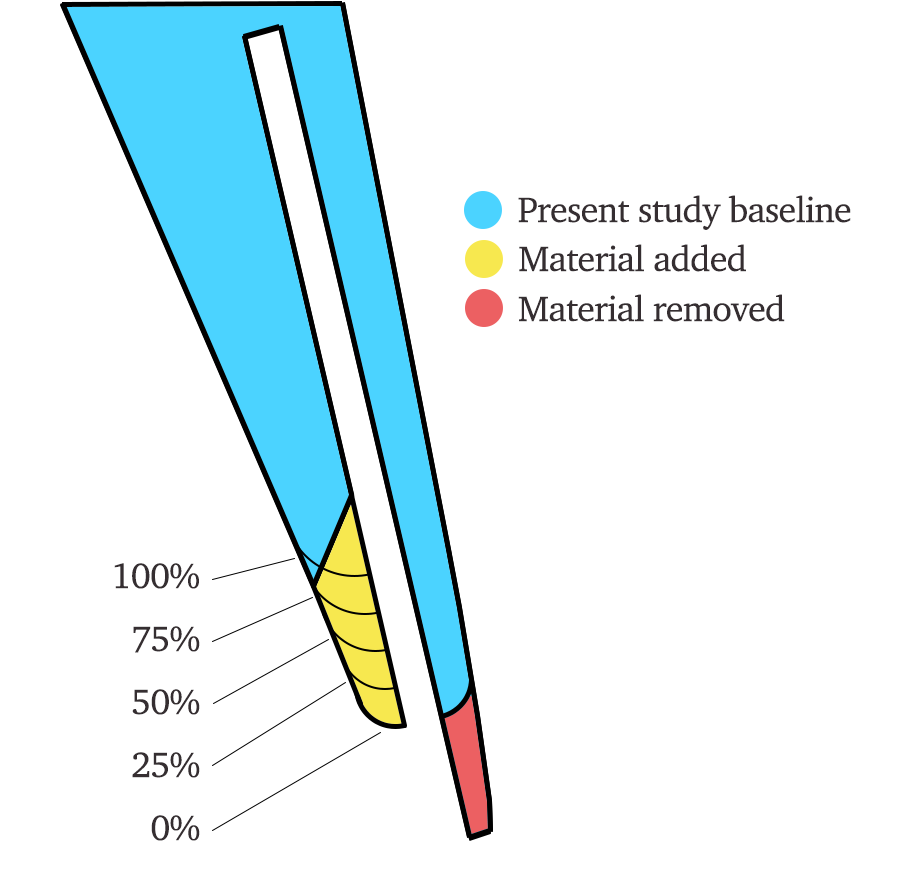
\includegraphics[width=.60\textwidth]{figs/t900_ps_cutbacks_geometry.png}
	\caption{Geometry processing scheme for cutbacks to the pressure side of a Trent 900 NGV}
    \label{fig:t900_ps_cutbacks_geometry}
\end{figure}

As in Section~\ref{suction_side_cutbacks}, simulations were performed at a range of inverse pressure ratios between 1.5 and 3.33, and particular study was made at inverse pressure ratios of 1.5, 1.79 and 3.33. 1.79 is the design cruise condition for the Trent 900 engine. Boundary conditions were as described in Table~\ref{ss_cutbacks_parameters}.

This geometry did not allow for the approach of Section~\ref{suction_side_cutbacks} where material was replaced with structured fluid mesh. For this geometry, an additional structured quadrilateral mesh block was created for cutback sizes greater than 0. This block deformed as cutbacks were increased, maintaining element spacing on the outer edge of the structured boundary layer mesh region. The sizing of this region was consistent with that used in Section~\ref{suction_side_cutbacks}, as was the design of the unstructured quadrilateral mesh for the overall domain. Figure~\ref{fig:t900_ps_cutbacks_meshes} depicts the meshes used for the cases of $0\%$, $25\%$, $50\%$, and $75\%$ cutbacks.

\begin{figure}[H]
	\centering
	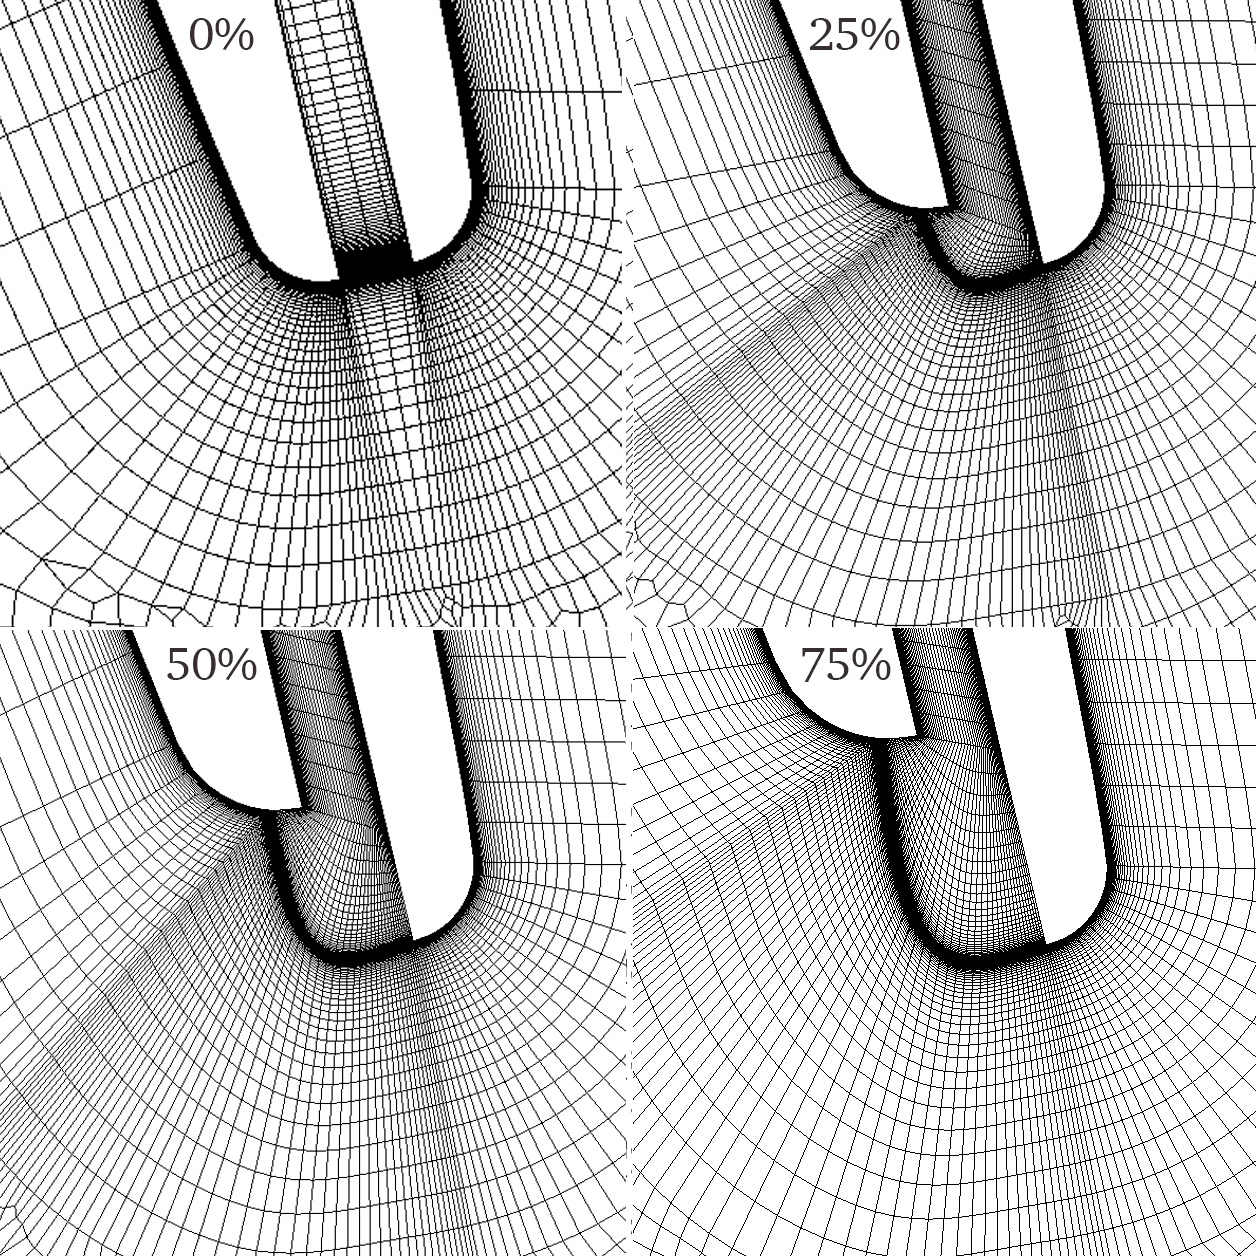
\includegraphics[width=.60\textwidth]{figs/T900_ps_cutbacks_meshes.png}
	\caption{Examples of meshes for cutbacks to the pressure side of a Trent 900 NGV}
    \label{fig:t900_ps_cutbacks_meshes}
\end{figure}

In Figure~\ref{fig:t900_ps_cutbacks_meshes}, deformation of the bottom edge of the aforementioned mesh block is prominently visible due to the continuation of the laminar sublayer resolution around the circumference of the vane, which requires it to bridge the gap across the trailing edge slot. The described mesh, geometry alteration strategy, and boundary conditions were used to perform 5 CFD simulations which incrementally spanned the range of cutbacks between the described baseline and a fully cut back pressure side. Solutions were initialised using the solver's built-in FMG initialisation and Journal scripts as described in Section~\ref{section_1d_vs_2d_capacity_uncertainty}. NGV mass flow rate was saved at each pressure ratio. Full solution data were saved for the final fully choked pressure ratio to enable analysis of the shocks, expansions and sonic line at choked conditions. There were 32 increments of pressure ratio, and typical overall solution times were approximately 10 hours. The k-$\omega$ SST turbulence model was used.

\subsection{Effect on capacity}

Figure~\ref{fig:ps_cutbacks_choked} shows contours of Mach number in the region of the trailing edge for the described study. The depicted range of cutbacks is between $0\%$ and $100\%$. Inverse pressure ratio is $3.33$, fully choked.

\begin{figure}[H]
	\centering
	\begin{subfigure}{.42\textwidth}
		\centering
		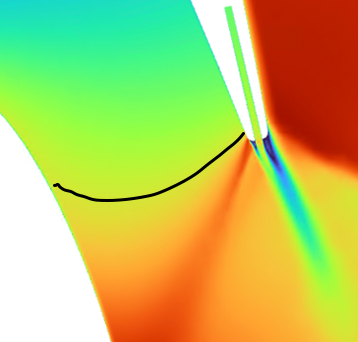
\includegraphics[width=\linewidth]{figs/ps_cutbacks_choked_0.png}
		\caption{Baseline}
		\vspace{0.018\textheight}
	\end{subfigure}
	\hspace{0.05\textwidth}
	\begin{subfigure}{.42\textwidth}
		\centering
		\includegraphics[width=\linewidth]{figs/ps_cutbacks_choked_25.png}
		\caption{$25\%$ cutback}
		\vspace{0.018\textheight}
	\end{subfigure}
	\begin{subfigure}{.42\textwidth}
		\centering
		\includegraphics[width=\linewidth]{figs/ps_cutbacks_choked_50.png}
		\caption{$50\%$ cutback}
		\vspace{0.018\textheight}
	\end{subfigure}
	\hspace{0.05\textwidth}
	\begin{subfigure}{.42\textwidth}
		\centering
		\includegraphics[width=\linewidth]{figs/ps_cutbacks_choked_75.png}
		\caption{$75\%$ cutback}
		\vspace{0.018\textheight}
	\end{subfigure}
	\begin{subfigure}{.15\textwidth}
		\centering
		\includegraphics[width=\linewidth]{figs/mach_legend_choked.png}
	\end{subfigure}
	\begin{subfigure}{.42\textwidth}
		\centering
		\includegraphics[width=\linewidth]{figs/ps_cutbacks_choked_100.png}
		\caption{$100\%$ cutback}
	\end{subfigure}
	\caption{Contours of Mach number in the wake region of the Trent 900 pressure-side cutback study at $\frac{p_{01}}{p_2}=3.33$, labelled by percent of the pressure side removed}
	\label{fig:ps_cutbacks_choked}
\end{figure}

Figure~\ref{fig:ps_cutbacks_choked} illustrates that the sonic line moved incrementally upstream with increasing pressure-side cutbacks. The sonic line remained attached to the pressure side of the trailing edge at a point just upstream of where boundary layer separation occurred, and this remained true as both the pressure side and the sonic line progressed upstream as cutbacks increased. On the suction side of the adjacent vane, the sonic line attached at a point that also moved incrementally upstream. In all cases, a shock was present immediately upstream of the point of pressure-side boundary layer separation, which was in a region of high convex curvature on the vane surface. Shock-induced boundary layer separation also occurred on the suction side of the trailing edge at a location that was not affected by the incremental changes to the pressure side. In cases of $25\%$ cutback or more, an additional shock appeared downstream of the pressure-side trailing edge, and appeared stronger as cutbacks increased. The overall trend observed is that increasing cutbacks caused the line of geometric minimum width to move upstream, and that the sonic line moved upstream correspondingly. This observation is supported by the relationship between the cutback amount and the nozzle's geometric throat width, which is plotted in Figure~\ref{fig:ps_cutbacks_vs_throat_widths}. The sensitivity of the sonic line shape to the full range of cutbacks is illustrated in Figure~\ref{fig:ps_cutbacks_m1_lines_illustration}.

\begin{figure}[H]
	\centering
	\includegraphics[width=.45\textwidth]{figs/ps_cutbacks_vs_throat_widths.png}
	\caption{NGV geometric throat width as a function of cutback amount over the full range of cutbacks for the Trent 900 pressure-side cutback study}
    \label{fig:ps_cutbacks_vs_throat_widths}
\end{figure}

\begin{figure}[H]
	\centering
	\includegraphics[width=.7\textwidth]{figs/ps_cutbacks_m1_lines_illustration.png}
	\caption{Variation in sonic line location over the full range of cutbacks for the Trent 900 pressure-side cutback study, labelled by percentage of the pressure side removed}
    \label{fig:ps_cutbacks_m1_lines_illustration}
\end{figure}

Figures~\ref{fig:ps_cutbacks_vs_throat_widths} and~\ref{fig:ps_cutbacks_m1_lines_illustration} are in good agreement with the hypothesis that increasing the pressure-side cutbacks resulted in an upstream movement of the NGV's geometric throat line, with a corresponding increase in throat width that was approximately linearly related to the size of the cutback.

Figure~\ref{fig:ps_cutbacks_vs_capacities} plots flow capacity change as a function of the amount of pressure-side cutback. The trend is plotted for 3 inverse pressure ratios: 1.50, the design value of 1.79, and a fully choked value of 3.33.

\begin{figure}[H]
	\centering
	\includegraphics[width=.45\textwidth]{figs/ps_cutbacks_vs_capacities.png}
	\caption{2D capacity percentage delta as a function of pressure-side cutback amount for a Trent 900 NGV at $\frac{p_{01}}{p_2}=1.5$,$1.79$ (design), and $3.33$}
    \label{fig:ps_cutbacks_vs_capacities}
\end{figure}

At an inverse pressure ratio of 3.33, Figure~\ref{fig:ps_cutbacks_vs_capacities} shows a relationship between cutback amount and capacity delta that is in agreement with the hypothesis that the present changes are driven by an incremental increase in throat area. The graph of capacity versus cutback amount is similar in shape to the graph of throat width versus cutback amount in Figure~\ref{fig:ps_cutbacks_vs_throat_widths}. At the design inverse pressure ratio, capacity initially increased sharply with cutback amount but became less sensitive for greater cutbacks. At both the fully choked and the design inverse pressure ratios, $100\%$ cutback resulted in a $1\%$ increase in flow capacity. At the unchoked inverse pressure ratio of 1.5, the change in capacity was slightly smaller at $0.97\%$. 

Overall it was apparent that only the fully choked cases were changing in direct proportion to changes to the nozzle throat width, with $100\%$ cutback increasing both throat width and flow capacity by $1\%$. The design-condition cases and fully unchoked cases were evidently subject to aerodynamic changes downstream of the trailing edge region which allowed for greater sensitivity to smaller cutbacks and lesser sensitivity to larger cutbacks. To illustrate some of the relevant aerodynamic effects, Figure~\ref{fig:ps_cutbacks_design} shows contours of Mach number in the region of the trailing edge for the described study. The depicted range of cutbacks is between $0\%$ and $100\%$. Inverse pressure ratio is $1.79$, the design cruise condition.

\begin{figure}[H]
	\centering
	\begin{subfigure}{.42\textwidth}
		\centering
		\includegraphics[width=\linewidth]{figs/ps_cutbacks_design_0.png}
		\caption{Baseline}
		\vspace{0.018\textheight}
	\end{subfigure}
	\hspace{0.05\textwidth}
	\begin{subfigure}{.42\textwidth}
		\centering
		\includegraphics[width=\linewidth]{figs/ps_cutbacks_design_25.png}
		\caption{$25\%$ cutback}
		\vspace{0.018\textheight}
	\end{subfigure}
	\begin{subfigure}{.42\textwidth}
		\centering
		\includegraphics[width=\linewidth]{figs/ps_cutbacks_design_50.png}
		\caption{$50\%$ cutback}
		\vspace{0.018\textheight}
	\end{subfigure}
	\hspace{0.05\textwidth}
	\begin{subfigure}{.42\textwidth}
		\centering
		\includegraphics[width=\linewidth]{figs/ps_cutbacks_design_75.png}
		\caption{$75\%$ cutback}
		\vspace{0.018\textheight}
	\end{subfigure}
	\begin{subfigure}{.15\textwidth}
		\centering
		\includegraphics[width=\linewidth]{figs/mach_legend_design.png}
	\end{subfigure}
	\begin{subfigure}{.42\textwidth}
		\centering
		\includegraphics[width=\linewidth]{figs/ps_cutbacks_design_100.png}
		\caption{$100\%$ cutback}
	\end{subfigure}
	\caption{Contours of Mach number in the wake region of the Trent 900 pressure-side cutback study at $\frac{p_{01}}{p_2}=1.79$ (design), labelled by percent of the pressure side removed}
	\label{fig:ps_cutbacks_design}
\end{figure}

Figure~\ref{fig:ps_cutbacks_design} shows that the trailing edge region aerodynamics remained fundamentally unchanged in the case of incremental pressure-side cutbacks at the design pressure ratio. An exception to this was the presence of a region of accelerated flow adjacent to the area near the end of the pressure side where the vane surface has high convex curvature. This feature became more pronounced as cutbacks increased, suggesting that it contributed to the non-linear relationship between cutback amount and flow capacity delta at the design inverse pressure ratio. 

Another significantly changing feature occurred directly downstream of this region, where the flow remained attached along part of the convex surface. The high-momentum mainstream is observed to turn towards the positive $x$-direction more as cutback increased, impinging on the low-momentum outer wake region. This resulted in reduced flow turning overall, which will be discussed subsequently. This downstream flow straightening corresponds to an expansion in the effective flow width downstream of the vane, a change which is likely a primary cause of the observed trend of capacity increasing sharply with smaller cutbacks. In the extreme, the transformation of outer wake area into mainstream area is limited by the momentum of the slow coolant flow, which prevents the mainstream from completely overwhelming the wake. This is likely the reason why both unchoked cases exhibited reduced sensitivity of capacity to cutbacks at larger cutback amounts.

Figure~\ref{fig:ps_cutbacks_capacities_trends} plots trends of flow capacity change versus inverse pressure ratio at selected cutback amounts. The range of inverse pressure ratios includes the design value of $1.79$. Capacity changes are normalised against the case of $0$ cutback at the design pressure ratio.

\begin{figure}[H]
	\centering
	\includegraphics[width=.45\textwidth]{figs/ps_cutbacks_capacities_trends.png}
	\caption{2D normalised capacity as a function of pressure ratio for a Trent 900 NGV over the full range of pressure-side cutbacks}
    \label{fig:ps_cutbacks_capacities_trends}
\end{figure}

Figure~\ref{fig:ps_cutbacks_capacities_trends} is in good agreement with Figure~\ref{fig:ps_cutbacks_vs_capacities}. The capacity delta produced by a $100\%$ pressure-side cutback continuously increased with increasing inverse pressure ratio. It is concluded that, as inverse pressure ratio increased, more streamlines became choked, causing effects such as downstream flow straightening and expansion to have a reduced effect on flow capacity. When the flow was fully choked, capacity changes were almost directly proportional to the throat width changes that corresponded to the incremental cutbacks. This is complementary to the conclusions of Section~\ref{suction_side_cutbacks}, where capacity changes were primarily driven by effects other than a changing throat area, and were thus more sensitive at lower inverse pressure ratios rather than higher ones. 

Capacity trends remained qualitatively similar for all cutback amounts. It is thus further concluded that the capacity trend shapes and onsets of choking were unaffected by pressure-side cutbacks, but remained a function of only inverse pressure ratio. This is likely due to the relevant geometric changes taking place downstream of the throat region. Both the conclusions of Section~\ref{suction_side_cutbacks} and this section are complementary to the results of Chapter~\ref{chapter_geometric_throat_area}.

\subsection{Effect on performance}
%\textcolor{red}{When using this configuration, is there an optimal blowing rate that might re-energise the base region? Plot blowing rate vs loss, remembering that the graph I currently have is erroneously for the other type of TE, not for the centred-ejection kind. Should I try to re-run just this one thing?}
%\textcolor{red}{Compare my centred-ejection TE with a "naturally-formed by erosion" centred-ejection TE from the literature.} 




Simulation data were also used to evaluate the aerodynamic penalties associated with the incremental cutbacks to the pressure side at the design inverse pressure ratio of 1.79. These penalties include the change to the NGV's ability to turn the flow by the correct angle, and the effect of the cutbacks on the NGV loss.

Velocity components at the domain outlet were surveyed and mass-averaged over the length of the outlet. This resulted in a value for mean NGV turning angle for each incremental cutback. Figure~\ref{fig:ps_cutbacks_vs_turning_angles} plots turning angle deviation in degrees versus pressure-side cutback amount.

\begin{figure}[H]
	\centering
	\includegraphics[width=.45\textwidth]{figs/ps_cutbacks_vs_turning_angles.png}
	\caption{NGV turning angle delta as a function of pressure-side cutback amount for a Trent 900 NGV at $\frac{p_{01}}{p_2}=1.79$}
    \label{fig:ps_cutbacks_vs_turning_angles}
\end{figure}

Figure~\ref{fig:ps_cutbacks_vs_turning_angles} shows that the NGV's ability to turn the flow was slightly reduced as cutbacks increased. Complete removal of the end-edge resulted in a turning angle reduction of $0.12$ degrees. This is approximately half the sensitivity to end-edge cutbacks shown to be present in Section~\ref{suction_side_cutbacks}, which was $0.30$ degrees. It is notable that between $75\%$ and $100\%$ cutback, the turning angle trend was actually reversed, with the most severe turning angle reduction being $0.16\%$ at $75\%$ cutback. This suggests that at $75\%$ the turning angle sensitivity resulted from the removal of pressure side material reducing turning in the whirl direction, but at $100\%$ the flow could impact on the coolant jet and suction side material, causing whirl velocity to be imparted once again. Due to the overall small effect of these pressure side cutbacks on turning angle, it is suggested that the correct end-edge length is more essential for proper flow turning than the position of the trailing edge's pressure side.

Overall flow turning angle was surveyed along the length of the domain outlet plane. Figure~\ref{fig:ps_cutbacks_turning_angle_surveys} plots this distribution of turning angles throughout the range of cutback amounts. On the outlet plane, 0$\rightarrow$1 denotes travel in the negative y direction, which is the direction the flow turns. Stations $0$ and $1$ are labelled on the illustration of the computational domain in Chapter~\ref{chapter_geometric_throat_area}, Figure~\ref{fig:computational_domain_and_boundaries}.

\begin{figure}[H]
	\centering
	\begin{subfigure}{.125\textwidth}
		\centering
		\includegraphics[width=\linewidth]{figs/outlet_minifigure.png}
	\end{subfigure}
	\begin{subfigure}{.45\textwidth}
		\centering
		\includegraphics[width=\linewidth]{figs/ps_cutbacks_turning_angle_surveys.png}
	\end{subfigure}
	\begin{subfigure}{.1125\textwidth}
		\centering
		\includegraphics[width=\linewidth]{figs/ps_cutbacks_turning_angles_survey_legend.png}
	\end{subfigure}
	\caption{Outlet plane turning angle surveys over the full range of cutbacks for the Trent 900 pressure-side cutback study at $\frac{p_{01}}{p_2}=1.79$}
      \label{fig:ps_cutbacks_turning_angle_surveys}
\end{figure}

Figure~\ref{fig:ps_cutbacks_turning_angle_surveys} indicates that there is not an  obvious pattern to describe the changes that occurred to the flow turning angle downstream of the NGV. Overall, the location of maximum turning was observed to move in the positive $y$ direction. This is both intuitive given that material is being removed from the vane, and in agreement with the similar observation from Section~\ref{suction_side_cutbacks}. It is interesting to note that the first pressure-side cutback of $25\%$ produced a small change in the location of maximum turning in the opposite direction to the general trend, although mean turning angle was slightly reduced even by this cutback amount. Subsequent cutbacks resulted in an apparent mode switch where the maximum turning location was shifted in the positive $y$ direction but was only negligibly affected by changes to cutback size between $50\%$ and $100\%$. This behaviour was likely related to the observed post-throat flow straightening at smaller cutback sizes. At larger cutback sizes this behaviour was limited by interaction between the mainstream and the slot coolant flow momentum, and by the presence of the potential field from the end-edge, which re-establishes flow turning.

Figure~\ref{fig:ps_cutbacks_vs_losses} plots loss as a function of pressure-side cutback amount at the design pressure ratio of 1.79, where total pressure loss and kinetic energy loss are defined as in Section 3.1. Total pressure values were surveyed at the domain outlet plane and averaged to produce the loss values.

\begin{figure}[H]
	\centering
	\includegraphics[width=.45\textwidth]{figs/ps_cutbacks_vs_losses.png}
	\caption{Loss as a function of pressure-side cutback amount for a Trent 900 NGV at $\frac{p_{01}}{p_2}=1.79$}
    \label{fig:ps_cutbacks_vs_losses}
\end{figure}

Figure~\ref{fig:ps_cutbacks_vs_losses} shows that both types of loss initially increased with increasing cutbacks, but were decreasing at the final and largest cutback size. This is largely in agreement with the hypothesis that larger cutbacks produce larger wake areas which produce more loss, but the final data points suggest that a counteractive mechanism is also present and becomes dominant at the largest cutback size. This mechanism may involve the aforementioned impingement onto the pressure-side wake from the mainstream at the largest cutback size, reducing the area of this wake region and reversing the trend of increasing loss. Total pressure loss was observed to increase by approximately 0.32\% over the range of cutbacks, and kinetic energy loss by approximately 0.23\%.

Loss delta is plotted as a function of capacity delta in Figure~\ref{fig:ps_capacities_vs_losses}. This plot covers the range of incremental cutbacks and is for the design inverse pressure ratio of 1.79.

\begin{figure}[H]
	\centering
	\includegraphics[width=.45\textwidth]{figs/ps_capacities_vs_losses.png}
	\caption{Loss delta as a function of capacity delta over the full range of cutbacks for the Trent 900 pressure-side cutback study at $PR=1.79$}
    \label{fig:ps_capacities_vs_losses}
\end{figure}

Figure~\ref{fig:ps_capacities_vs_losses} shows that, as the pressure side is incrementally removed, capacity and loss do not change in direct proportion to each other. Overall capacity sensitivity was greater than overall loss sensitivity by approximately a factor of two, which is similar to the equivalent result in Section~\ref{suction_side_cutbacks}. At higher cutback amounts a relatively small increase in capacity corresponded to a sharp increase in loss by both definitions, except for the case of $100\%$ cutback where loss was observed to decrease as discussed.


\section{Chapter conclusions}

Changes to the suction-side end-edge of the simulated NGV and changes to its pressure side cutback have both been shown to cause changes to the vane's flow capacity and aerodynamic performance. 

Although capacity consistently increases when material is removed from either side of the trailing edge, the suction-side changes and the pressure-side changes are dominated by different mechanisms. Removal of suction-side end-edge material allowed for greater flow expansion downstream of the geometric throat, and consequently the flow capacity was more affected at unchoked pressure ratios. In contrast, the pressure-side cutbacks directly affected the width and location of the geometric throat, and the flow capacity was more affected at more choked pressure ratios where capacity is wholly set by the conditions on the sonic line as shown in Chapter~\ref{chapter_geometric_throat_area}.

Aerodynamic performance evaluations have included total pressure loss, kinetic energy loss, and flow turning angle deviation. All of these are shown to be affected by changes to either side of the trailing edge, although all were less severely affected by the pressure-side changes than by the suction-side ones. In all cases, loss increases are shown to result from increases in wake area caused by earlier boundary layer separation and improper shaping of the flow by the altered trailing edge. Improper flow shaping is also shown to cause the flow to excessively expand downstream of the NGV and experience improper turning. Turning errors are found to follow a simple trend in the case of suction-side changes, where end-edge material removal causes an incremental reduction in the vane's turning without fundamentally changing the wake profile. Pressure-side changes are shown to cause an interaction between the mainstream and the slot coolant flow, leading to a relationship between pressure-side cutbacks and turning angle surveys which is more difficult to categorise.

%A blowing rate study:
%\textcolor{red}{Jie Gao - Experimental and numerical investigations of trailing edge injection in a transonic turbine cascade~\cite{gao_te}}
%	\textcolor{red}{Arguing: TE coolant ejection is good for reducing the wake size and reducing shock effects on the exit angle}
%	\textcolor{red}{Raw data: Their experimental and CFD linear cascade, five-hole probe data and surface pressure plots, downstream loss profile}
%	\textcolor{red}{I discuss: Does it match my blowing rate study? Do my turning angles agree with theirs as Mach number changes? Do I see the same reduction of shocks? Do I broadly agree about the benefits of TE ejection? Remember badly-predicted turning angles are like bad capacity predictions}
%	\textcolor{red}{I also cite: Whoever's loss definition they use - why didn't they compare it to others?}
%	\textcolor{red}{My raw data: A lot of my own TE CFD}
%Gao et al experimentally and numerically investigated the external flow field near the trailing edge of a linear cascade with trailing edge injection. The authors' focus was on the effects of the trailing edge coolant flow on the vane's loss mechanisms and flow exit angle. Without trailing edge injection, increased exit isentropic Mach number caused the appearance of trailing edge suction side shock waves which altered the flow angle. With trailing edge injection, there was a slight reduction in this shock effect but a strong reduction in the shock wave near the trailing edge pressure side.



\chapter{Film cooling location}
\label{chapter_leading_edge}
%How the LE matters too.

%NEEDED DATA:
%-XWB 84K SS cooling hole 2D CFD solutions - not sure if there are multiple PRs converged, can we check that?
%-XWB 84K SS cooling hole quasi-3D solutions - again not sure about other PRs
%-More detailed and extensive surface pressure plots of the XWB CFD
%-Surveys of total and static pressure across the passage at or shortly before the throat, to see how it changes with the hole moving
%-Plot of how coolant TP compares to mainstream TP at each different injection point - this could all be compared to Hambidge's analytical work on capacity and coolant ejection
%-More illustative contour plots showing any differences between the two turbulence models

%Plan for chapter - answer the following questions:
%1) How is capacity affected by where exactly additional film coolant is introduced?
%2) What current models best explain the effects of film coolant row location on capacity?
%3) What corrections are necessary to interpret these 2D slot results in the real context of 2 rows of holes?

%Things that are true:
%1) It is sometimes necessary to add extra cooling holes on the suction-side at the LE.
%2) Coolant introduced into this part of the flow has complex interactions with the mainstream, affecting NGV capacity.

Chapter~\ref{chapter_geometric_throat_area} has discussed how variations in the nozzle guide vane's overall cast shape affect flow capacity and performance, developing analytical techniques to draw conclusions about the relevance of throat width versus other factors at different pressure ratios. Chapter~\ref{chapter_trailing_edge} has focused these analytical techniques on the NGV trailing edge, whose proximity to the throat region causes it to significantly affect capacity if its geometry is subject to small changes. This chapter will complete the present study's evaluation of near-throat variations by considering the effects of film coolant injection on the NGV suction side. 

If a film cooling row is required on this part of the vane, small variations in the row's placement will cause the film coolant to be injected at various locations throughout the throat region. At choking pressure ratios, injection locations immediately upstream of the sonic line are expected to cause distinctly different effects compared to injection locations downstream of the sonic line. At all pressure ratios, varying the film coolant injection location is expected to cause variations in capacity and performance. This is due to the exchange of momentum between film coolant and mainstream, and due to the resulting variation in downstream boundary layer thickness which directly affects the effective throat width.


\section{Sensitivity of capacity to cooling holes on the suction side}
\label{sensitivity_of_capacity_to_cooling_holes_on_the_leading_suction_side}

%\textcolor{red}{Adding cooling holes causes complex effects - here discussed as loss, so I need citations for capacity too:}
%\textcolor{red}{Jie Gao - Experimental and numerical investigations of hole injection on the suction side throat of transonic turbine vanes in a cascade with trailing edge injection~\cite{gao_te_and_film_cooling}}
%		\textcolor{red}{Arguing: Like their above paper but with a SS cooling slot. It causes passage blockage, a thicker wake, and more loss. But when there are shock waves, the film coolant enhances the TE PS shock but reduces the TE SS shock, which could be used to greatly reduce the TE SS shock if the injection is upstream of the throat}
%		\textcolor{red}{Raw data: Their experimental and CFD linear cascade, with strong emphasis placed on the loss definitions and techniques established by Denton and Xu, Mee et al, and Schobieri}
%		\textcolor{red}{I discuss: Ways in which my SS injection might interact with the flow (including shockwaves) as they suggest. Will I see it without having TE injection too?}
%		\textcolor{red}{I also cite: Denton and Xu, Mee et al, and Schobieri for established precident on loss quantification}
%		\textcolor{red}{My raw data: My moving coolant row study}

This section will consider the effects of varying the location of a single row of film cooling holes on the suction side of an otherwise uncooled nozzle guide vane. Real NGVs have a full showerhead of cooling holes on their leading edge, whose capacity and aerodynamic effects are far greater than those caused by the addition of a single row. These cooling holes are known to be necessary to prevent rapid failure of the NGV. The present study's goal is to control for the effects of the showerhead by simulating only a single film cooling row on the NGV suction side. Conventionally, film cooling has been avoided in this area to minimise loss, but newer engine combustor outlet temperatures are more likely to require suction side films in future. It is thus timely to understand their effects on flow capacity and aerodynamic performance. 

The introduction of film coolant in this region is shown to affect the NGV flow capacity, and this effect is shown to be sensitive to the precise location of the film cooling hole row. This section uses the Rolls-Royce Trent XWB 84K nozzle guide vane as its baseline geometry. This has been selected because it represents one of the latest iterations of contemporary large civil aero engines, introduced into service in 2015 to power the Airbus A350 XWB. Successive generations of aero engines such as the Trent XWB 97K have used increasingly high pressure ratios and combustor outlet temperatures, and thus the latest engine design is considered to be the most representative of designs most likely to require additional film cooling in future.

\subsection{Geometry, mesh, and boundary conditions}

A series of 2D CFD simulations were performed with a single cooling hole at a range of locations throughout the nozzle guide vane throat region. The blade profile geometry is the Rolls-Royce Trent XWB 84K nozzle guide vane. A 2D vane section was produced using the process illustrated in Figure~\ref{fig:2d_geometry_creation}. The overall computational domain was produced as in Figure~\ref{fig:computational_domain_and_boundaries}. The NGV trailing edge was smoothly rounded as this section of study is not concerned with trailing edge effects. The NGV surface was modified to include a single cooling hole consisting of a slot and plenum with its total pressure inlet boundary condition described above. Matlab was used to parametrically generate 7 geometries by moving the single cooling hole between $0\%$ and $100\%$ of its possible range of physical locations on the NGV suction side in increments of approximately $16\%$, although spacing of simulated hole locations was closer in the throat region of the nozzle. The range of hole locations is illustrated in Figure~\ref{fig:SCH_hole_range}.

\begin{figure}[H]
	\centering
	\includegraphics[width=.45\textwidth]{figs/SCH_hole_range.png}
	\caption{Range of locations for a single suction-side film cooling hole on a Trent XWB NGV}
    \label{fig:SCH_hole_range}
\end{figure}

Simulations were performed at the design inverse pressure ratio of $1.65$ but not at a fully choked inverse pressure ratio. This decision was made because the majority of the range of hole locations lie downstream of the nozzle's sonic line. In accordance with the other findings of this study, these locations are expected to have minimal effect on the NGV capacity.

If a film cooling row is to be modelled using 2-dimensional CFD, several considerations must be made to ensure the simulation is representative of real engine conditions. These considerations fall into 2 categories, namely the correct setting of boundary conditions at the coolant inlet, and the mitigation of 3-dimensional flow phenomena that affect coolant mixing but are not captured by 2-dimensional simulations. %This second set of considerations will be discussed in Section~\ref{quasi_3D_cfd}, which uses a case of 3D CFD to validate the present study's 2D CFD results in the presence of 3D phenomena.

The coolant inlet boundary exists to model the network of passageways that feeds compressor bleed air to the film cooling holes in a real engine. The present study represents this as a small plenum connected to the coolant hole. The coolant hole is specified as a narrow rectangular passage of engine-representative diameter, with no-slip walls. Total pressure is specified on the coolant plenum walls. An example of a 2D CFD domain for a single cooling row and its plenum is shown in Figure~\ref{fig:film_cooling_hole_boundary_conditions}.

\begin{figure}[H]
	\centering
	\includegraphics[width=.45\textwidth]{figs/film_cooling_hole_boundary_conditions.png}
	\caption{Computational domain and boundaries for simulating a film cooling hole and plenum on the suction side of a Trent XWB NGV}
    \label{fig:film_cooling_hole_boundary_conditions}
\end{figure}

The present study aims to simulate an engine-representative ratio of coolant-to-mainstream mass flow rate. Although it is optional to specify a desired mass flow rate on an inlet boundary in CFD, this is not a realistic simulation of the physics of a nozzle guide vane, where the designer has instead targeted a total pressure within each film coolant plenum. The coolant flow through the plenum and hole is then subject to a degree of total pressure loss. The resulting ideal isentropic mass flow rate from the film cooling hole is related to the total pressure and temperature at the hole exit $p_{0c}$ and $T_{0c}$, the local mainstream static pressure $p_m$, and the hole cross-sectional area $A_h$ by an adapted form of equation~\ref{mass_flow_rate_formula}, as
\begin{equation}\label{film_coolant_mass_flow_rate}
\dot{m_c} =
\frac{p_{0c}}{\sqrt[•]{T_{0c}}} \>
A_h \;
\sqrt[]{\frac{\gamma}{R}}
\left(
    \frac{p_m}{p_{0c}}
\right)^\frac{1}{\gamma}
\sqrt[•]{
	\left(
		\frac{2}{\gamma - 1}  
	\right)
	\left[
		1 - \left( \frac{p_m}{p_{0c}} \right)^\frac{\gamma-1}{\gamma}
	\right] 
}
\end{equation}
For a desired value of $\dot{m_c}$ and a value of $p_m$ calculated at a benchmark cooling hole location, it is thus possible to compute a required minimum value of $p_{0c}$. This may be achieved iteratively by rearranging equation~\ref{film_coolant_mass_flow_rate} as
\begin{equation}\label{coolant_mass_flow_rate}
\lambda_n =
p_m
\left[
	1-
	\frac{
		R\left(\gamma-1\right)
	}{
		2\gamma
	}
	T_{0c}
	\left(
		\frac{
			\dot{m_c}
			\lambda_{n-1}^{\frac{1-\gamma}{\gamma}}
		}{
			A_h
			p_w^{\frac{1}{\gamma}}
		}
	\right)
	^2
\right]
^{\frac{\gamma}{1-\gamma}}
\end{equation}
where $\lambda=p_{0c}$. $T_{0c}$ is assumed to be $300 K$ as the present study assumes adiabatic conditions. 

Isentropic conditions may not be assumed, since losses in the plena of a real NGV cause the mass flow rate $\dot{m}$ to be significantly lower than that predicted by equation~\ref{coolant_mass_flow_rate}, which assumes isentropic flow driven by the ratio $\frac{p_m}{p_{0c}}$. This loss may be quantified by applying a loss coefficient of a form similar to the general total pressure loss coefficient in equation~\ref{total_pressure_loss_coefficient}, as
\begin{equation}\label{film_coolant_loss_coefficient}
\zeta_c = 
\frac{
p_{0cp} - p_{0c}
}{
p_{0cp} - p_m
}
\end{equation}

Typical values for $p_{0cp}$ and $\zeta_c$ may be referenced from the literature. However, the present study sought to use 2D CFD to model a film cooling hole row as a slot, while achieving mass flow rates representative of those expected in a fully 3D vane with discrete hole locations. Such a 2D case will have inherently lower loss than the 3D case. 

The differences in aerodynamic performance between film cooling holes and slots has long been a subject of research, with flow mechanisms downstream of hole rows being more complex than those formed by slots. A discrete hole is likely to have a pair of counter-rotating secondary flow vortices formed as the coolant enters the hole, with an unsteady process of vortex stripping and entrainment into the mainstream as the coolant exits the hole. In contrast, a slot tends to form a steady contiguous film on the external surface, with a separation bubble present under some conditions. To obtain boundary conditions likely to achieve coolant mass flow rates on the desired magnitude, coolant plenum boundary conditions were computed via the following process.
\begin{enumerate}
  \item Converge a baseline CFD solution with no cooling holes. Use this case to report a baseline mainstream mass flow rate $\dot{m}$ and a baseline NGV surface static pressure distribution. Use the surface static pressure distribution to report a value of $p_m$ at each cooling hole location.
  \item Converge a CFD solution with the cooling hole at position $0$ and the cooling hole plenum specified as a mass flow inlet providing the benchmark coolant mass flow rate $\dot{m_c} = 1\%$ of $\dot{m}$. Report values for $p_{0cp}$ and $p_{0c}$ area-averaged across the plenum inlet boundary and the cooling hole exit.
  \item Use  this $p_{0cp}$ as the specified total pressure on the coolant plenum inlet for all cases in the study.
  \item Use this $p_{0cp}$ and $p_{0c}$ to evaluate $\zeta_c$ for the purpose of further discussion.
\end{enumerate}

The resulting boundary conditions were used for all simulations and are listed in Table~\ref{SCH_parameters}.

\begin{table}[H]
\caption{Boundary conditions for Trent XWB suction-side cooling hole position study}
\label{SCH_parameters}
\begin{center}
\begin{tabular}{|c|c|}
\hline
Parameter & Value\\
\hline
NGV series & Rolls-Royce Trent XWB 84K\\
NGV turning (degrees) & $73.97$\\
Design inverse pressure ratio $\frac{p_{01}}{p_2}$ & $1.65$\\
Inlet total pressure (Pa) & $4.33 \times 10^6$\\
Inlet total temperature (K) & $300$\\
Outlet static pressure (Pa) & $2.63 \times 10^6$\\
Outlet static temperature (K) & $300$\\
Benchmark coolant mass flow rate & $1.00\%$ of mainstream\\
Film coolant loss coefficient $\zeta_c$ & $0.8$\\
Coolant plenum total pressure $p_{0cp}$ & $79.91\%$ of mainstream\\
Solver type & Density-based\\
Cell count & $40,000$\\
\hline
\end{tabular}
\end{center}
\end{table}

The computed value for $\zeta_c$ of $0.8$ corresponds to a high degree of total pressure loss within the coolant plenum and hole, which is to be expected both in simulation and in real engine parts. This suggests that the mass flow rate of coolant predicted by the present CFD study is likely to depart significantly from that predicted by isentropic flow alone. The computed value for $p_{0cp}$ of $79.91\%$ of mainstream is used as the coolant plenum total pressure in all subsequent CFD simulations.

Figure~\ref{fig:SCH_hole_range} depicts a range of geometries which allows the introduction of film coolant at various locations both upstream and downstream of the NGV geometric throat (and its sonic line in the case of fully choked flow). As the cooling hole and plenum consist of 2 rectangles, each was assigned a structured quadrilateral mesh that could be matched with a structured boundary layer mesh of the same design as that depicted in Figure~\ref{fig:t900_mesh_leading_edge}. Beyond this, an unstructured mesh was created to the same design as that depicted in Figure~\ref{fig:t900_mesh_whole}. Details of the resulting mesh are shown in Figure~\ref{fig:SCH_mesh}.

\begin{figure}[H]
      \centering
      \includegraphics[width=.60\textwidth]{figs/SCH_mesh_hole.png}
      \caption{Detail of mesh for XWB single cooling hole study}
      \label{fig:SCH_mesh}
\end{figure}

\subsection{Effect on capacity}

Figures~\ref{fig:sch_mach_0-3},~\ref{fig:sch_mach_4-6},~\ref{fig:sch_detail_mach_0-3}, and~\ref{fig:sch_detail_mach_4-6} show contours of Mach number in the region of the nozzle guide vane for the described study. Inverse pressure ratio is $1.65$, the design cruise condition.

\begin{figure}[H]
	\centering
	\begin{subfigure}{.42\textwidth}
		\centering
		\includegraphics[width=\linewidth]{figs/sch_mach_contours_0.png}
		\caption{Hole at $0\%$ of range}
		\vspace{0.018\textheight}
	\end{subfigure}
	\hspace{0.05\textwidth}
	\begin{subfigure}{.42\textwidth}
		\centering
		\includegraphics[width=\linewidth]{figs/sch_mach_contours_1.png}
		\caption{Hole at $7\%$ of range}
		\vspace{0.018\textheight}
	\end{subfigure}
	\begin{subfigure}{.42\textwidth}
		\centering
		\includegraphics[width=\linewidth]{figs/sch_mach_contours_2.png}
		\caption{Hole at $26\%$ of range}
	\end{subfigure}
	\hspace{0.05\textwidth}
	\begin{subfigure}{.42\textwidth}
		\centering
		\includegraphics[width=\linewidth]{figs/sch_mach_contours_3.png}
		\caption{Hole at $44\%$ of range}
	\end{subfigure}
	\begin{subfigure}{.4\textwidth}
		\centering
		\includegraphics[width=\linewidth]{figs/mach_legend_sch_horizontal.png}
	\end{subfigure}
	\caption{Mach contours for Trent XWB film cooling study at $\frac{p_{01}}{p_2}=1.65$, labelled by position of single suction-side film cooling hole - part 1 of 2}
	\label{fig:sch_mach_0-3}
\end{figure}

\begin{figure}[H]
	\centering
	\begin{subfigure}{.42\textwidth}
		\centering
		\includegraphics[width=\linewidth]{figs/sch_mach_contours_4.png}
		\caption{Hole at $63\%$ of range}
		\vspace{0.018\textheight}
	\end{subfigure}
	\hspace{0.05\textwidth}
	\begin{subfigure}{.42\textwidth}
		\centering
		\includegraphics[width=\linewidth]{figs/sch_mach_contours_5.png}
		\caption{Hole at $81\%$ of range}
		\vspace{0.018\textheight}
	\end{subfigure}
	\begin{subfigure}{.42\textwidth}
		\centering
		\includegraphics[width=\linewidth]{figs/sch_mach_contours_6.png}
		\caption{Hole at $100\%$ of range}
	\end{subfigure}
	\hspace{0.071\textwidth}
	\begin{subfigure}{.4\textwidth}
		\centering
		\includegraphics[width=\linewidth]{figs/mach_legend_sch_horizontal.png}
	\end{subfigure}
	\caption{Mach contours for Trent XWB film cooling study at $\frac{p_{01}}{p_2}=1.65$, labelled by position of single suction-side film cooling hole - part 2 of 2}
	\label{fig:sch_mach_4-6}
\end{figure}

\begin{figure}[H]
	\centering
	\begin{subfigure}{.42\textwidth}
		\centering
		\includegraphics[width=\linewidth]{figs/sch_detail_mach_contours_0.png}
		\caption{Hole at $0\%$ of range}
		\vspace{0.018\textheight}
	\end{subfigure}
	\hspace{0.05\textwidth}
	\begin{subfigure}{.42\textwidth}
		\centering
		\includegraphics[width=\linewidth]{figs/sch_detail_mach_contours_1.png}
		\caption{Hole at $7\%$ of range}
		\vspace{0.018\textheight}
	\end{subfigure}
	\begin{subfigure}{.42\textwidth}
		\centering
		\includegraphics[width=\linewidth]{figs/sch_detail_mach_contours_2.png}
		\caption{Hole at $26\%$ of range}
	\end{subfigure}
	\hspace{0.05\textwidth}
	\begin{subfigure}{.42\textwidth}
		\centering
		\includegraphics[width=\linewidth]{figs/sch_detail_mach_contours_3.png}
		\caption{Hole at $44\%$ of range}
	\end{subfigure}
	\begin{subfigure}{.4\textwidth}
		\centering
		\includegraphics[width=\linewidth]{figs/mach_legend_sch_horizontal.png}
	\end{subfigure}
	\caption{Mach contours near single cooling hole for Trent XWB film cooling study at $\frac{p_{01}}{p_2}=1.65$, labelled by position of single suction-side film cooling hole - part 1 of 2}
	\label{fig:sch_detail_mach_0-3}
\end{figure}

\begin{figure}[H]
	\centering
	\begin{subfigure}{.42\textwidth}
		\centering
		\includegraphics[width=\linewidth]{figs/sch_detail_mach_contours_4.png}
		\caption{Hole at $63\%$ of range}
		\vspace{0.018\textheight}
	\end{subfigure}
	\hspace{0.05\textwidth}
	\begin{subfigure}{.42\textwidth}
		\centering
		\includegraphics[width=\linewidth]{figs/sch_detail_mach_contours_5.png}
		\caption{Hole at $81\%$ of range}
		\vspace{0.018\textheight}
	\end{subfigure}
	\begin{subfigure}{.42\textwidth}
		\centering
		\includegraphics[width=\linewidth]{figs/sch_detail_mach_contours_6.png}
		\caption{Hole at $100\%$ of range}
	\end{subfigure}
	\hspace{0.071\textwidth}
	\begin{subfigure}{.4\textwidth}
		\centering
		\includegraphics[width=\linewidth]{figs/mach_legend_sch_horizontal.png}
	\end{subfigure}
	\caption{Mach contours near single cooling hole for Trent XWB film cooling study at $\frac{p_{01}}{p_2}=1.65$, labelled by position of single suction-side film cooling hole - part 2 of 2}
	\label{fig:sch_detail_mach_4-6}
\end{figure}

Figures~\ref{fig:sch_mach_0-3},~\ref{fig:sch_mach_4-6},~\ref{fig:sch_detail_mach_0-3}, and~\ref{fig:sch_detail_mach_4-6} illustrate the presence of transonic flow phenomena that varied significantly with the variations to the location of film coolant injection. Injection locations upstream and far downstream of the throat region caused localised flow acceleration as the potential field of the coolant jet caused a narrowing of the effective throat area. At injection locations immediately downstream of the throat, where the mainstream flow velocity was greatest, this effect was significantly stronger. Here the local acceleration resulted in regions of supersonic flow within the mainstream, followed by deceleration through a shock attached to the suction side of the nozzle guide vane. 

In all cases, the suction side boundary layer thickness increased immediately downstream of the film cooling hole, due to the mainstream flow being displaced by the momentum of the coolant jet in the direction perpendicular to the NGV surface. In the cases with the hole at $0\%$ and $7\%$ of the range of travel, where the injection location was upstream of the geometric throat, this increase in boundary layer thickness amounted to a local bubble after which the boundary layer became thinner again and experienced conventional growth further downstream. In the case with the hole at $26\%$ of the range of travel, the coolant injection appeared to initiate a growth of the boundary layer which began immediately downstream of the hole and continued throughout the suction side of the NGV, resulting in a distinctly thicker boundary layer at the suction side trailing edge compared to the cases of pre-throat coolant injection.

In the cases with the hole at $44\%$ and $63\%$ of the range of travel, where the coolant-induced acceleration and shock were strongest, the coolant-induced boundary layer growth appeared be delayed until the point of shock attachment on the NGV suction side. Downstream of this, an uninterrupted boundary layer growth again resulted in a thick boundary layer at the suction side trailing edge. In the cases with the hole at $81\%$ and $100\%$ of the range of travel, boundary layer growth was reminiscent of the case of $26\%$, initiating immediately downstream of the film cooling hole despite the presence of supersonic regions and shocks. All of these observations suggest that shock loss is an important factor in evaluating the performance effects of the cooling hole location. This will be discussed subsequently.

Figures~\ref{fig:sch_detail_mach_0-3} and~\ref{fig:sch_detail_mach_4-6} show that coolant flow separation occurred within the plenum and hole passage. This is not considered to significantly affect the accuracy of the conclusions drawn from the present study, as the flow is seen to reattach before exiting the coolant hole. Furthermore, the boundary conditions set at the coolant plenum boundary have been shown to result in the correct coolant mass flow rate, and thus phenomena such in-passage separation are accounted for. Furthermore, as shown in Figures~\ref{fig:sch_detail_mach_0-3} and~\ref{fig:sch_detail_mach_4-6}, within the coolant hole and plenum, the flow structures remained highly similar regardless of location on the NGV suction side.

Figure~\ref{fig:sch_hole_location_vs_capacity} plots the percentage change in the NGV flow capacity as a function of the cooling hole location. 

For this analysis, two definitions of capacity are provided. The first, $\Gamma_{in}$, is defined as
\begin{equation}
\Gamma_{in} =
\frac{\sqrt{T_{01}}}{p_{01}}
\dot{m}
\end{equation}
where $T_{01}$ and $p_{01}$ are the upstream total conditions and $\dot{m}$ is the mainstream mass flow rate measured at the domain inlet. The second definition, $\Gamma_{out}$, represents the capacity of the flow leaving the domain, and is defined as
\begin{equation}
\Gamma_{out} =
\frac{\sqrt{T_{01}}}{p_{01}}
\left(
\dot{m}
+
\dot{m_c}
\right)
\end{equation}
where $\dot{m_c}$ is the coolant mass flow rate which may vary with injection location as the coolant plenum is specified by total pressure instead of mass flow rate.

\begin{figure}[H]
      \centering
      \includegraphics[width=.45\textwidth]{figs/sch_hole_location_vs_capacity.png}
      \caption{Total capacity percentage delta as a function of single cooling hole position on the Trent XWB suction side surface at $\frac{p_{01}}{p_2}=1.65$}
      \label{fig:sch_hole_location_vs_capacity}
\end{figure}

Figure~\ref{fig:sch_hole_location_vs_capacity} shows a general trend of flow capacity increasing as the film coolant is injected. The maximum range of $\Gamma_{in}$ was $3.82\%$ over the range of hole locations, and the maximum range of $\Gamma_{out}$ was $4.67\%$. This trend is uniformly true for the cases where coolant is injected downstream of the geometric throat. It is hypothesised that this capacity increase is primarily driven by the introduction of the coolant into regions of progressively lower mainstream flow velocity as the hole location moves downstream and away from the throat region. This decrease in mainstream flow velocity is observable in Figures~\ref{fig:sch_mach_0-3} and~\ref{fig:sch_mach_4-6} and is to be expected of unchoked flow downstream of the throat of a nozzle guide vane. Assuming that, in general, film coolant affects NGV capacity via the exchange of momentum between the fast mainstream and the slower coolant, it is concluded that this deficit to mainstream flow momentum is less severe as the coolant is injected into slower regions further downstream.

This hypothesis is supported by the capacity predictions for the cases where coolant is injected upstream of, or very near, the NGV geometric throat. Compared to the furthest location upstream, the $2$ subsequent downstream locations resulted in a deficit to flow capacity which was most severe in the region local to the throat. Here the mainstream flow velocity was highest and thus the coolant injection would be expected to cause the greatest deficit to mainstream momentum and thus mass flow rate. This hypothesis may be further tested by considering the isentropic Mach number on the NGV surface, which may be defined as
\begin{equation}
M_{isent} =
\sqrt{
	\frac{2}{\gamma-1}
	\left[
		\left(
			\frac{p_{01}}{p_m}
		\right)
		^{\frac{\gamma-1}{\gamma}}
		-1
	\right]
}
\end{equation}
Figure~\ref{fig:sch_surface_isentropic_mach_number_vs_capacity} plots the percentage change in the NGV flow capacity as a function of the surface isentropic Mach number at each cooling hole location. Data points are connected to convey the sequence of incremental changes to the hole location.

\begin{figure}[H]
      \centering
      \includegraphics[width=.45\textwidth]{figs/sch_surface_isentropic_mach_number_vs_capacity.png}
      \caption{Total capacity percentage delta as a function of surface isentropic Mach number for Trent XWB film cooling study at $\frac{p_{01}}{p_2}=1.65$}
      \label{fig:sch_surface_isentropic_mach_number_vs_capacity}
\end{figure}

Figure~\ref{fig:sch_surface_isentropic_mach_number_vs_capacity} shows a relationship between surface isentropic Mach number and flow capacity which is in agreement with the prior discussion for cases downstream of the geometric throat, as capacity decreased as the coolant was injected into locations having a higher Mach number. The 3 data points furthest upstream are less clearly interpretable. A trend of capacity decreasing with local Mach number was arguably present, however these data were not in alignment with those downstream of the throat. This suggests that a consideration of the local flow velocity or Mach number does not entirely explain the observed relationship between hole location and capacity.

We may also examine the variation in the capacity of the coolant itself as it is injected at various locations at a constant plenum total pressure. The coolant capacity is defined as
\begin{equation}\label{coolant_capacity}
\Gamma_c =
\frac{\sqrt{T_{0cp}}}{p_{0cp}}
\dot{m_c}
\end{equation}
where $T_{0cp}$ and $p_{0cp}$ are the coolant plenum inlet total conditions.
Figure~\ref{fig:sch_hole_location_vs_coolant_capacity} plots the coolant capacity as a function of the cooling hole location.

\begin{figure}[H]
      \centering
      \includegraphics[width=.45\textwidth]{figs/sch_hole_location_vs_coolant_capacity.png}
      \caption{Coolant capacity percentage delta as a function of single cooling hole position for Trent XWB film cooling study at $\frac{p_{01}}{p_2}=1.65$}
      \label{fig:sch_hole_location_vs_coolant_capacity}
\end{figure}

Figure~\ref{fig:sch_hole_location_vs_coolant_capacity} shows that the coolant capacity varied significantly with the hole location, with the maximum range being approximately $137.10\%$, or a factor of $2.37$. This variation is hypothesised to be the result of different hole locations causing the coolant to be injected into regions of different static pressure $p_m$, with correspondingly different pressure ratios as defined in equation~\ref{coolant_mass_flow_rate}. If this is the case, the predicted coolant capacity would be expected to correlate closely with the coolant isentropic mass flow rate given by equation~\ref{film_coolant_mass_flow_rate} using the local $p_m$ and $p_0c$ as inputs. The predicted coolant capacity is plotted as a function of the coolant isentropic capacity (defined as in equation~\ref{coolant_capacity}) in Figure~\ref{fig:sch_coolant_isentropic_capacity_vs_coolant_capacity}.

\begin{figure}[H]
      \centering
      \includegraphics[width=.45\textwidth]{figs/sch_coolant_isentropic_capacity_vs_coolant_capacity.png}
      \caption{Coolant capacity percentage delta as a function of coolant isentropic capacity percentage delta for Trent XWB film cooling study at $\frac{p_{01}}{p_2}=1.65$}
      \label{fig:sch_coolant_isentropic_capacity_vs_coolant_capacity}
\end{figure}

Figure~\ref{fig:sch_coolant_isentropic_capacity_vs_coolant_capacity} shows a trend of the predicted coolant capacity increasing in moderate correlation with the coolant isentropic capacity for the range of injection locations between $0\%$ and $44\%$ of range. At locations further downstream, the coolant isentropic capacity decreases but the predicted capacity does not also decrease as expected. This is likely to result from the interaction between the coolant and the shock that forms immediately downstream of the injection location at mid-range positions. This shock formation is visible in detail in the Mach number contours in Figures~\ref{fig:sch_detail_mach_0-3} and~\ref{fig:sch_detail_mach_4-6}. 

At locations between $0\%$ and $44\%$, coolant capacity increased as a result of decreasing local static pressure, although this mechanism of increase is assumed to be partly attenuated by the appearance of the shocks. At locations incrementally further downstream, the local static pressure was increasing, with a corresponding decrease in the coolant isentropic capacity. However, mainstream flow velocity was decreasing, with a corresponding decrease in shock formation downstream of the single cooling hole. These opposing effects are hypothesised to cause the trend of approximately constant predicted coolant capacity for hole locations downstream of $44\%$ of range.

\subsection{Effect on performance}
    
Shock loss has been hypothesised to be a significant influence on the aerodynamic performance of the present configuration at different cooling hole locations. Figure~\ref{fig:sch_hole_location_vs_loss} plots loss (as defined by equation~\ref{total_pressure_loss_coefficient}) as a function of single cooling hole position.
    
    \begin{figure}[H]
      \centering
      \includegraphics[width=.45\textwidth]{figs/sch_hole_location_vs_loss.png}
      \caption{Loss as a function of single cooling hole position for Trent XWB film cooling study at $\frac{p_{01}}{p_2}=1.65$}
      \label{fig:sch_hole_location_vs_loss}
\end{figure}

The trend exhibited in Figure~\ref{fig:sch_hole_location_vs_loss} is in good agreement with the prior discussion of Figures~\ref{fig:sch_mach_0-3} and~\ref{fig:sch_mach_4-6} which suggests that the degree of aerodynamic loss incurred will correlate strongly with the strength of shocks precipitated by the injection of film coolant. The Mach contours show the increasing appearance of shocks as the coolant is introduced further downstream, with shocks most apparent when the coolant hole is at $44\%$, $63\%$, and $81\%$ of its range of positions. Correspondingly these positions resulted in the greatest amount of total pressure loss. It is concluded that shock loss is the primary loss mechanism driving the observed trend.
    
    
\section{Chapter conclusions}

This chapter has investigated the effects of injecting film coolant at a constant plenum total pressure, but at varying locations, on the suction side of a nozzle guide vane. This investigation has been justified by the movement in industry towards higher combustor outlet temperatures leading to NGVs that are likely to require additional film cooling rows.

Where, historically, film coolant rows have been grouped in a shower-head at the NGV leading edge, novel designs are likely to need the additional row at some location on the suction side. The capacity and aerodynamic penalties associated with this change are best understood by considering the reasons for which film coolant is currently only dispersed from the leading edge shower-head.

Section~\ref{sensitivity_of_capacity_to_cooling_holes_on_the_leading_suction_side} has demonstrated how the injection of coolant into regions of high mainstream flow velocity causes both reduced flow capacity and increased loss. The CFD-derived trends of flow capacity as a function of cooling hole location have illustrated that injection near the NGV throat region causes a minimum flow capacity compared to the rest of the trend. Elsewhere injection into locally slower regions results in capacity predictions that match or even exceed the baseline capacity derived from applying the same CFD boundary conditions to an uncooled and unfeatured NGV. Loss has also been considered, with the conclusion that the present cases experienced a significant degree of shock loss due to the formation of shocks immediately downstream of the single cooling hole. 

It is concluded that, depending on the ratio of coolant-to-mainstream momentum, film coolant injection is capable of either energising a low-velocity mainstream or of de-energising a high-velocity mainstream. This is particularly interesting when considered alongside the other conclusions of this thesis. All previous chapters have sought to characterise nozzle guide vane flow capacity in 2 simple ways: it is a function of the effective areas throughout the nozzle, and if the flow is choked then it is a function of only the effective throat area. The suction side film cooling problem may be characterised similarly. Injection of film coolant into a high-velocity mainstream is, in the limiting case, equivalent to the placement of a stationary obstacle to the flow, and is therefore characteristic of a reduction in the effective area of the flow at that location along the nozzle. At the other extreme is the case of introducing film coolant into a nozzle with $0$ mainstream velocity. Assuming the film coolant has a momentum component along the direction of the nozzle, this is characteristic of creating an effective area of flow velocity where before there was none. Since the suction side film cooling investigation has been entirely at non-choked pressure ratios, it is to be expected that the film coolant injection location continues to have an effect throughout the suction side and beyond the NGV geometric throat.

This chapter's conclusions are in good agreement with those of the other chapters, in particular where the relationship between flow capacity and effective area is concerned. 



\chapter{Conclusion}


This thesis demonstrates that nozzle guide vane capacity, although a highly complex problem, benefits from a simplified approach whereby the principal mechanisms can be identified and modelled separately from one another in a 2-dimensional environment. All the effects seen result from nozzle guide vane geometry changes. Small geometric changes are magnified into larger changes in capacity resulting from the differences between the effective throat area and the geometric throat.

Chapter~\ref{chapter_introduction} outlined the importance of flow capacity as the scalable pseudo-dimensionless variable describing the mass flow rate through the engine. Chapter~\ref{chapter_geometric_throat_area} linked this to an effective throat area, and investigated its variance in response to small changes in manufacturing tolerance introduced in the first stage of manufacturing, namely casting. Chapter~\ref{chapter_trailing_edge} introduced design-led NGV geometry features in the trailing edge, and investigated how capacity changes in response to these. Here, changes in the pressure side and suction side features are decided primarily by cutback design and wear respectively. Notably, the industrial assumption of a geometric throat attached to the pressure side cutback is seen to be challenged in the early service life of the blade when a thin trailing edge is maintained.  Chapter~\ref{chapter_leading_edge} introduced coolant flows ejected from the suction side surface of the blade.  High operating temperatures may require such features, which are always somewhat undesirable in terms of loss. The injection into the high-velocity suction side flow is discussed, and the sensitivity of capacity and loss to varying the injection location is established. In combination, these chapters seek to present a clarification of the main challenges to our understanding and prediction of nozzle guide vane flow capacity and loss.

With only 6 blade geometries available, the current work has established that modern CFD techniques can reliably predict significant capacity changes at typical manufacturing tolerances.  Further work and commercial exploitation may be achieved by post-manufacture characterisation of finished cast engine components prior to assembly, to generate annular sets of nozzle guide vanes with similar vane-to-vane capacity, limiting the forcing function on the downstream rotor assembly.  Additionally, the modelling of many such passages will allow the development of surrogate models for a given engine architecture, allowing the accurate mapping of any scanned NGV passage onto a predicted capacity characteristic without further use of CFD or testing.  This has the potential to greatly increase the yield of cast components, improving cost and sustainability in manufacture.

The problem of additional film cooling is less conducive to speculation. Additional film cooling is highly likely to occur as a result of inevitably increasing operating temperatures. It is uncertain which strategy will be employed: manufacturers may choose to inject film coolant into the low-velocity region upstream of the NGV throat, which would be loss-optimal in theory but would require a high coolant mass flow rate to ensure coolant presence along the full NGV chord. Manufacturers may instead choose to inject less coolant at this location and to refresh the coolant film with additional rows downstream. Such design choices are expected to be a topic of interest in the near future.

Finally, in the event that novel material choices, such as CMC, require a thicker trailing edge, it is likely that the cutback design will be retained for the purpose of preventing blockage. In this case there would be relatively little information about the lifetime of the end-edge with a novel material. This would strongly motivate further study of end-edge in-service changes. The benefits of this would include validation of the present study's findings on end-edge cutbacks, and valuable service life information on the use of novel materials in the most extreme environment within a gas turbine.



%\addcontentsline{toc}{chapter}{Bibliography}
\bibliographystyle{ieeetr}
\bibliography{tmfg_bibliography_ver01}



\end{document}